\documentclass{article}

\usepackage[polish]{../../lecture_notes}
\usetikzlibrary{shapes.geometric}
\usepackage{makecell}

\title{Algebra 2R
}
\author{
  \footnotesize
  Na podstawie wykładów\medskip\\
  \emph{\normalsize Prof. Newelskiego}\medskip \\\footnotesize%
  w semestrze letnim 2022/2023
}
\date{$\sim$}

% \makeatletter
% \let\latexl@section\l@section
% \def\l@section#1#2{\begingroup\let\numberline\@gobble\latexl@section{#1}{#2}\endgroup}
% \makeatother

\counterwithin{equation}{section}

\makeatletter
\renewcommand{\@seccntformat}[1]{%
  \ifcsname format#1\endcsname
    \csname format#1\endcsname
  \else
    \csname the#1\endcsname\quad % default
  \fi
}
\let\latexl@section\l@section
\def\l@section#1#2{\begingroup\let\numberline\@gobble\latexl@section{#1}{#2}\endgroup}
\makeatother

\newcommand{\formatsection}{Wykład \thesection: }

\tikzset{
    labl/.style={anchor=north, rotate=45, inner sep=.5mm}
}
\tikzset{
    lablb/.style={anchor=north, rotate=-45, inner sep=.5mm}
}

\usepackage{fancyhdr}

\geometry{a4paper, total={170mm, 252mm}, top=22mm}

\begin{document}
\maketitle
\thispagestyle{empty}
\bigskip

$ $\bigskip\newline

\begin{center}
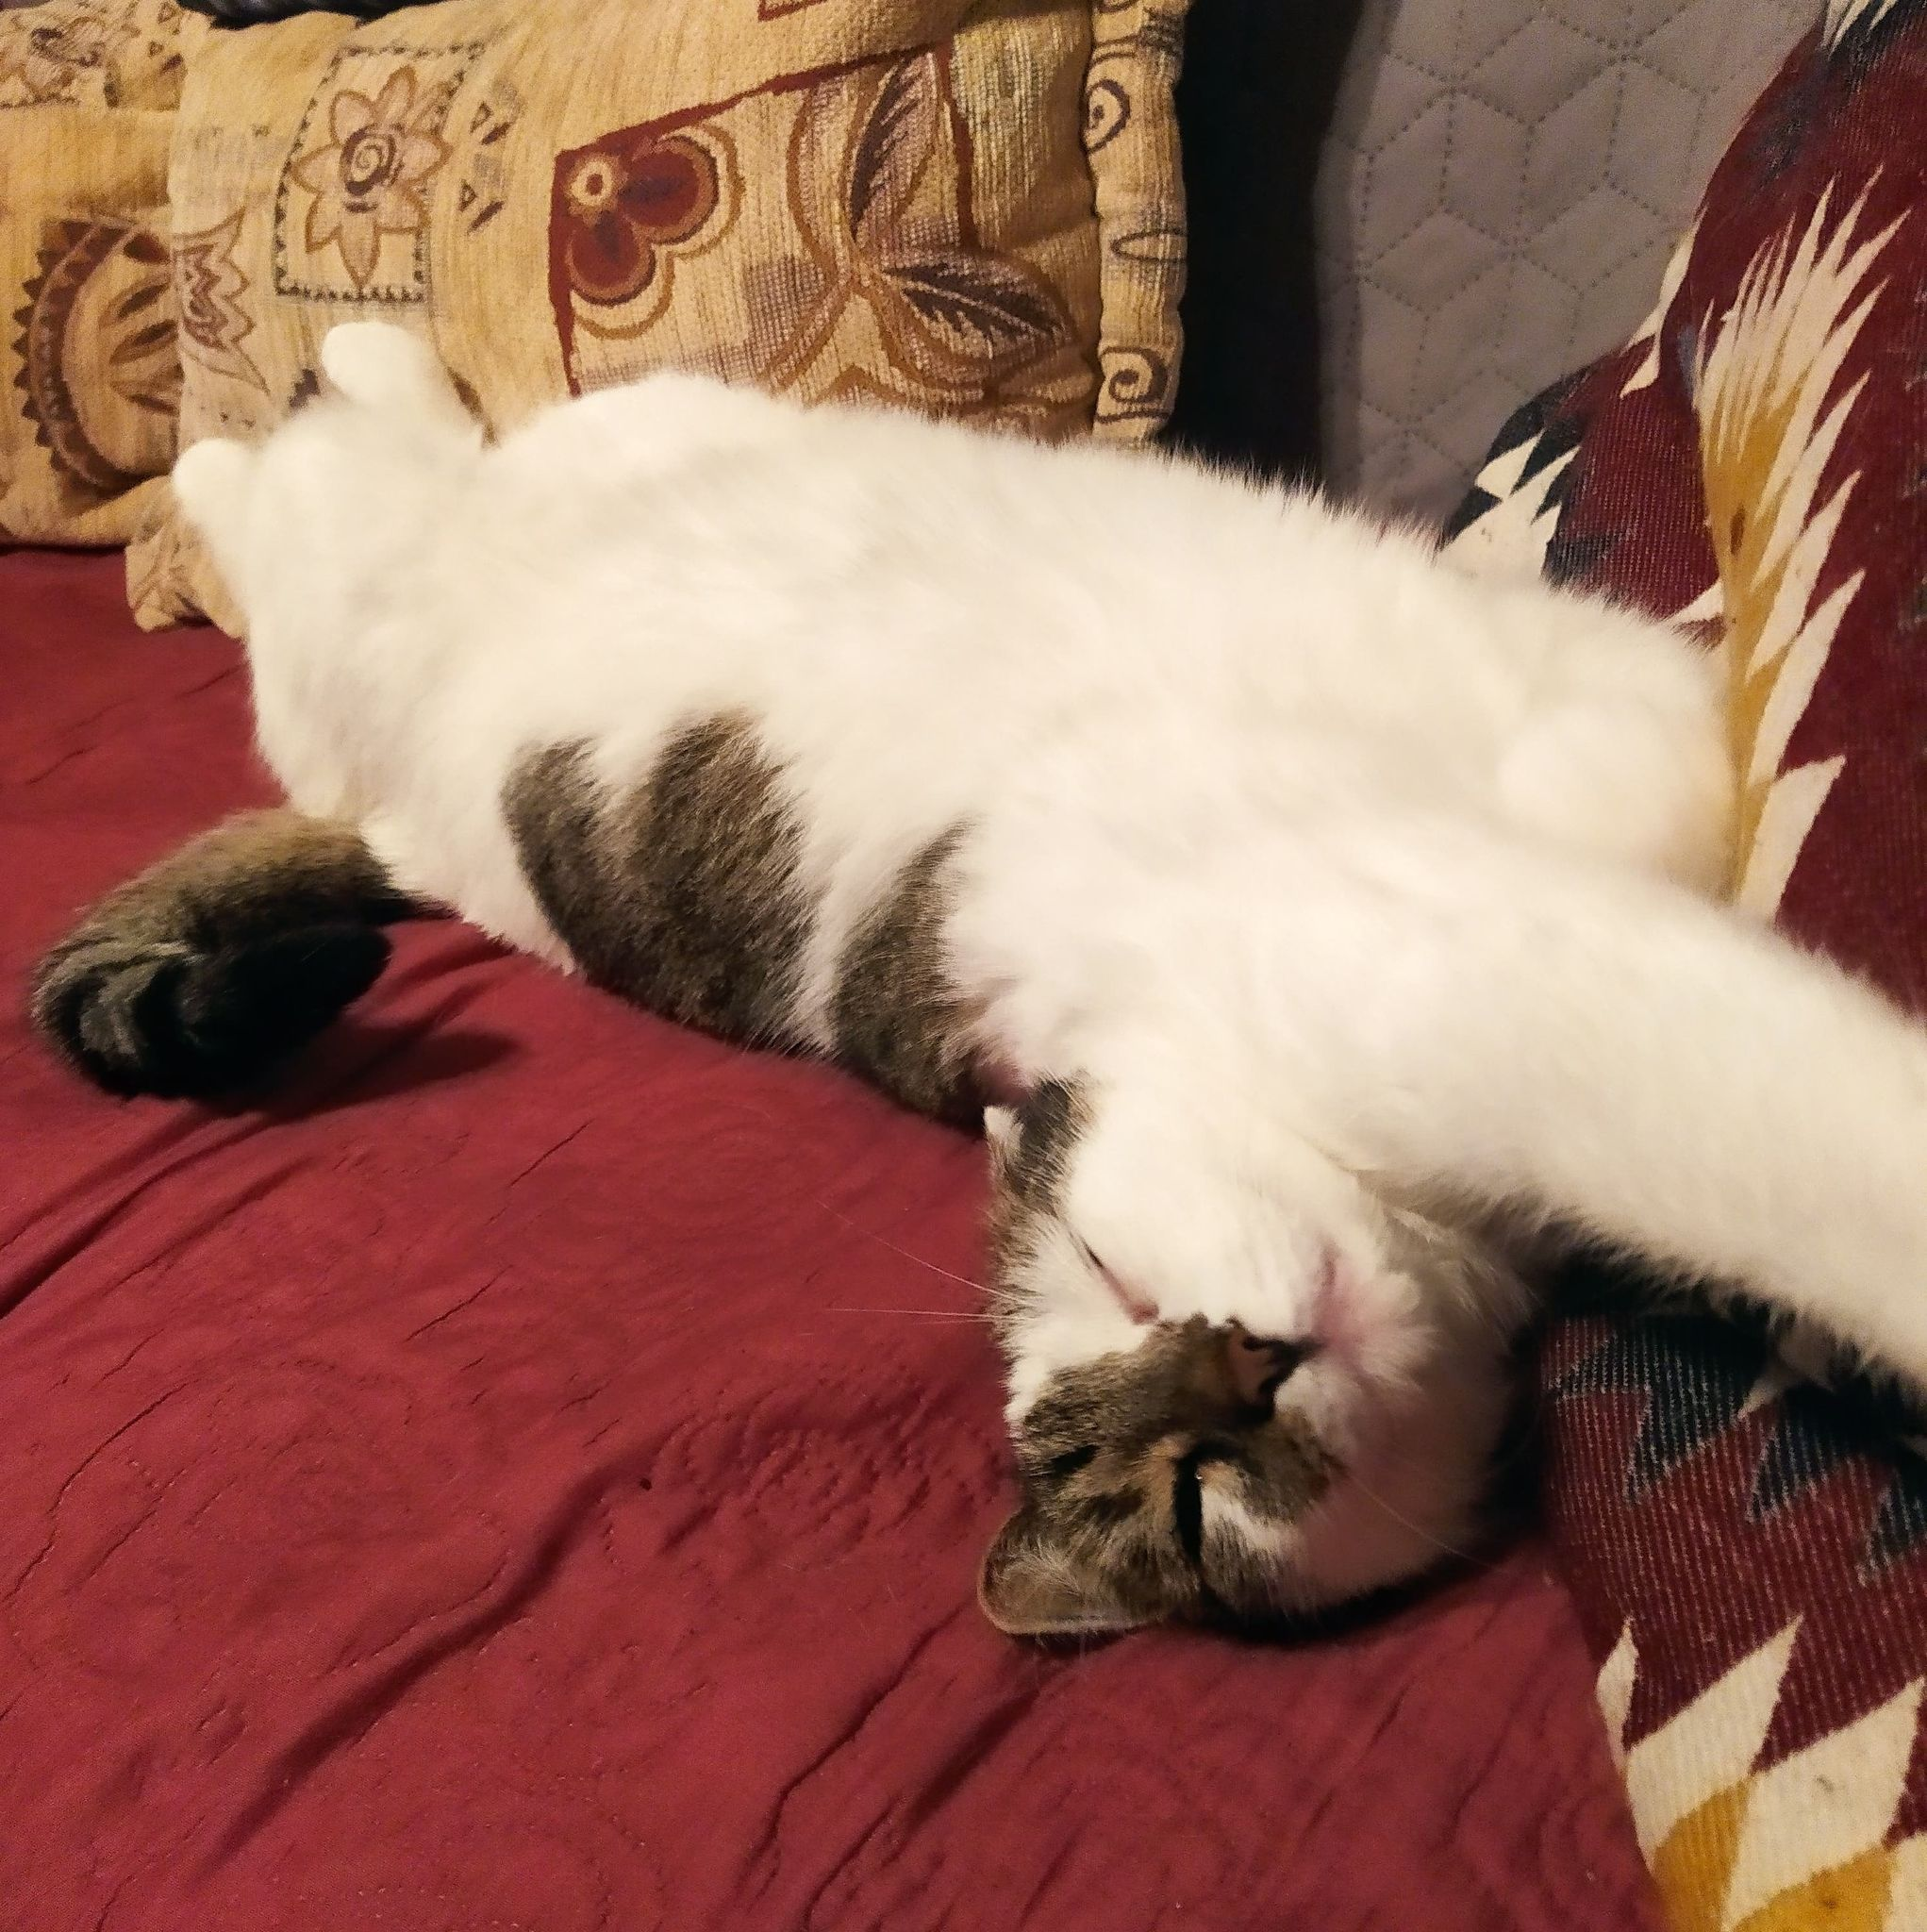
\includegraphics[width=0.6\textwidth]{./kytel.jpg}

{\slshape\scriptsize as long as algebra is taught in school, there will be prayer in school}
\end{center}

\newpage
\pagestyle{fancy}
\fancyhead{} % clear all header fields
\fancyhead[R]{\textbf{Algebra 2R}}
\fancyfoot{} % clear all footer fields
\fancyfoot[C]{\thepage}
\fancyfoot[L]{\color{black!20}Weronika Jakimowicz}
\fancyfoot[R]{\color{black!20}Według wykładu Prof. Newelskiego}

%Czwartek 23.03 godz. 18-20 -- odrabianie wykładu

%Pomoce dydaktyczne:
%\href{https://www.youtube.com/playlist?list=PL8yHsr3EFj53Zxu3iRGMYL_89GDMvdkgt}{playlista z losowymi wykladami}

% \subsection*{SYLABUS:}

% \deff{I. Podstawy teorii równań algebraicznych}

% \indent 1. Rozszerzenia ciał. Rozszerzenia o pierwiastek wielomianu nierozkładalnego. Ciało rozkładu wielomianu: istnieje, jedyność.

% \indent 2. Ciało algebraicznie domknięte: definicja. Każde ciało zawiera się w ciele algebraicznie domkniętym (konstrukcja). Podciało proste: istnienie, jedyność. Ciała proste.

% \indent 3. Pierwiastki z jedności, pierwiastki pierwotne. Grupa pierwiastków z jedności w ciele: każda jej skończona podgrupa jest cykliczna. Wielomiany podziału koła. Funkcja Frobeniusa. Ciała skończone: własności.
% \smallskip

% \deff{II. Teoria Galois}

% \indent 1. Rozszerzenia [elementy] algebraiczne, przestępne: definicja. Stopień rozszerzenia. Warunki równoważne algebraiczności. Wielomian minimalny elementu ciała nad podciałem, własności.

% \indent 2. Algebraiczne domknięcie ciała: definicja, istnienie, jedyność, własności (jednorodność). Istnienie rzeczywistych liczb przestępnych, liczby Liouville'a.

% \indent 3. Rozszerzenia normalne: definicja, własności. Rozszerzenia [elementy, wielomiany] rozdzielcze. Twierdzenie Abela o elemencie pierwotnym. Rozszerzenia czysto nierozdzielcze (radykalne): definicja, własności. Stopień rozdzielczy [radykalny] rozszerzenia: definicja, własności.

%\newpage 

\tableofcontents

\newpage

\newpage

\section{Wykład 1: Teoria równań algebraicznych}

Przez $R, S$ będziemy oznaczać pierścienie przemienne z $1\neq0$, natomiast $K, L$ będziemy rezerwować dla oznaczeń ciał.

\subsection{Rozwiązywanie układów równań}

Rozważmy funkcje $f_1,...,f_m\in R[X_1, ..., X_n]$. Dla wygody będziemy oznaczać krotki przez $\overline X$, czyli $R[X_1,...,X_n]=R[\overline X]$. Pojawia się problem: \dyg{czy istnieje rozszerzenie pierścieni z jednością $R\subseteq S$ takie, że układ $U:f_1(\overline X)=...=f_m(\overline X)=0$ ma rozwiązanie w pierścieniu $S$?}

\begin{fakt}
    $\overline a=(a_1,...,a_n)\subseteq S$, gdzie $S$ jest rozszerzeniem pierścienia $R$, jest \acc{rozwiązaniem układu równań} $U\iff g(\overline a)=0$ dla każdego wielomianu $\color{blue}g\in (f_1,...,f_m)\normalsubgroup R[X]$.
\end{fakt}

\textbf{Dowód:} 

$\impliedby$ Implikacja jest dość trywialna, jeśli każdy wielomian z $(f_1,...,f_m)$, czyli wytworzony za pomocą sumy i produktu wielomianów $f_1,...,f_m$ zeruje się na $\overline a$, to musi zerować się też na każdym z tych wielomianów.

$\implies$ Rozważamy dwa przypadki:

\indent 1. $(f_1,...,f_m)\ni b\neq 0$ i $b\in R$. 

To znaczy w $(f_1,...,f_m)$ mamy pewien niezerowy wyraz wolny. Wtedy mamy wielomian $g\in(f_1,...,f_m)$ taki, że $g(\overline a)\neq 0$. Ale przecież $g$ jest kombinacką wielomianów $f_1,...,f_m$, która na $\overline a$ przyjmują wartość $0$. W takim razie dostajemy układ sprzeczny i przypadek jest do odrzucenia.

\indent 2. $(f_1,...,f_m)\cap R=\{0\}$. (nie ma wyrazów wolnych różnych od $0$)

Teraz wiemy, że układ $U$ jest niesprzeczny, a więc możemy skonstruować pierścień z $1$ $S$ będący rozszerzeniem $R$ [$S\supseteq R$] oraz rozwiązanie $\overline a\subseteq S$ spełniające nasz układ równań.

Niech $S=R[\overline X]/(f_1,...,f_m)$ i rozważmy
$$j:R[\overline X]\to S=R[\overline{X}]/(f_1,...,f_m)$$
nazywane \acc{przekształceniem ilorazowym}. Po pierwsze, zauważmy, że $j\obciete R$ jest $1-1$, bo
$$\ker(j\obciete R)=\ker(j)\cap R=(f_1,...,f_m)\cap R=\{0\}$$
i dlatego
$$j\obciete R:R\izo{}j[R]\subseteq S.$$
Z uwagi na ten izomorfizm, będziemy utożsamiać $R, j[R]$. W takim razie, $S$ jest rozszerzeniem pierścienia $R$. Czyli mamy rozszerzenie pierścienia $R$.

Niech 
$$\overline a=(a_1,...,a_m)=(j(X_1),...,j(X_n))\subseteq S,$$
czyli jako potencjalne rozwiązanie rozważamy zbiór obrazów wielomianów stopnia $1$ przez wcześniej zdefiniowaną funkcję $j:R[\overline X]\to S$. Tak zdefiniowane $\overline a$ jest rozwiązaniem układu $U$ w pierścieniu $S$, bo dla funkcji wielomianowej (czyli zapisywalnej jako wielomian) $\hat{f_i}\in(f_1,...,f_m)$ mamy
$$\hat{f_i}(\overline a)=\hat{f_i}(j(X_1),...,j(X_m))=j(\hat{f_i}(X_1,...,X_m))=j(f_i)=0.$$

{\color{orange}\large TUTAJ TRZEBA POUZASADNIAĆ KILKA RÓWNOŚCI, ALE MOŻE NIE BĘDĘ TEGO ROBIŁA NA AISD}

\begin{uwaga}
    \label{uwaga1:1:2-warunek-rozwiazanie-ogolne}
    Skonstruowane powyżej {rozwiązanie $\overline a$} układu $U$ ma następującą własność {uniwersalności}:

    ($\coffee$) Jeżeli $S'\supseteq R$ jest rozszerzeniem pierścienia z $1$ i $\overline a'=(a_1',...,a_m')\subseteq S$ jest rozwiązaniem $U$ w $S'$, to istnieje jedyny homomorfizm 
    $$h:R[\overline a]\to R[\overline a']$$ 
    taki, że $h\obciete R$ jest identycznością na $R$ i $h(\overline a)=\overline a'$. \acc{Wszystkie rozwiązania układów są homomorficzne.}
\end{uwaga}

\begin{illustration}
    \node (R) at (0, 0) {$R$};
    \node (R[a]) at (4, 0) {$R[\overline a]\subseteq S$};
    \node (R[a']) at (0, -3) {$R[\overline a']\subseteq S'$};
    \draw [ ->] (R)--(R[a]) node [midway, above] {$\subseteq$};
    \draw [->] (R)--(R[a']) node [midway, left] {$\subseteq$};
    \draw[->] (R[a])--(R[a']) node [midway, right] {$h$};
\end{illustration}

Tutaj \deff{$R[\overline a]\subseteq S$ jest podpierścieniem generowanym przez $R\cup\{\overline a\}$}, czyli zbiór:
$$R[\overline a]=\{f(\overline a)\;:\;f(\overline X)\in R[\overline X]\}\subseteq S$$

\textbf{Dowód:} Niech $I=\{g\in R[\overline X]\;:\;g(\overline a')=0\}\subseteq S'$. Oczywiście mamy, że $I\normalsubgroup R[\overline X]$, a więc
$$(f_1,...,f_m)\subseteq I.$$
Z twierdzenia o faktoryzacji wie
\begin{illustration}
    \node (R[x]) at (0, 0) {$R[\overline X]$};
    \node (S) at (4, 0) {$S=R[\overline X]/(f_1,...,f_m)$};
    \node (R[a']) at (0, -3) {$S'\supseteq R[\overline a']$};
    \draw[->] (R[x])--(S) node [midway, above] {$j$};
    \draw[->] (R[x])--(R[a']) node [midway, left] {$\phi$};
    \draw[->, dashed] (S)--(R[a']) node [midway, right] {$(\exists\;!h)\;h(\overline a)=\overline a'$};
\end{illustration}
Homomorfizm $\phi:R[\overline X]\to R[\overline a']$ określamy wzorem
$$\phi(w)=w(\overline a),$$
a homomorfizm $j$ jest jak wyżej odwzorowaniem ilorazowym. Widzimy, że 
$$I=\ker(\phi)$$
$$\ker(j)=(f_1,...,f_m).$$
Z twierdzenia o homomorfizmie pierścieni dostajemy jedyny homomorfizm 
$$h:R[X]/(f_1,...,f_m)\to R[\overline a]$$
taki, że $h(\overline a)=\overline a'$.

\begin{uwaga}
    Jeśli $I=(f_1,...,f_m)$, to $h:R[\overline a]\izo R[\overline a']$.
\end{uwaga}

Wtedy mamy $\ker\phi=\ker j$, czyli $\ker(h\circ j)=\ker\phi=\ker j$, no a z tego wynika, że $\ker h$ jest trywialne, czyli $h$ jest apimorfizmem (1-1). Z drugiej strony, $Im \phi=Im(h\circ j)$, a $\phi$ jest epimorfizmem ("na"), więc również $h$ musi być "na".
\medskip

\begin{important}
Załóżmy, że $S\supseteq R$ jest rozszerzeniem pierścienia oraz $\overline a\in S^n$. Wtedy:

\indent 1. ideał $\overline a$ nad $R$ definiujemy jako 
$$\color{blue}I(\overline a/R)=\{g\in R[\overline X]\;:\;g(\overline a)=0\}$$

\indent 2. $\overline a$ nazywamy \deff{rozwiązaniem ogólnym} układu $U$, jeśli ideał 
$$I(\overline a/R)=(f_1,...,f_m).$$
\end{important}

\begin{uwaga}
    W sytuacji jak z definicji wyżej, gdy $U$ jest układem niesprzecznym, wtedy 
    
    $\overline a$ jest rozwiązaniem ogólnym układu $U$ $\iff$ zachodzi warunek \hyperref[uwaga1:1:2-warunek-rozwiazanie-ogolne]{(\coffee)}.
\end{uwaga}

\textbf{Dowód:} Ćwiczenia.

\subsection{Rozszerzanie ciał}

Dla $K\subseteq L$ ciał i $\overline a\subseteq L$ definiujemy \deff{ideał $\overline a$ nad $K$} jako:
$$\color{blue}I(\overline a /L):=\{f(X_1,...,X_n)\in K[\overline X]:f(\overline a)=0\},$$
to znaczy generujemy ideał w wielomianach nad $K$ zawierający wszystkie wielomiany (niekoniecznie tylko jednej zmiennej) zerujące się w $\overline a$. 
\medskip

\textbf{Przykład:}
\smallskip

Dla $K=\Q,L=\R,n=1,a_1=\sqrt{2}$ mamy
$$I(\sqrt{2}/\Q)=\{f(x^2-2)\;:\;f\in\Q[X]\}=(x^2-2)\normalsubgroup \Q[X]$$

Dalej, definiujemy
$$\color{blue}K[\overline a]:=\{f(\overline a)\;:\;f\in K[X]\}$$
czyli \deff{podpierścień $L$ generowany przez $K\cup\{\overline a\}$} oraz \deff{$K(\overline a)$, czyli podciało $L$} generowane przez $K\cup\{\overline a\}$:
$$\color{blue}K(\overline a):=\{f(\overline a)\;:\;f\in K(X_1,...,X_n)\;i\;f(\overline a)\text{ dobrze określone}\}.$$
Tutaj $K(X_1,...,X_n)$ to \dyg{ciało ułamków pierścienia} $K[\overline a]$ w ciele $L$ (czyli najmniejsze ciało, że pierścień może być w nim zanurzony). Czasami oznaczamy to przez $K[\overline a]_0$.
\medskip

% \textbf{Przykład:}
% \smallskip

% Dla $K=\Q,L=\R$ zachodzi:
% $$K[\sqrt2]=\Q[\sqrt2]=\{q+p\sqrt2\;:\;q,p\in\Q\}$$
% $$K[\sqrt2,\sqrt3]=\Q[\sqrt2,\sqrt3]$$
% $$K(\sqrt2)=\Q[\sqrt2]$$
% to ostatnie to usuwanie niewymierności z mianownika.
% \medskip

\begin{uwaga}
    \label{uwga:1:1:5}
    Niech $K\subseteq L_1,K\subseteq L_2$ będą ciałami. Wybieramy $\overline a_1\in L_1$ i $\overline a_2\in L_2$, $|\overline a_1|=|\overline a_2|=n$. Wtedy następujące warunki są równoważne:

\indent 1. istnieje izomorfizm $\phi:K[\overline a_1]\to K[\overline a_2]$ taki, że $\phi\obciete K=id_K$ oraz $\phi(\overline a_1)=\overline a_2$.

\indent 2. $I(\overline a_1/K)=I(\overline a_2/K)$.
\end{uwaga}

\textbf{Dowód:}

%\begin{center}
% $K[\overline a]\isomorphism K[\overline b]$ \acc{$\implies$} $I(\overline a/K)=I(\overline b/K)$

% Niech $\omega\in K[\overline X]$. Wtedy $\omega\in I(\overline a/K)$ wtedy i tylko wtedy, gdy $\omega(\overline a)=0$, to mamy z definicji $I(\overline a/K)$. Wiemy też, że $\phi(a)\in K[\overline X]$ wtedy, gdy $\omega(\phi(\overline a))=0$, a ponieważ $\phi(\overline a)=\overline b$, to również $\omega(\overline b)=0$ i mamy, że $\omega\in I(\overline b/K)$. Czyli izomorfizm między $K[\overline a]=K[\overline b]$ implikuje, że $I(\overline a/K)=I(\overline b/K)$.
% \smallskip

% $K[\overline a]\isomorphism K[\overline b]$ \acc{$\impliedby$} $I(\overline a/K)=I(\overline b/K)$

% Spróbujmy zdefiniować izomorfizm $\phi$ tak, że dla $\omega\in K[\overline X]$ mamy $\phi(\omega(\overline a))=\omega(\overline b)$

% 1. $\phi$ jest homomorfizmem: 
% $$\phi(\omega(\overline a)\cdot v(\overline a))=f((\omega\cdot v)(\overline a))=(\omega\cdot v)(\overline b)=\omega(\overline b)\cdot v(\overline b)=\phi(\omega(\overline a))\cdot \phi(v(\overline a))$$

% 2. $\phi$ jest różnowartościowe:
% $$\phi(\omega(\overline a))=\phi(v(\overline a))\iff \omega(\overline b)=v(\overline b)\iff (\omega-v)(\overline b)=0\iff \omega-v\in I(\overline b/K)=I(\overline a/K)\iff (\omega-v)(\overline a)=0\iff \omega(\overline a)=v(\overline a)$$

% 3. $\phi$ jest dobrze zdefiniowane (czyli przyjmuje tylko jedną wartość dla jednego argumentu):
% $$\omega(\overline a)-v(\overline a)=0\iff (\omega-v)(\overline a)=0\iff \omega -v\in I(\overline a/K)\iff \omega-v\in I(\overline b/K)\iff (\omega-v)(\overline b)=0\iff \omega(\overline b)-v(\overline b)=0$$

% \podz{dark-green}
% \bigskip

% Możemy teraz zapytać, czy każdy ideał w pierścieniu wielomianów $K[X]$ jest postaci $I(\overline a/K)$ dla pewnego $\overline a\in L\supset K$? Albo ogólniej, czy dla pierścienia przemiennego $R$ z $1_R\neq0_R$ oraz ideału $I=(f_1,...,f_m)=I(\overline a/R)\normalsubgroup R[X]$, czy istnieje nadpierścień $S$ taki, że $1_S=1_R$ i $0_S=0_R$ oraz układ
% $$f_1(\overline x)=...=f_m(\overline m)=0$$
% ma rozwiązanie w $S$? Takie rozwiązanie spełniałoby $\overline a\in S\iff (\forall\;g\in(f_1,...,f_m))\;g(\overline a)=0$.
%\end{center}

$1\implies 2$

Implikacja jest jasna, bo dla $g(\overline X)\in K[\overline X]$, bo $g(\overline a_1)=0$ w $K[\overline a_1]$ $\iff$ $g(f(\overline a_1))=0$, a $f(\overline a_1)=\overline a_2$.

$1\impliedby 2$

Zwróćmy uwagę na odwzorowanie ewaluacji $\overline a_1$
$$\phi_{\overline a_1}:K[\overline X]\xrightarrow[]{"na"}K[a_1]$$
zadane wzorem
$$\phi(w(\overline X))=w(\overline a_1).$$
Mamy
$$\ker(\phi_{\overline a_1})=I(\overline a_1/K).$$

Tak samo dla $\overline a_2$ możemy określić analogicznie odwzorowanie ewaluacyjne $\phi_{\overline a_2}:K[\overline X]\to K[\overline a_2]$. Wtedy
$$I(\overline a_2/K)=\ker(\phi_{\overline a_2}),$$
ale ponieważ $I(\overline a_1/K)=I(\overline a_2/K)$, to $\ker(\phi_{\overline a_1})=\ker(\phi_{\overline a_2})$. Oznaczmy $I=I(\overline a_1/K)=I(\overline a_2/K)$. Widzimy, że $\phi_{\overline a_i}\obciete K=id_k$.

\begin{illustration}
    \node (K) at (4, 0) {$K[\overline X]$};
    \node (K[a1]) at (0, -2) {$K[\overline a_1]$};
    \node (K[a2]) at (8, -2) {$K[\overline a_2]$};
    \node (K[X]/I) at (4, -2.5) {$K[X]/I$};
    \draw[->] (K)--(K[a1]) node [midway, left] {$\phi_{\overline a_1}$};
    \draw[->] (K)--(K[a2]) node [midway, right] {$\phi_{\overline a_2}$};
    \draw[->] (K)--(K[X]/I) node [midway, right] {$j${\scriptsize - ilorazowe}};
    \draw[->, dashed] (K[X]/I)--(K[a1]) node [midway, below] {$f_1$} node [midway, above] {$\cong$};
    \draw[->, dashed] (K[X]/I)--(K[a2]) node [midway, below] {$f_2$} node [midway, above] {$\cong$};
\end{illustration}

Niech $f=f_2f_1^{-1}:K[\overline a_1]\to K[\overline a_2]$ jest funkcją spełniającą warunki punktu 1.

{\large\color{orange}MOŻE TUTAJ ŁADNIE SPRAWDZIĆ ŻE NAPRAWDĘ JEST TO DOBRZE SPEŁNIAJĄCA WARUNKI FUNKCJA?}

\textbf{\large\color{yellow}Uwaga.}
    \emph{Niech $I\normalsubgroup K[\overline X]$ \acc{noetherowskiego} pierścienia $K[\overline X]$. Niech $I=(f_1,...,f_m)$ dla pewnych $f_i\in K[\overline X]$. Wtedy istnieje rozszerzenie pierścienia $S\supseteq K$ oraz $\overline a\subseteq S$ - rozwiązanie ogólne układu $f_1(\overline X)=...=f_m(\overline X)=0$ takie, że $\color{blue}I(\overline a/K)=I$.}

\textbf{Dowód:} Wcześniejsze uwagi {\large\color{orange}KTÓRE KONKRETNIE?}

\begin{tw}
    Niech $I\normalsubgroup K[\overline X]$. Wtedy istnieje ciało $L\supseteq K$ oraz $\overline a=(a_1,...,a_n)\subseteq L$ takie, że $f(\overline a)=0$ dla każdego $f\in I$.
\end{tw}

\textbf{Dowód:} Niech $I\subseteq M\normalsubgroup K[\overline X]$ będzie ideałem maksymalnym. Niech $L=K[\overline X]/M$ i określmy przekształcenie ilorazowe
$$j:K[\overline X]/M\to L=K[\overline X]/M.$$
Ponieważ $M\cap K=\{0\}$ (bo inaczej w ideale byłby wielomian odwracalny), to $j\obciete K:K\to L$ jest funkcją $1-1$, czyli
$$j\obciete K:K\xrightarrow[]{1-1}j[K]\subseteq L.$$
Możemy utożsamić $K$ z $j[K]$, czyli $K\subseteq L$. Niech $\overline a=(a_1,..., a_n)$ takie, że dla każdego $i\in[n]$ 
$$a_i=j(X_i)\in L.$$
Wtedy $g(\overline a)=0$ dla każdego $g(\overline X)\in M\supseteq I$ (bo inaczej mielibyśmy wyrazy wolne).

\begin{wniosek}
    \label{wniosek1:2:4}
    Niech $f\in K[X]$ stopnia $>0$. Wtedy istnieje ciało $L\supseteq K$ rozszerzające ciało $K$ takie, że $f$ ma pierwiastek w ciele $L$.
\end{wniosek}

\textbf{Przykłady:}

\indent 1. Rozpatrzmy ciało $K=\Q$ i $f(X)=X-2$. Wtedy $I=(f)\normalsubgroup\Q[X]$ jest ideałem maksymalnym, bo jest on pierwszy (w tym wypadku nierozkładalny). Równanie $f=0$ ma rozwiązanie ogólne w pierścieniu ilorazowym
$$\Q[X]/I\cong \Q.$$
Czyli nie zawsze musimy rozszerzać ciało do czegoś nowego.

\indent 2. $\C=\R[i]=\R(i)=\R[z]$ dla każdego $z\in\C\setminus\R$, co jest na liście zadań.
\medskip

Załóżmy, że $K\subseteq L_1, K\subseteq L_2$ są rozszerzeniami ciała. Wtedy mówimy, że \deff{$L_1$ jest izomorficzne z $L_2$ nad $K$} [\acc{$L_1\cong_KL_2$}] $\iff$ istnieje izomorfizm $f:L_1\to L_2$ taki, że $f\obciete K=id_K$.

\begin{fakt}{\color{back}dupa }
\label{fakt:1:2:5}

\indent 1. Załóżmy, że $f(X)\in K[X]$ jest nierozkładalny. Niech $L_1=K(a_1)$, $L_2=K(a_2)$ i $f(a_i)=0$ w $L_i$. Wtedy $L_1\cong_KL_2$.

\indent 2. Ogółniej: załóżmy, że $\phi:K_1\to K_2$ jest izomorfizmem i $f_1\in K_1[X],f_2\in K_2[X]$, $\phi(f_1)=f_2$, $f_i$ jest nierozkładalne. Dodatkowo załóżmy, że $L_1=K_1(a_1)$ i $L_2=K_2(a_2)$, gdzie $f_i(a_i)=0$ w $L_i$. Wtedy istnieje \acc{izomorfizm $\phi\in\psi:L_1\to L_2$ taki, że $\psi(a_1)=a_2$.}
\end{fakt}

\textbf{Dowód:}

\indent 1. $I(a_1/K)=(f)=I(a_2/K)$, stąd na mocy \ref{uwga:1:1:5} mamy $K(a_1)\cong_KK(a_2)$. Po dowodzie przypadku 2. możemy uzasadniać, że jest to szczególny przypadek tego ogólniejszego stwierdzenia właśnie.

\indent 2. Zacznijmy od rozrysowania tej sytuacji:

\begin{illustration}
    \draw (-2, 0) ellipse (1.5 and 0.7) node [below] {$K_1$};
    \draw (2, 0) ellipse (1.5 and 0.7) node [below] {$K_2$};
    \draw (-3.5, 0)..controls (-3, 3) and (-1, 3)..(-0.5, 0) node [midway, above] {$L_1$};
    \draw (3.5, 0)..controls (3, 3) and (1, 3)..(0.5, 0) node [midway, above] {$L_2$};
    \draw[->] (-2, 1)..controls (-1, 2) and (1, 2)..(2, 1) node [midway, below] {$\psi$} node [midway, above] {$\cong$};
    \draw[->] (-1.2, -0.6)..controls (-0.8, -1) and (0.8, -1)..(1.2, -0.6) node [midway, below] {$\phi$} node [midway, above] {$\cong$};
\end{illustration}

Izomorfizm $\phi:K_1[X]\izo K_2[X]$ indukuje nam przekształcenie
$$K_1[X]/(f_1)\izo{\phi} K_2[X]/(f_2),$$
bo $\phi(f_1)=f_2$. Wiemy, że $f_i$ jest nierozkładalne, czyli
$$I(a_i/K_i)=(f_i)\normalsubgroup K_i[X]$$
jest ideałem maksymalnym. Mamy
$$L_i=K_i(a_i)=K_i[a_i]\cong K[X]/I(a_i/K_i).$$

\begin{illustration}
    \node (K1) at (0, 0) {$K_1[X]$};
    \node (K2) at (4, 0) {$K_2[X]$};
    \draw[->] (K1)--(K2) node [midway, above] {$\cong$} node [midway, below] {$\phi$};
    \node (K1f) at (0, -2) {$K_1[X]/(f_1)$};
    \node (K2f) at (4, -2) {$K_2[X]/(f_2)$};
    \draw[->] (K1f)--(K2f) node [midway, below] {$\phi$} node [midway, above] {$\cong$};
    \draw[->] (2, -.7)--(2, -1.3);
    \node (L1) at (0, -4) {$L_1=K_1(a_1)$};
    \node (L2) at (4, -4) {$L_2=K_2(a_2)$};
    \draw[->] (L1)--(L2) node [midway, above] {$\cong$} node [midway, below] {$\psi$};
    \node (K1) at (0, -5) {$K_1$};
    \node (K2) at (4, -5) {$K_2$};
    \draw[->] (K1)--(K2) node [midway, below] {$\phi$};
    \node[rotate=90] at (0, -4.5) {$\subseteq$};
    \node[rotate=90] at (4, -4.5) {$\subseteq$};
    \draw[->] (K1f)--(L1) node [midway, left] {$\cong$} node [midway, right] {$h_1$};
    \draw[->] (K2f)--(L2) node [midway, left] {$\cong$} node [midway, right] {$h_2$};
\end{illustration}

\newpage
 
\section{Wykład 2: Ciała skończone i pierwiastki z jedności}

\begin{important}
Ciało $L\supseteq K$ nazywamy \deff{ciałem rozkładu nad $K$} wielomianu $f\in K[X]$, gdy spełnione są warunki:

\indent 1. $f$ rozkłada się w pierścieniu $L[X]$ na czynniki liniowe (stopnia $1$)

\indent 2. Ciało $L$ jest rozszerzeniem ciała $K$ o elementy $a_1,...,a_n$, gdzie $a_1,...,a_n$ to wszystkie pierwiastki $f$ w $L$.
\end{important}

\textbf{Przykład:} Jeżeli $deg(f)=0$, to nie istnieje ciało rozkładu $f$.

\begin{wniosek}
    Załóżmy, że $f\in K[X]$ jest wielomianem stopnia $>0$. Wtedy

\indent 1. istnieje $L$: ciało rozkładu $f$ nad $K$,

\indent 2. to ciało jest jedyne z dokładnością do izomorfizmy nad $K$.
\end{wniosek}

\textbf{Dowód:}

\indent 1. Dowód przez indukcje względem stopnia $f$

Jako przypadek bazowy rozważmy $f$ takie, że $deg(f)=1$. Wtedy $L=K$ i wszystko wniosek jest spełniony.

Załóżmy teraz, że stopień wielomianu $f$ jest $>1$ i tez zachodzi dla wszystkich wielomianów stopnia $<deg(f)$ i wszystkich ciał $K'$. Teraz z \ref{wniosek1:2:4} wiemy, że istnieje rozszerzenie ciała $L\supseteq K$ takie, że $f$ ma pierwiastek w $L$. Nazwijmy ten pierwiastek $a_0$ i niech
$$K'=K(a_0).$$
Ponieważ $K'[X]$ wielomian $f$ ma pierwiastek $a_0$, to możemy zapisać
$$f=(x-a_0)f_1$$
dla pewnego $f_1\in K'[X]$ i $deg(f_1)<deg(f)$. Z założenia indukcyjnego dla $f_a$ istnieje $L'=K'(a_1,...,a_r)$ - ciało rozkładu wielomianu $f_1$ nad $K'$. Wtedy 
$$L=K(a_0,...,a_r)$$
jest ciałem rozkładu $f$ nad $K$.

\indent 2. Udowodnimy wersję ogólniejszą: 
\phantomsection
\label{stwierdzenie:wniosek}

\emph{(\bat) Jeśli $\phi:K_1\izo{} K_2$ jest izomorfizmem nad ciałem i $f_i\in K_i[X]$ jest wielomianem stopnia $>0$, $\phi(f_1)=f_2$, to wtedy istnieje $ \psi:L_1\izo{} L_2$ izomorfizm nad ciałami rozkładu $f_i$ w $K_i$ rozszerzający izomorfizm $\phi$ (to znaczy $\phi\subseteq \psi$).}

Wykorzystamy indukcję po $deg(f)$. W przypadku bazowym mamy $deg(f)=1$, czyli $L_1=K_1,L_2=K_2$ i $\phi=\psi$.

Teraz niech $deg(f)>1$ i załóżmy, że dla wszystkich ciał $K'$ oraz wielomianów stopnia $<deg(f)$ jest to prawdą. Niech
$$f_i=f_i'\cdot g_i,$$
gdzie $f_i',g_i\in K_i[X]$ i $g_i$ jest wielomianem nierozkładalnym w $K$. Wiemy już, że istnieje $a_i\in L_i$ będące pierwiastkiem wielomianu $g_i$.

Z faktu \ref{fakt:1:2:5}:(2), wiemy, że istnieje wtedy izomorfizm
$$\psi_0:K_1(a_1)\izo{}K_2(a_2)$$
taki, że $\psi_0(a_1)=a_2$ i $\phi\subseteq\psi_0$.

\begin{illustration}
    \node (K1) at (0, 0) {$K_1(a_1)$};
    \node (K2) at (4, 0) {$K_2(a_2)$};
    \node (L1) at (0, -2.3) {$L_1$};
    \node (L2) at (4, -2.3) {$L_2$};
    \draw[->] (K1)--(K2) node [midway, above] {$\cong$} node [midway, below] {$\exists\;\psi_0$};
    \draw[->] (L1)--(L2) node [midway, above] {$\cong$} node [midway, below] {$\exists\;\psi_1$};
    \node [rotate=90] (=1) at (0, -0.5) {$=$};
    \node [rotate=90] (=1) at (4, -0.5) {$=$};
    \node (K1') at (0, -1) {$K_1'$};
    \node (K2') at (4, -1) {$K_2'$};
    \node [rotate=90] at (0, -1.65) {$\supseteq$};
    \node [rotate=90] at (4, -1.65) {$\supseteq$};
\end{illustration}

Mamy, że {\large\color{orange}$L_i$ to ciało rozkładu $f_i'$ nad $K_i$}. W takim razie z założenia indukcyjnego istnieje izomorfizm
$$\psi_1:L_1\izo{}L_2$$
taki, że $\psi\subseteq\psi_0$ i to już jest koniec.

\begin{wniosek}
    Jeśli $f_1\in K_1[X]$ i $f_2\in K_2[X]$ są nierozkładalnymi wielomianami, $\phi:K_1\izo{}K_2$ izomorfizmem i $\phi(f_1)=f_2$, a $L_1,L_2$ to ciała rozkładu $f_1,f_2$ odpowiednio nad $K_1$ i $K_2$, $a_i\in L_i$ to pierwiastek $f_i$, to wtedy istnieje $\psi:L_1\izo{}L_2$ takie, że $\psi(a_1)=a_2$.
\end{wniosek}

\textbf{Dowód:} Wynika z dowodu stwierdzenia \hyperref[stwierdzenie:wniosek]{\bat}.

\subsection{Algebraiczne domknięcie ciała}

Ciało $L$ jest \deff{algebraicznie domknięte} $\iff$ dla każdego $f\in L[X]$ o stopniu $>0$ istnieje pierwiastek $f$ w $L$, to znaczy każdy wielomian rozkłada się na czynniki liniowe nad $L$.

\textbf{Przykład:}

\indent \point $\C$ jest algebraicznie domknięte.

\indent \point $\R$ nie jest algebraicznie domknięte, gdyż $x^2+1$ nie ma pierwiastka rzeczywistego.

\indent \point $\Q[i]$ nie jest algebraicznie domknięte, bo $x^2-2$ nie ma pierwiastka.

\begin{tw}
    Każde ciało zawiera się w pewnym ciele algebraicznie domkniętym.
\end{tw}

\textbf{Dowód:}

\acc{Lemat:} Dla każdego ciała $K$ istnieje $K'\supseteq K$ takie, że $(\forall\;f\in K[X])$ stopnia $>0$ $f$ ma pierwiastek w $K'$.

Rozważmy dobry porządek na zbiorze wielomianów z $K[X]$ stopnia $>0$
$$\{f\in K[X]\;:\;deg(f)>0\}=\{f_\alpha\;:\;\alpha\subset x\}$$
Skonstruujmy rosnący ciąg ciał $\{K_\alpha\;:\;\alpha\subset x\}$ taki, że 

\indent \point $K\subseteq K_\alpha\subseteq K_\beta$ dla $\alpha<\beta< x$

\indent \point $f_\alpha$ ma pierwiastek w $K_{\alpha+1}$.

Załóżmy, że $\alpha<x$ i mamy $\{K_\beta\;:\;\beta<\alpha\}$.

\indent 1. $\alpha$ to liczba graniczna, wtedy $K_\alpha=\ubigcup\limits_{\beta<\alpha}K_\beta$

\indent 2. $\alpha=\beta+1$ to następnik, wtedy $K_\alpha=K_\beta(a)$, gdzie $a$ to pierwiastek wielomianu $f_\beta$.

Czyli lemat jest prawdziwy.

Wracamy teraz do dowodu twierdzenia i niech $(L_n,n<\omega)$ będzie rosnącym ciągiem ciał takim, że

\indent \point $L_0=K$

\indent \point $L_{n+1}\supseteq L_n$, gdzie $L_{n+1}$ dane jest przez lemat, to znaczy $(\forall\;f\in L_n[X])$ $f$ ma pierwiastek $L_{n+1}$.

Niech
$$\hat{K}=L_\infty=\ubigcup\limits_{n<\omega}L_n.$$
Jest to ciało, ponieważ suma rosnącego ciągu ciał jest ciałem. Dalej mamy, że również
$$L[X]=\ubigcup\limits_{n<\omega}L_n[X]$$
i $L[X]$ jest algebraicznie domknięte.

\begin{uwaga}
    Załóżmy, że mamy ciała $K\subseteq L$. Wtedy

\indent \point $char(K)=char(L)$

\indent \point $0_K=0_L$ oraz $1_K=1_L$

\indent \point $K^*=K\setminus\{0\}<L^*=L\setminus\{0\}$
\end{uwaga}

\subsection{Pierwiastki z jedności}

$K$ jest \deff{ciałem prostym} wtedy i tylko wtedy, gdy $K$ nie zawierza żadnego właściwego podciała. 

\textbf{Przykład:}

\indent \point $\Q$, gdzie $char(\Q)=0$ to ciało proste nieskończone.

\indent \point Ciałem prostym skończonym jest na przykład $\Z_p$ dla liczby pierwszej $p$, wtedy $char(\Z_p)=p$.
\medskip

Niech $R$ będzie pierścieniem przemiennym z $1\neq0$. Mamy następujące definicje:

\indent 1. $a\in R$ jest \deff{pierwiastkiem z $1$ }stopnia $n>0$ $\iff$ $a^n=1$

\indent 2. $\mu_n(R)=\{a\in R\;:\;a^n=1\}$ jest \deff{grupą pierwiastków z $1$} stopnia $n$

\indent 3. $\mu(R)=\bigcup\limits_{n>0}\mu_n(R)$ jest \deff{grupą pierwiastków z $1$}

\indent 4. $a$ jest \deff{pierwiastkiem pierwotnym} stopnia $n$ z $1$ $\iff$ $a\in\mu_n(R)$ oraz $(\forall\;k<n)a\notin\mu_k(R)$.

\begin{uwaga}{\color{back}dupa}

\indent 1. $\mu_n(R)\normalsubgroup R^X$ jest grupą jednostek pierścienia

\indent 2.$\mu(R)\normalsubgroup R^X$

\indent 3. $\mu(R)$ jest \acc{torsyjną grupą abelową} (każdy element jest pierwiastkiem z $1$).
\end{uwaga}

\textbf{Przykłady}

\indent 1. $\mu(\C)=\bigcup\limits_{n>0}\mu_n(\C)\lneq(\{z\in\C\;:\;|z|=1\},\cdot\})<\C^x=C\setminus\{0\}$

\indent 2. $\mu(\C)\cong(\Q,+)/(\Z,+)$, bo $f:\Q\xrightarrow[homo]{"na"}\mu(\C)$ taki, że $f(w)=\cos(w2\pi)+i\sin(w2\pi)$ ma jądro $ker(f)=\Z$.

\indent 3. $\mu(\R)=\{\pm1\}$

\indent 4. $\mu_n(K)=\{\text{zera wielomianu }w_n(x)=x^n-1\}$

\begin{uwaga}{\color{back}dupa}
    \label{uwaga:2:6}

\indent 1. Jeśli $char(K)=0$, to $w_n(x)=x^n-1$ ma tylko pierwiastki jednokrotne w $K$

\indent 2. Jeśli $char(K)=p>0$ i $n=p^ln_1$ takie, że $p\nmid n_1$, to wszystkie pierwiastki $w_n(x)=x^n-1$ mają krotność $p^l$ w $K$.
\end{uwaga}

\textbf{Dowód:}

\indent 1. Niech $a\in K$ takie, że $w_n(a)=0$. Z twierdzenia Bezouta mamy, że
$$w_n(x)=x^n-1=x^n-a^n=(x-a)(x^{n-1}+ax^{n-2}+...+a^{n-2}x+a^{n-1})=(x-a)v_n(x),$$
gdzie $v_n(x)=x^{n-1}+ax^{n-2}+...+a^{n-2}x+a^{n-1}$.

Z tego, że $char(K)=0$ wynika, że $v_n(a)=na^{n-1}+0$, skąd wynika, że $a$ jest jednokrotnym pierwiastkiem $w_n(x)$.

\begin{fakt}
    Załóżmy, że $char(K)=p>0$. Wtedy funkcja $f:K\to K$ taka, że $f(x)=x^p$ jest homomorfizmem ciał oraz monomorfizmem zwanym \deff{funkcją Frobeniusa}.
\end{fakt}

\begin{uwaga}
    $x\mapsto x^p$ nie musi być funkcją "na" (automorfizmem). Na przykład $K=\Z_p(f)$, wtedy $x\mapsto x^p$ nie jest "na".
\end{uwaga}

\indent 2. Mając powyższy fakt i uwagę z tyłu, przechodzimy do dowodu 2.

Niech $f:K[X]\to K[X]$, $f(h(x))=w(x)^p$ i 
$$f(\sum a_kx^k)=\sum a_k^px^{n\cdot p}$$
Z faktu wyżej mamy, że $f$ jest $1-1$. Ponieważ $n=p^ln_1$, to mamy 
$$w_n(x)=x^n-1=x^n-1^n=(x^{n_1})^{p^l}-(1^{n_1})^{p^l}=...l\text{ razy}...=(x^{n_1}-1)^{p^l}=\underbrace{w_{n_1}\cdot...\cdot w_{n_1}}_{p^l},$$
zatem każdy pierwiastek $w_n(x)$ ma krotność co najmniej $p^l$. Wystarczy więc pokazać, że każdy pierwiastek $w_{n_1}(x)$ jest jednokrotny.

Niech $a\in K$ takie, że $w_{n_1}(a)=0$. Wtedy 
$$w_{n_1}(x)=x^{n_1}-a^{n_1}=(x-1)(x^{n_1-1}+...+a^{n_1-1})=(x-a)v_{n_1}(x),$$
gdzie $v_{n_1}$ jest analogiczne jak w dowodzie 1. Ale przecież $v_{n_1}(a)=n_1\cdot a^{n_1-1}\neq0$, bo $p\nmid n_1$.

\begin{tw}
    Niech $G<\mu(K)$ i $G$ jest podgrupą skończoną o $|G|=n$. Wtedy

\indent 1. $G=\mu_n(K)$

\indent 2. $G$ jest cykliczna

\indent 3. Jeśli $char(K)=p>0$, to $p\nmid n$.
\end{tw}

\textbf{Dowód}

\indent 1. Jeśli $|G|=n$, to dla każdego $x\in G$ mamy $x^n=1$. Z tego wynika, że $G\subseteq \mu_n(K)$, ale $|\mu_n(K)|\leq n$, czyli $G=\mu_n(K)$.

\indent 2. Wystarczy pokazać, że istnieje $x\in G$ taki, że $rank(x)=n$.

Załóżmy nie wprost, że dla każdego $x\in G$ $rang(x)<n$. Niech 
$$k=\max\{rank(x)\;:\;x\in G\}.$$ 
Niech $x_0\in G$ takie, że $rank(x_0)=k$. Wtedy 
$$(\forall\;y\in G)\;rank(y)|k.$$ 
Czyli
$$(\forall\;y\in G)\;y^k=1,$$
co pociąga $G\subseteq \mu_k(K)$ i $|G|\leq k<n$. Sprzeczność.

\indent 3. Wiemy, że wszystkie pierwiastki $w_n=x^n-1$ są jednokrotne, bo jest ich w tym przypadku dokładnie $n$ (z poprzedniego punktu). Z uwagi \ref{uwaga:2:6}, że jeśli $n=p^ln_1$, to pierwiastki wielomianu $w_n(x)$ mają krotność $p^l$. Ale w tym przypadku pierwiastki mają krotność jeden, czyli $p^l=1$ i $n=1\cdot n_1$, gdzie $p\nmid n_1$.

\begin{wniosek}
    Jeśli $a\in \mu_n(K)$ jest pierwiastkiem pierwotnym z $1$ stopnia $n>1$, to $a$ generuje $\mu_n(K)$.
\end{wniosek}

\textbf{Dowód:}

$\mu_n(K)\supseteq\begin{pair}a\end{pair}=\mu_k(K)$ dla pewnego $k\in\N$. Ale ponieważ $a$ było pierwiastkiem pierwotnym z $1$, to musimy mieć $n=k$.

\begin{tw}
    Niech $K$ będzie ciałem skończonym. Wtedy

\indent 1. $char(K)=p\implies |K|=p^n$ dla pewnego $n\in\N$

\indent 2. Dla każdego $n>0$ istnieje dokładnie jedno ciało $K$ takie, że $|K|=p^n$ z dokładnością do izomorfizmu.

Ciało mocy $p^n$ będziemy oznaczać $\color{blue}F(p^n)$.
\end{tw}

\textbf{Dowód:}

\indent 1. Skoro $char(K)=p$, to $\Z_p\subseteq K$ jest najmniejszym podciałem $K$. W takim razie, $K$ jest przestrzenią liniową nad $\Z_p$. Jeśli $n=dim_{\Z_p}(K)$, to $K$ jest izomorficzne z $\Z_p^n$, jako przestrzenie liniowe nad $\Z_p$. W takim razie $|K|=p^n$.

\indent 2. 

\emph{Istnienie:}

Niech $n>0$. Rozważmy 
$$w_{p^{n}-1}(x)=x^{p^n-1}\in\Z_p[X].$$
Niech $L\supseteq\Z_p$ będzie ciałem rozkładu wielomianu $w_{p^n-1}$, a $K=\{0\}\cup\{\text{ pierwiastki }w_{p^n-1}\}$. Wtedy
$$|K|=1+p^n-1=p^n,$$
czyli mamy potencjalne ciało rzędu $p^n$. Wystarczy więc pokazać, że $K$ jest ciałem.

Niech $f:L\xrightarrow[]{1-1}L$ będzie funkcją Frobeniusa $x\mapsto x^p$. Teraz niech $f^n=f\circ...\circ f$, $f^n(x)=x^{p^n}$. Jest to monomorfizm, bo składamy ze sobą $n$ takich samych funkcji $1-1$. Dla $a\in L$ mamy 
$$(a^{p^n-1}=1\;\lor\;a=0)\implies a\in K.$$
Co więcej, $a^{p^n-1}=1\iff a^{p^n}=a\iff f^n(a)=a$, czyli $K=\{a\in L\;:\;f^n(a)=a\}$ jest zbiorem punktów stałych morfizmu $f^n$, czyli jest ciałem.

\emph{Jedyność $K$:}

Ciało $K$ stworzone jak wyżej jest ciałem rozkładu $w_{p^n-1}(x)$ nad $\Z_p$. Załóżmy nie wprost, że $K'$ to inne ciało mocy $p^n$. Niech $x\in K'\setminus\{0\}$. wiemy, że $x^{p^n-1}=1$, czyli $w_{p^n-1}$ rozkłada się nad $K'$ na czynniki liniowe. Zatem $K'$ jest również ciałem rozkładu $w_{p^n-1}$ nad $\Z_p$, stąd $K\cong K'$ nad $\Z_p$ i mamy sprzeczność.

\subsection{Rozszerzenia ciał}

Niech $K\subseteq L$ będą ciałami i $a\in L\setminus K$.

\indent \point Jeżeli \acc{$a$ jest algebraiczny nad $K$}, to istnieje $f\in K[X]$ stopnia $>0$ i $f(a)=0$

\indent \point $a$ jest \acc{przestępny nad $K$} $\iff$ $a$ nie jest algebraiczny.

\indent \point \deff{Rozszerzenie} $L\supseteq K$ jest \deff{algebraiczne} $\iff$ dla każdego $a\in L$ $a$ jest algebraiczny nad $K$.

\indent \point \deff{Rozszerzenie jest przestępne} $\iff$ nie jest algebraiczne.

\indent \point Niech $a\in \C$. Wtedy $a$ jest algebraiczna, gdy $a$ jest algebraiczna nad $\Q$.

\begin{uwaga}
    Niech $a$ jak wyżej. Wtedy $a$ jest algebraiczny nad $K$ $\iff$ $I(a/K)\neq\{0\}$.
\end{uwaga}

Niech $K\subseteq L$ będzie rozszerzeniem ciała $K$. Wtedy $L$ jest \deff{przestrzenią liniową nad $K$}. Definiujemy
$$[L:K]:=\dim_K(L)$$
jako \acc{wymiar przestrzeni liniowej}.

\begin{uwaga}
    Niech $a\in L\setminus K$. Następujące warunki są równoważne:

\indent 1. $a$ jest algebraiczny nad $K$

\indent 2. $K[a]=K(a)$, to znaczy $K[a]$ jest ciałem (usuwanie niewymierności z mianownika)

\indent 3. $[K(a):K]=\dim_K(a)<\infty$
\end{uwaga}

\textbf{Dowód:}

$1\implies2$



\newpage


\section{Ciała proste, pierwiastki z jedności}

\subsection{Ciała proste}

\textbf{\large\color{blue}Uwaga 3.0.}
    \emph{Załóżmy, że mamy ciała $K\subseteq L$. Wtedy}

\begin{itemize}
\item $char(K)=char(L)$
\item \emph{$0_K=0_L$ oraz $1_K=1_L$}
\item  $K^*=K\setminus\{0\}<L^*=L\setminus\{0\}$ oraz dla $x\in K$ $-x$ w $K$ jest równe $-x$ w $L$.
\end{itemize}

$K$ jest \important{ciałem prostym} wtedy i tylko wtedy, gdy $K$ nie zawierza żadnego właściwego podciała. 

\textbf{Przykład:}
\begin{itemize}
\item $\Q$, gdzie $char(\Q)=0$ to ciało proste nieskończone.
\item Ciałem prostym skończonym jest na przykład $\Z_p$ dla liczby pierwszej $p$, wtedy $char(\Z_p)=p$.
\end{itemize}

\begin{remark}{\color{pagColor}uwu dupa meow meow}

\indent 1. Każde ciało zawiera jedyne podciało proste

\indent 2. Z dokładnościa do $\cong$ $\Q,\Z_p$ to wszystkie ciała proste.
\end{remark}

\textbf{Przykład:} Załóżmy, że $K$ jest skończone. Wtedy $K^*$ też jest skończone rzędu $|K^*|=n<\infty$. Później dowiemy się, że $|K|=p^k$, a więc $|K^*|=p^k-1$. Wiemy, że dla każdego $x\in K^*$ zachodzi $x^n=1$.

\subsection{Pierwiastki z jedności}

Niech $R$ będzie pierścieniem przemiennym z $1\neq0$. Mamy następujące definicje:
\begin{enumerate}
\item $a\in R$ jest \important{pierwiastkiem z $1$ }stopnia $n>0$ $\iff$ $a^n=1$
\item $\mu_n(R)=\{a\in R\;:\;a^n=1\}$ jest \important{grupą pierwiastków z $1$} stopnia $n$
\item $\mu(R)=\{a\in R\;:\;(\exists\;n)\;a^n=1\}=\bigcup\limits_{n>0}\mu_n(R)$ jest \important{grupą pierwiastków z $1$}
\item $a$ jest \important{pierwiastkiem pierwotnym} [primitive root] stopnia $n$ z $1$ $\iff$ $a\in\mu_n(R)$ oraz dla każdego $k<n$ $a\notin\mu_k(R)$.
\end{enumerate}

\begin{remark}{\color{pagColor}dupa}
\begin{enumerate}
\item $\mu_n(R)\triangleleft R^*$ jest grupą jednostek pierścienia
\item $\mu(R)\triangleleft R^*$
\item $\mu(R)$ jest \acc{torsyjną grupą abelową} (każdy element jest pierwiastkiem z $1$).
\end{enumerate}
\end{remark}

\textbf{Przykłady}

\indent 1. $\mu(\C)=\bigcup\limits_{n>0}\mu_n(\C)\lneq(\{z\in\C\;:\;|z|=1\},\cdot)<\C^*=C\setminus\{0\}$ jest nieskończona.

\indent 2. $\mu(\C)\cong(\Q,+)/(\Z,+)$, bo $f:\Q\xrightarrow[homo]{"na"}\mu(\C)$ taki, że $f(w)=\cos(w2\pi)+i\sin(w2\pi)$ ma jądro $ker(f)=\Z$.

\indent 3. $\mu(\R)=\{\pm1\}$

\indent 4. $\mu_n(K)=\{\text{zera wielomianu }x^n-1\}$. Ten wielomian będziemy oznaczali $\color{blue}w_n(x)=x^n-1$.

\begin{remark}{\color{pagColor}dupa}
    \label{uwaga:2:6}

\indent 1. Jeśli $char(K)=0$, to $w_n(x)=x^n-1$ ma tylko pierwiastki jednokrotne w $K$ [simple roots]

\indent 2. Jeśli $char(K)=p>0$ i $n=p^ln_1$ takie, że $p\nmid n_1$, to wszystkie pierwiastki $w_n(x)=x^n-1$ mają krotność $p^l$ w $K$.
\end{remark}

\textbf{Dowód:}

\indent 1. Niech $a\in K$ takie, że $w_n(a)=0$. Z twierdzenia Bezouta mamy, że
$$w_n(x)=x^n-1=x^n-a^n=(x-a)(x^{n-1}+ax^{n-2}+...+a^{n-2}x+a^{n-1})=(x-a)v_n(x),$$
gdzie $v_n(x)=x^{n-1}+ax^{n-2}+...+a^{n-2}x+a^{n-1}$.

Z tego, że $char(K)=0$ wynika, że $v_n(a)=na^{n-1}\neq0$, skąd wynika, że $a$ jest jednokrotnym pierwiastkiem $w_n(x)$.

% \textbf{\large\color{yellow}Fakt}
%     \emph{Załóżmy, że $char(K)=p>0$. Wtedy funkcja $f:K\to K$ taka, że $f(x)=x^p$ jest homomorfizmem ciał oraz monomorfizmem zwanym \important{funkcją Frobeniusa}.}

% \textbf{\large\color{yellow}Uwaga}
%     \emph{$x\mapsto x^p$ nie musi być funkcją "na" (automorfizmem). Na przykład $K=\Z_p(f)$, wtedy $x\mapsto x^p$ nie jest "na".}

\indent 2. Jesteśmy w ciele $K$ o $char(K)=p$. Niech $n=p^ln_1$. Rozważmy wielomian
$$w_n(X)=X^n-1=(X^{n_1})^{p^l}-1^{p^l}=(X^n-1)^{p^l}=w_{n_1}(X)^{p^l}.$$
Czyli $\mu_n(K)=\mu_{n_1}(K)$. Załóżmy, że $a\in K$ to pierwiastek wielomianu $w_n(X)$. Wtedy $a$ jest też pierwiastkiem wielomianu $w_{n_1}$ w ciele $K$. Wtedy
$$w_{n_1}(X)=(X-a)v_{n_1}(X),$$
$v_{n_1}$ jak w przypadku wyżej. Wówczas
$$v_{n_1}(a)=n_1a^{n_1-1}\neq0,$$
bo $p\nmid n_1$. 
Jeśli $a$ jest $1$-krotnym pierwiastkiem $w_{n_1}(X)$, to jest on $p^l$-krotnym pierwiastkiem $w_n(X)$.

% Niech $f:K[X]\to K[X]$, $f(h(x))=w(x)^p$ i 
% $$f(\sum a_kx^k)=\sum a_k^px^{n\cdot p}$$
% Z faktu wyżej mamy, że $f$ jest $1-1$. Ponieważ $n=p^ln_1$, to mamy 
% $$w_n(x)=x^n-1=x^n-1^n=(x^{n_1})^{p^l}-(1^{n_1})^{p^l}=...l\text{ razy}...=(x^{n_1}-1)^{p^l}=\underbrace{w_{n_1}\cdot...\cdot w_{n_1}}_{p^l},$$
% zatem każdy pierwiastek $w_n(x)$ ma krotność co najmniej $p^l$. Wystarczy więc pokazać, że każdy pierwiastek $w_{n_1}(x)$ jest jednokrotny.

% Niech $a\in K$ takie, że $w_{n_1}(a)=0$. Wtedy 
% $$w_{n_1}(x)=x^{n_1}-a^{n_1}=(x-1)(x^{n_1-1}+...+a^{n_1-1})=(x-a)v_{n_1}(x),$$
% gdzie $v_{n_1}$ jest analogiczne jak w dowodzie 1. Ale przecież $v_{n_1}(a)=n_1\cdot a^{n_1-1}\neq0$, bo $p\nmid n_1$.

\begin{theorem}
    Niech $G<\mu(K)$ i $G$ jest podgrupą skończoną o $|G|=n$. Wtedy

\indent 1. $G=\mu_n(K)$

\indent 2. $G$ jest cykliczna

\indent 3. Jeśli $char(K)=p>0$, to $p\nmid n$.
\end{theorem}

\begin{proof}{\color{pagColor}dupa}

\begin{enumerate}
\item 1. Jeśli $|G|=n$, to dla każdego $x\in G$ mamy $x^n=1$. Z tego wynika, że $G\subseteq \mu_n(K)$, ale $|\mu_n(K)|\leq n$, czyli $G=\mu_n(K)$.

\item 2. Chcemy pokazać, że dla wielomianu $w_n(X)$ mamy $n$ różnych pierwiastków. Wystarczy pokazać, że istnieje $x\in G$ taki, że $ord(x)=n$.

Załóżmy nie wprost, że dla każdego $x\in G$ $ord(x)<n$. Niech 
$$k=\max\{ord(x)\;:\;x\in G\}.$$ 
Niech $x_0\in G$ takie, że $ord(x_0)=k$. Wtedy 
$$(\forall\;y\in G)\;ord(y)\;|\;k.$$ 
Gdyby tak nie było, to istniałby $y\in G$, $ord(y)\nmid k$. Czyli istnieje liczba pierwsza $p$ taka, że $l$ jest podzielne przez wyższą potęgę $p$ niż $k$. To oznacza, że $l=p^{\alpha}l'$ i $k=p^\beta k'$, gdzie $p\nmid l'$ i $\alpha>\beta$. Rozważmy $y'=y^{l'}$. Skoro $y$ ma rząd $l$, to $ord(y')=p^\alpha$, a dla $x_0'=x_0^{p^\beta}$ mamy $ord(x')=k'$. Wobec tego $ord(x_0'y')=p^\alpha\cdot k'$, ale to jest większe od $k$ i dostajemy sprzeczność.


% Czyli
% $$(\forall\;y\in G)\;y^k=1,$$
% co pociąga $G\subseteq \mu_k(K)$ i $|G|\leq k<n$. Sprzeczność.

\item 3. Wiemy, że wszystkie pierwiastki $w_n=x^n-1$ są jednokrotne, bo jest ich w tym przypadku dokładnie $n$ (z poprzedniego punktu). Z uwagi \ref{uwaga:2:6}, że jeśli $n=p^ln_1$, to pierwiastki wielomianu $w_n(x)$ mają krotność $p^l$. Ale w tym przypadku pierwiastki mają krotność jeden, czyli $p^l=1$ i $n=1\cdot n_1$, gdzie $p\nmid n_1$.
\end{enumerate}
\end{proof}

\begin{conclusion}
    Jeśli $a\in \mu_n(K)$ jest pierwiastkiem pierwotnym z $1$ stopnia $n>1$, to $a$ generuje $\mu_n(K)$.
\end{conclusion}

\begin{proof}

$\mu_n(K)\supseteq\langle a\rangle =\mu_k(K)$ dla pewnego $k\in\N$. Ale ponieważ $a$ było pierwiastkiem pierwotnym z $1$, to musimy mieć $n=k$.
\end{proof}

\subsection{Ciała skończone}

\begin{theorem}
    Niech $K$ będzie ciałem skończonym. Wtedy

\indent 1. $char(K)=p\implies |K|=p^n$ dla pewnego $n\in\N$

\indent 2. Dla każdego $n>0$ istnieje dokładnie jedno ciało $K$ takie, że $|K|=p^n$ z dokładnością do izomorfizmu.

Ciało mocy $p^n$ będziemy oznaczać $\color{blue}F(p^n)$.
\end{theorem}

\begin{proof}

\indent 1. Skoro $char(K)=p$, to $\Z_p\subseteq K$ jest najmniejszym podciałem prostym ciała $K$. W takim razie, $K$ jest skończoną przestrzenią liniową nad $\Z_p$. Jeśli $n=dim_{\Z_p}(K)$, to $K$ jest izomorficzne z $\Z_p^n$, jako przestrzenie liniowe nad $\Z_p$. W takim razie $|K|=p^n$.

\indent 2. 

\emph{Istnienie:}

Niech $n>0$. Rozważmy 
$$w_{p^{n}-1}(x)=x^{p^n-1}\in\Z_p[X].$$
Niech $L\supseteq\Z_p$ będzie ciałem rozkładu wielomianu $w_{p^n-1}$, a $K=\{0\}\cup\{\text{ pierwiastki }w_{p^n-1}\}$. Wtedy
$$|K|=1+p^n-1=p^n,$$
czyli mamy potencjalne ciało rzędu $p^n$. Wystarczy więc pokazać, że $K$ jest ciałem.

Niech $f:L\xrightarrow[]{1-1}L$ będzie funkcją Frobeniusa $x\mapsto x^p$. Teraz niech $f^n=f\circ...\circ f$, $f^n(x)=x^{p^n}$. Jest to monomorfizm, bo składamy ze sobą $n$ takich samych funkcji $1-1$. Dla $a\in L$ mamy 
$$(a^{p^n-1}=1\;\lor\;a=0)\iff a\in K.$$
Co więcej, $a^{p^n-1}=1\iff a^{p^n}=a\iff f^n(a)=a$, czyli $K=\{a\in L\;:\;f^n(a)=a\}$ jest zbiorem punktów stałych morfizmu $f^n$, czyli jest ciałem, czego dowód jest pozostawiony na ćwiczenia. 

\emph{Jedyność $K$:}

Ciało $K$ stworzone jak wyżej jest ciałem rozkładu $w_{p^n-1}(x)$ nad $\Z_p$. 

Załóżmy nie wprost, że $K'$ to inne ciało mocy $p^n$. Bes straty ogólności $\Z_p\subseteq K'$. Niech $x\in K'$. wiemy, że $x=0$ lub $x^{p^n-1}=1$. W takim razie $w_{p^n-1}$ rozkłada się nad $K'$ na czynniki liniowe. Zatem $K'$ jest również ciałem rozkładu $w_{p^n-1}$ nad $\Z_p$.

Z wniosku \ref{wniosek:2.1}.(2) mamy, że dwa ciała rozkładu nad jednym wielomianem są izomorficzne i $K\cong K'$ nad $\Z_p$ i mamy sprzeczność.
\end{proof}

\newpage

\section{Rozszerzenia ciał}

\begin{definicja}
Niech $K\subseteq L$ będą ciałami i $a\in L\setminus K$.

\indent \point Jeżeli \acc{$a$ jest algebraiczny nad $K$}, to istnieje $f\in K[X]$ stopnia $>0$ i $f(a)=0$

\indent \point $a$ jest \acc{przestępny nad $K$} [transcendental] $\iff$ $a$ nie jest algebraiczny.

\indent \point \deff{Rozszerzenie} $L\supseteq K$ jest \deff{algebraiczne} $\iff$ dla każdego $a\in L$ $a$ jest algebraiczny nad $K$.

\indent \point \deff{Rozszerzenie jest przestępne} $\iff$ nie jest algebraiczne.

\indent \point Niech $a\in \C$. Wtedy $a$ jest algebraiczna, gdy $a$ jest algebraiczna nad $\Q$.

\end{definicja}

\textbf{Przykłady}:

\indent 1. W $\C$ na $i$ jest pierwiastkiem algebraicznym wielomianu $x^2+1$, a $\sqrt[n]{d}$ jest pierwiastkiem $x^n-d$. 

\indent 2. Ciało $F(p^n)$ ma charakterystykę $p$ i $F(p)\subseteq F(p^n)$ jest rozszerzeniem ciał, które jest algebraiczne. Dla dowolnego $a\in F(p^n)$ to jest ono pierwiastkiem wielomianu $X^{p^n}-X$, czyli $a$ jest algebraiczne nad $F(p)$.

\indent 3. Pierwiastki przestępne to na przykład $e,\pi,E^\pi$, aczkolwiek nie jesteśmy pewni tego ostatniego [doczytać w S. Lang, Algebra].

\indent 4. Rozważamy $K\subseteq L=K(X)$, czyli pierścień ułamków. Weźmy $x\in K(X)$ - przestępny nad $K$. Załóżmy, że istnieje wielomian $f\in K[X]$ rózny od $0$. I załóżmy, że $0=\hat{f}(X)$ to funkcja wielomianowa. 
$$0=\hat{f}(X)=f\neq0$$
i jest to sprzeczność.


\begin{uwaga}
    Niech $a$ jak wyżej. Wtedy $a$ jest algebraiczny nad $K$ $\iff$ $I(a/K)\neq\{0\}$ jako ideał $K[X]$.
\end{uwaga}

Niech $K\subseteq L$ będzie rozszerzeniem ciała $K$. Wtedy $L$ jest \deff{przestrzenią liniową nad $K$}. Definiujemy stopień rozszerzenia [coś innego jak indeks przy grupach]
$$[L:K]:=\dim_K(L)$$
jako \acc{wymiar przestrzeni liniowej} nad $K$.

\begin{uwaga}
    Niech $a\in L\setminus K$. Następujące warunki są równoważne:

\indent 1. $a$ jest algebraiczny nad $K$

\indent 2. $K[a]=K(a)$, to znaczy $K[a]$ jest ciałem (usuwanie niewymierności z mianownika)

\indent 3. $[K(a):K]=\dim_K(a)<\infty$
\end{uwaga}

\textbf{Dowód:}

$1\implies2$

\newpage


\section{Coś}

\begin{wniosek}[algebraiczne rozszerzenia ciał]
    %\begin{enumerate}
        %\item 
        Niech $K\subseteq L\subseteq M$ będą rozszerzeniami ciał. $K\subseteq M$ jest algebraiczne $\iff$ $K\subseteq L$ i $L\subseteq M$ są algebraiczne
        %\item $K_{alg}(L)$ jest relatywnie algebraicznie domknięte w $L$, tzn. $K_{alg}(L)=[K_{alg}(L)]_{alg}(L)$ 
    %\end{enumerate}
\end{wniosek}

\textbf{Dowód:}

$\implies$ OK

$\impliedby$

Weźmy dowolny $m\in M$. $L\subseteq M$ jest algebraiczny, co oznacza $f(m)=0$, gdzie $f\in L[X]$
$$f=\sum\limits_{i=0}^na_nx^i,\quad a_n\neq 0$$
W takim razie $m$ jest algebraiczne nad ciałek $K(a_0,....,a_n)$. Ale teraz
$$[K(m)\;:\;K]\leq [K(a_0,...,a_m,m)\;:;K]\overset{fakt:4:6}{=}[K(a_0,...,a_n,m):K(a_0,...,a_n)][K(a_0,...,a_n):K]<\infty$$
bo $m$ jest algebraiczny $K(\overline a)$. Czyli
$$[K(m):K]<\infty$$
więc $m$ jest algebraiczny nad $K$ (fakt 4.3).

\begin{wniosek}[$(K_{alg}(L))_{alg}(L)=K_{alg}(L)$]
    $K_{alg}(L)$ jest relatywnie algebraicznie domknięty w $L$. To znaczy $(K_{alg}(L))_{alg}(L)=K_{alg}(L)$. 
\end{wniosek}

\textbf{Dowód:}

Ćwiczenia.

\subsection{Wielomian rozkładu koła [cyclotomic polynomials]}

Rozważamy wielomian
$$w_m(x)=x^m-1$$
dla $m\in\N$. Wiemy, że
\begin{itemize}
    \item[\point] pierwiastki $w_m$ w $\C$ są jednokrotne
    \item[\point] $\mu_m(\C)$ jest grupą cykliczną
    \item[\point] $a\in\mu_m(\C)$ jest generatorem $\mu_m(\C)=\{a^i\;:\;0\leq i\leq m\}\cong(\Z_m,+)$
    \item[\point] $a^k$ generuje $\mu_m(\C)$ $\iff NWD(k, m)=1$
\end{itemize}

\deff{Funkcja Eulera:} 
$$\phi(m)=|\{k\in\N\;:\;0\leq k<m.\;NWD(k,m)=1\}|$$
$\mu_m(\C)$ ma $\phi(m)$ generatorów.

Niech
$$\{k\in\N\;:\;0<k<m, NWD(k, m)=1\}=\{m_1,...,m_{\phi(n)}\}$$
i zdefiniujmy
$$\color{blue}F_m(x):=(x-a^{m_1})...(x-a^{m_{\phi(n)}})\in\C[X]$$
$F_m$ to \dyg{$m$-ty wielomian cyklotoniczny.}

\begin{uwaga}[$F_m\in\Z\begin{bmatrix}X\end{bmatrix}$]{\color{back}ddd}
    \begin{enumerate}
        \item $w_m(x)=x^m-1=F_m(x)\cdot v_m(x)=F_m(x)\cdot\prod\limits_{\substack{d<m\\d|m}}F_d(x)$
        \item $F_m(x)\in\Z[X]$
    \end{enumerate}
\end{uwaga}

\textbf{Dowód:}

1. Wiemy, że wielomian $w_m$ ma $m$ pierwiastków na płaszczyźnie Gaussa, więc jest iloczynem dwumianów $x-b,\;b\in\mu_m(\C)$, czyli
\begin{align*}
    \alpha\in\mu_m(\C)\implies\alpha^d-1\quad d=ord(\alpha),\;d|m
\end{align*}
Wtedy $\alpha$ jest pierwiastkiem pierwotnym z $1$ stopnia $d$. Wobec tego
$$F_d(x)=\prod\limits_{\substack{\alpha\in\mu_m(\C)\\ord(\alpha)=d}}(x-\alpha)\implies (\text{teza})$$
% \begin{align*}
%     w_m(x)&=\prod\limits_{b\in\mu_m(\C)}(x-b)=\prod\limits_{d|m}\prod\limits_{\substack{b\in\mu_m(\C)\\ord(b)=d}}(x-b)=\prod\limits_{d|m}F_d(x)=F_m(x)\prod\limits_{\substack{d<m\\d|m}}F_d(m)
% \end{align*}

2. Dowód przez indukcję względem $m$. Dla $m=1$ mamy $F_m(x)=x-1\in\Z[X]$. 

Teraz zakładamy, że dla wszystkich $0<d<m$ jest $F_d(x)\in\Z[X]$. Z punktu (1) wiemy, że
$$x^m-1=w_m(x)=F_m(x)v_m(x)$$
z założenia indukcyjnego $v_m(x)\in\Z[X]$, bo jest iloczynem $\prod\limits_{\substack{\alpha\in\mu_m(\C)\\ord(\alpha)=d}}(x-\alpha)$
%każdy z nich ma stopień mniejszy niż $m$ i $v_m(x)$ jest unormowany.

$w_m(x)$ w $\Z[X]$ jest podzielny przez $v_m$ i dostajemy:
$$w_m(x)=v_m(x)\cdot L(x)$$
ale w $\C[X]\supseteq\Z[X]$ było
$$w_m(x)=v_m(x)\cdot F_m(x),$$
czyli $F_m=L\in\Z[X]$.

\begin{uwaga}[lemat Gaussa: $F_m$ nierozkładalny w $\Q$]
    [\dyg{Lemat Gaussa}] $F_m(x)$ jest wielomianem nierozkładalnym w $\Q[X]$ (równoważnie w $\Z[X]$).
\end{uwaga}

\textbf{Dowód:} 

Po pierwsze zauważmy, że $F_m$ jest nierozkładalny w $\Q[X]$ $\iff$ nierozkładalny w $\Z[X]$. 

Załóżmy nie wprost, że
$$F_m(x)=G_1(x)\cdot G_2(x)$$
dla $G_1,G_2\in\Z[X]$. Możemy założyć, że $G_1(x)$ jest dalej nierozkładalny w $\Z[X]$ oraz $0<deg(G_1)<deg(F_m)=\phi(m)$
\medskip

\podz{fore}
\medskip

\acc{Lemat:} Istnieje $\varepsilon'$-pierwiastek $G_1$ oraz liczba pierwsza $p$ taka, że $p\nmid m$ i $G_1(b)=G_2(b^p)=0$.

\textbf{Dowód lematu:}

Niech $\varepsilon$ będzie jakimś pierwiastkiem $G_1$, a $\tau$ będzie jakimś pierwiastkiem $G_2$. W takim razie
$$\tau,\varepsilon\in\mu_m(\C)\implies\tau=\varepsilon^l$$
dla pewnego $l$ takiego, że $NWD(l,m)=1$.
%Zatem istnieje $k\in\N$, $NWD(k, m)=1$ takie, że $b'=b^k$, bo grupa $\mu_m(\C)$ jest cykliczna i $b$ jest jej generatorem.

% Z tego, że $0<deg(G_1)$ i $G_1|F_m$, $0<deg(G_2)$ i $G_2|F_m$ mamy, że istnieje pierwiastek $b$ stopnia $m$ taki, że $G_1(b)=0$ oraz pierwiastek pierwotny $b'$ stopnia $m$ taki, że $G_2(b')=0$. Zatem istnieje $k\in\N$, $NWD(k, m)=1$ takie, że $b'=b^k$, bo grupa $\mu_m(\C)$ jest cykliczna i $b$ jest jej generatorem.

Niech $l=p_1\cdot...p_s$ będzie rozkładem na liczby pierwsze. Wtedy mamy ciąg różnych liczb
$$\text{pierwiastem }G_1=\varepsilon, \varepsilon^{p_1},\varepsilon^{p_1p_2},...,\varepsilon^{p_1,...,p_s}=\tau\text{ pierwiastek }G_2$$
które są pierwiastkami pierwotnymi stopnia $m$. Z tego wynika, że każda z tych liczb jest pierwiastkiem $G_1$ lub $G_2$, czyli istnieje taka pozycja $i$, że
$$G_1(\varepsilon^{p_1...p_i})=0,$$
$$G_2(\varepsilon^{p_1...p_{i+1}})=0$$
wtedy $\varepsilon':=\varepsilon^{p_1...p_i}$ oraz $p=p_{i+1}$ i lemat jest spełniony.
\medskip

\podz{fore}
\medskip

Wimy już, że $G_1(\varepsilon)=0$ i $G_1\in\Z[X]$ jest wielomianem nierozkładalnym. Niech $p$ będzie liczbą pierwszą z lematu. Rozważmy
$$G_3(x)=G_2(x^p).$$
Wtedy $G_2(\varepsilon^p)=G_3(\varepsilon)=0$, ale stąd wynika, że $G_1(x)$ dzieli $G_3(x)$. Niech więc 
$$G_3(x)=G_1(x)H(x)\in\Z[X].$$

Rozważmy homomorfizm
$$f:\Z\to\Z_p\Z/p\Z=$$
i indukowany przez niego epimorfizm pierścieni
$$\overline f:\Z[X]\to\Z_p[X].$$
Z założenia $F_m=G_1G_2$ mamy, że
$$\overline f(F_m)=\overline f(G_1)\overline f(G_2)$$
a z rozumowania powyżej ($G_3=G_1H$)
$$\overline f(G_3)=\overline f(G_1)\overline f(H)$$
ale
$$\overline f(G_3(x))=\overline f(G_2(x^p))=\overline f(G_2(x))^p,$$
bo współczynniki $f(G_2(x^p))$ są w $\Z_p$, a $(\sum c_ix^i)^p=\sum c_ix^{pi}$, bo $c_i^{kp}=c_i^k$ dla $c_i\in\Z_p$.

Stąd wiemy, że
$$f(G_2(x))^p=\overline f(G_1)\overline f(H).$$
Pierścień $\Z_p[X]$ jest UFD, więc $\overline f(G_1)$ i $\overline f(G_2)$ mają wspólny dzielnik w $\Z_p[X]$, stopnia co najmniej $1$. Zatem z
$$\overline f(F_m)=\overline f(G_1)\overline f(G_2)$$
$$\overline f(F_m)|\overline f(w_m)=x^m-1.$$
Zatem w pewnym rozszerzeniu $L\supseteq\Z_p$ $w_m$ ma pierwiastek wielokrotny co daje sprzeczność.
%. Jest to sprzeczność, bo nie mogą istnieć pierwiastki wielokrotne: $\overline f(F_m)|x^m-1=w_m$, a $x^m-1$ ma pierwiastki jednokrotne w $\Q$.

{\large\color{orange}TUTAJ BYŁ KONIEC}

\begin{wniosek}[pierwiastek pierwotny a $dim_\Q(\Q(b))$]
    Jeżeli $b\in\C$ jest pierwiastkiem pierwotnym z $1$ stopnia $m$, to $[\Q(b):\Q]=\phi(m)$.
\end{wniosek}

\textbf{Dowód:} $F_m(x)$ jest wielomianem minimalnym dla $b$ nad $\Q$. Mamy, że $[\Q(b):\Q]=deg F_m=\phi(m)$.

\begin{lemat}[twierdzenie Liouville'a o aproksymacji diofantycznej] \dyg{[twierdzenie Liouville'a o aproksymacji diofantycznej]}: Jeżeli $a\in\R$ jest liczbą algebraiczną stopnia $N>1$, to istnieje $c\in\R_+$ takie, że dla każdego $r=\frac pq\in\Q$ zachodzi
    $$\left|a-\frac pq\right|\geq{c\over q^N}$$
\end{lemat}

\begin{definicja}[algebraiczne domknięcie]
    Ciało $L\supseteq K$ jest \deff{algebraicznym domknięciem} $K$ wtedy i tylko wtedy, gdy:
    \begin{enumerate}
        \item $L$ jest algebraicznie domknięte
        \item $L\supseteq K$ jest rozszerzeniem algebraicznym, to znaczy dla każdego $a\in L$ $a$ jest pierwiastkiem algebraicznym nad $K$
    \end{enumerate}
    Takie $L$ oznaczamy przez $\color{blue}\hat{K}$.
\end{definicja}

\begin{wniosek}[istnieje algebraiczne domknięcie]
    Dla każdego $K$ istnieje algebraiczne domknięcie $\hat{K}$.
\end{wniosek}

\textbf{Dowód:} Rozważmy $K_\infty\supseteq K$ - ciało algebraicznie domknięte (twierdzenie z początku wykładu). Pokażemy, że
$$\hat{K}=K_{alg}(K_\infty)=\{a\in K_\infty\;:\;a\text{ algebraiczny nad }K\}$$

1. $\hat{K}$ jest algebraicznie domknięte:

Jeżeli $f\in\hat{K}[X]$, to $f$ ma pierwiastek w $K$, ale $\hat{K}\subseteq K_\infty$, to znaczy, że $a\in\hat{K}$ jest algebraiczne nad $K$.

2. $K\subseteq\hat{K}$ jest rozszerzeniem algebraicznym:

$K\subseteq\widehat{K}=K_{alg}(K_\infty)$ z definicji jest rozszerzeniem algebraicznym.

\begin{tw}[jedyność domknięcia algebraicznego]\label{tw:4:15}
    $\hat{K}$ jest jedyne z dokładnością do izomorfizmu nad $K$.
\end{tw}

\begin{center}
    \begin{tikzcd}
        L_1\arrow[rr, "(\exists!\;f)\;f\obciete K=id_K" above, "\cong" below] & & L_2\\
        & K\arrow[ul, "\supseteq" lablb]\arrow[ur, "\subseteq" labl] &
    \end{tikzcd}
\end{center}

\textbf{Dowód:}

Niech 
$$\mathfrak{K}=\{(k',f')\;:\;K\subseteq K'\subseteq L_1,f':K'\xrightarrow[]{1-1}L_2,\;f'\obciete K=id_k\}$$
\begin{illustration}
    \draw (0, 0) ellipse(1.2 and 2);
    \node at (0, -2.5) {$L_1$};
    \draw (5, 0) ellipse (1.2 and 2);
    \draw (0, -1) ellipse (0.8 and 1);
    \node at (-0.3, -1) {$K$};
    \draw (0, -0.55) ellipse (1 and 1.4);
    \node at (-0.3, 0.3) {$K'$}; 
    \draw (5, -1) ellipse (0.8 and 1);
    \draw (5, -0.55) ellipse (1 and 1.4); 
    \node at (5.2, 0.3) {$f'[K']$}; 
    \node at (5.3, -1) {$K$};
    \node at (5, -2.5) {$L_2$};
    \draw[->] (0.5, -1)..controls (1, 0) and (4, 0)..(4.5, -1) node [midway, above] {$id_K$};
    \draw[->] (0.5, 0.2)..controls (1, 1.2) and (4, 1.2)..(4.5, 0.2) node [midway, above] {$f'$};
\end{illustration}

W $\mathfrak{K}$ definiujemy relację porządku w naturalny sposób, to znaczy
$$(K', f')\leq(K'', f'')\iff K'\subseteq K''\;\land\;f''\obciete K'=f''.$$
Wtedy $(\mathfrak{K},\leq)$ jest zbiorem częściowo uporządkowanym i niepustym (bo jest $(K,id_K)\in\mathfrak{K}$). Ponadto każdy wstępujący łańcuch $(\mathfrak{K},\leq)$ ma ograniczenie górne. Na mocy lematu Kuratowskiego-Zorna w tej rodzinie istnieje element maksymalny, nazwijmy go $(K_1,f_1)$. Pokażemy, że $K_1=L_1$.

Załóżmy nie wprost, że istnieje $a\in L_1\setminus K_1$. Niech $w(x)\in K_1[X]$ będzie wielomianem minimalnym elementu $a$ nad $K_1$. Niech
$$K_2=f_1[K_1]$$
$$v(x)=f_1(a_0)+f_1(a_1)x+...+f_1(a_n)x^n\in K_2[X].$$
$v(x)$ też jest nierozkładalny nad $K_2$, bo $w(x)$ był nierozkładalny nad $K_1$. Niech $b\in L_2$ będzie pierwiastkiem wielomianu $v$.

Zauważmy, że $K_1(a)=K_1[a]$, bo $w(x)$ jest nierozkładalny nad $K_1$, ale
$$K_1[a]\simeq K_1[X]/(w)\simeq K_2[X]/(v)\simeq K_2[b]\simeq K_2(b).$$
Czyli $K_1(a)\simeq K_2(b)$ i $f_2:K_1(a)\izo{}K_2(b)$ jest izomorfizmem rozszerzającym $f_1$. Wtedy mamy $(K_1,f_1)\lneq(K_1(a),f_2)$, co daje sprzeczność z maksymalnością $(K_1,f_1)$. Zatem $L_1=K_2$.

Niech $K_2=f[K_1]=f[L_1]$. Pokażemy nie wprost, że $K_2=L_2$. Załóżmy, że istnieje $a\in L_2\setminus K_2$. Niech $w(x)\in K_2[X]$ wielomian minimalny dla $a$ nad $K_2$. Wtedy $w(x)$ nie ma pierwiastka w $K_2$, ale $K_2=f_1[L_1]$ jest algebraicznie domknięte, bo $L_1$ jest algebraicznie domknięte, co daje sprzeczność.

\begin{wniosek}[$K\cong L\implies\hat{K}\cong\hat{L}$]
    Jeśli $K\cong L$, to $\hat{K}\cong \hat{L}$. Dokładniej, jeżeli $f_0LK\to L$ jest izomorfizmem ciał, to istnieje izomorfizm $f:\hat{K}\to\hat{L}$ taki, że $f\obciete K=f_0$.
\end{wniosek}

\begin{wniosek}[algebraiczne rozszerzenie $1-1$ $\to$ $\hat{K}$]
    Jeśli $K\subseteq L$ jest algebraicznym rozszerzeniem ciał, to istnieje monomorfizm $f:L\to \hat{K}$ taki, że $f\obciete K=id_K$.
\end{wniosek}

\textbf{Dowód:} Mamy dane $K\subseteq L\subseteq\hat{L}$ rozszerzenia algebraiczne, zatem rozszerzenie $K\subseteq\hat{L}$ jest algebraiczne. Stąd $\hat{L}$ jest algebraicznym domknięciem $K$. Z twierdzenia \ref{tw:4:15} istnieje izomorfizm $g:\hat{L}\to\hat{K}$ taki, że $g\obciete K=id_K$. Wtedy $f=g\obciete L$ jest szukanym monomorfizmem.
\newpage

\section{Wstęp do teorii Galois}

\subsection{Grupy Galois}
    Niech $K$ będzie ciałem, $\hat{K}$ jego algebraicznym domknięciem. Niech $K\subseteq L$ będzie rozszerzeniem algebraicznym ciał [BSO: $L\subseteq\hat{K}$]. \important{Grupą Galois} rozszerzenia $K\subseteq L$ nazywamy 
    $$G(L/K)=Gal(L/K)=\{f\in Aut(L)\;:\;f\restriction K=id_k\}=Aut(L/K)$$
    ze składaniem jako działaniem. Jest to jednocześnie podgrupa wszystkich automorfizmów.

\textbf{Przykład:}

\begin{enumerate}
    \item  Niech $K$ będzie ciałem prostym ($\cong$ z $\Q$ lub z $\Z_p$). Wtedy $Gal(L/K)=Aut(L)$, bo
    \begin{itemize}
        \item  Niech $char(K)=char(L)=p>0$ i niech $f\in Aut(L)$. Wtedy $f(1)=1$, $f(\underbrace{1+....+1}_k)=\underbrace{1+....+1}_k$, a ponieważ $K=\{\underbrace{1+...+1}_k\;:\;k\in\{1,...,p\}\}$, zatem $f\restriction K=id_K$, czyli $f\in Gal(L/K)$.
        \item Niech $char(K)=char(L)=0$, wtedy $K\cong\Q$. Niech $f\in Aut(L)$. Wtedy $f(0)=0, f(1)=1$, a dla dowolnego $k\in\N$ $f\underbrace{1+....+1}_k=\underbrace{1+....+1}_k$, stąd dostajemy, że $f(n)=n$ dla $n\in\Z$, a z własności $\Q$ dostajemy, że $f(\frac mn)=\frac mn$, zatem $f\restriction K=id_K$.
    \end{itemize}
    \item $Gal(\Q(\sqrt2)/\Q)=Aut(\Q(\sqrt2))=\{f_0,f_1\}\cong\Z$, bo $\sqrt{2}$ może przejść na siebie albo na $-\sqrt{2}$. Wtedy $f_0=id$, a $f_1(-\sqrt{2})$ 
\end{enumerate}

    Grupę Galois $Gal(\hat{K}/K)$ nazywamy \important{absolutną grupą Galois} ciała $K$.

\emph{Czy każda grupa skończona jest izomorficzna z $Gal(L/\Q)$ dla pewnego $\Q\subseteq L$?} Jest to otwarty problem teorii Galois.


\begin{remark}[jednorodność $\hat{K}$]\label{uwaga:6:1}
    $a,b\in\hat{K}$, takie, że $I(a/K)=I(b/K)$, to wtedy istnieje $f\in Gal(\hat{K}/K)$ takie, że $f(a)=b$.
\end{remark}

\begin{proof}{\color{pagColor}dupa}

\begin{center}
\begin{tikzcd}
    K[a]\arrow[r, "\cong" above, "f" below]\arrow[d,"\subseteq"] & K[b]\arrow[d, "\subseteq"]\\
    K[a]^{alg}=\hat{K}\arrow[r, "\exists\;f'" above, "\cong" below] & \hat{K}=K[b]^{alg}
\end{tikzcd}
\end{center}

Co jest wnioskiem z wniosku \ref{wniosek:5:10}.
\end{proof}

\subsection{Rozszerzenia algebraiczne normalne}

\phantomsection
\label{aaaa}
$\hat{K}$ jest największym algebraicznym rozszerzeniem $K$ tzn. $K\subseteq L$ oznacza, że istnieje $f:L\to\hat{K}$ monomorfizm ciał taki, że $f\restriction K=id_K$. \hyperref[aaaa]{{\color{yellow}(\Coffeecup)}}
\medskip

Mówmy, że rozszerzenie algebraiczne $K\subseteq L$ jest \important{normalne}, gdy w \hyperref[aaaa]{{\color{yellow}(\Coffeecup)} }$f[L]\subseteq\hat{K}$ dla wszystkich $f:L\to K$.

\textbf{Przykład} Rozszerzenie $K\subseteq\hat{K}$ jest normalne.

\begin{remark}\label{uwaga:6:2}
Załóżmy, że $K\subseteq L\subseteq\hat{K}$. Wtedy rozszerzenie $K\subseteq L$ jest normalne $\iff$ dla każdego $f\in Gal(\hat{K}/K)$ $f[L]=L$.
\end{remark}

\begin{proof}
$\implies$ z definicji, bo $id_K[L]=L$.

$\impliedby$ z definicji.

\end{proof}

Czyli $K\subseteq L_1\subseteq L$ i $K\subseteq L$ jest normalna, to $L_1\subseteq L(\subseteq \hat{K})$, więc $Gal(\hat{L_1}/L_1)\leq Gal(\hat{K}/K)$.

\begin{theorem}[rozszerzenie jest normalne]
Dla $K\subseteq L$ algebraicznego rozszerzenia jest normalne $\iff$ dla każdego $b\in L$ wielomian minimalny $f\in K[X]$ rozkłada się w $L[X]$ na iloczyn czynników liniowych.
\end{theorem}
\begin{proof}
Bez straty ogólności rozważamy $L\subseteq\hat{K}$. 

$\implies$ 

Dowód nie wprost, to znaczy załóżmy, że istnieje $b\in L$ takie, że $w_b(x)$ ma pierwiastek $a\in \hat{K}\setminus L$. Ale wtedy z Uwagi \ref{uwaga:6:1}. na jednorodność $\hat{K}$ istnieje $f\in Gal(\hat{K}/K)$ takie, że $f(b)=a$, więc $f[L]=L$ co jest sprzeczne z \ref{uwaga:6:2}.

$\impliedby$

Załóżmy nie wprost, że na mocy \ref{uwaga:6:2}. istnieje $f\in Gal(\hat{K}/K)$ takie, że $f[L]\neq L$. Ale $L$ i $f[L]$ są wzajemnie sprzężone, więc wybierzmy $a\in L\setminus f[L]$. Symetrycznie, $a'\in f[L]\setminus L$, $f':f[L]\isomorphism L$ spełnia warunek \hyperref[aaaa]{{\color{yellow}(\Coffeecup)}}.

Niech $w_a(x)$ jest wielomianem minimalnym $a$ nad $K$. Wtedy $w_a(X)=f(w_a(x))$, bo $f\restriction K=id_K$. Czyli $w_a$ jest wielomianem minimalnym dla $b=f(a)/K$. Czyli $L\overset{f}{\cong}_Kf[L]$. Z \hyperref[aaaa]{{\color{yellow}(\Coffeecup)}} wiemy, że $w_a(x)$ rozkłada się nad $L$ na czynniki liniowe. Czyli $w_a(x)....f[L]...$, co daje nam sprzeczność, bo $a$ jest pierwiastkiem $w_a(X)$, ale $a\notin f[L]$.
\end{proof}

\begin{definition}[skończone rozszerzenie ciała]
Rozszerzenie ciał $K\subseteq L$ jest skończone, jeśli $[L:K]<\infty$.
\end{definition}

\begin{theorem}[skończone i normalne $\iff$ ciało rozkładu wielomianu]
    Niech $K\subseteq L$ będą rozszerzeniami ciał. Wtedy następujące warunki są równoważne:
    \begin{enumerate}
        \item rozszerzenie $K\subseteq L$ jest skończone i normalne
        \item $L$ jest ciałem rozkładu pewnego wielomianu
    \end{enumerate}
\end{theorem}
\begin{proof} Bez straty ogólności załóżmy, że $K\subseteq L\subseteq\hat{K}$.

$(2)\implies(1)$

Załóżmy, że $L$ jest ciałem rozkłądu pewnego wielomianu. Wtedy $L=K(a_1,...,a_n)$, gdzie $a_1,...,a_n$ to wszystkie pierwiastki wielomianu $w(x)$ w $\hat{K}$.

Niech $f\in Gal(\hat{K}/K)$, wtedy $f(a_1,...,f(a_n)$ to też wszystkie pierwiastki wielomianu $w(x)$. Stąd 
$$f[L]=K(f(a_1),...,f(a_n))=K(a_1,...,a_n)=L,$$
zatem rozszerzenie $K\subseteq L$ jest normalne i skończone.

$(1)\implies(2)$

Niech $K\subseteq L$ będzie skończone i normalne. Wtedy $L=K(a_1,...,a_n)$ dla pewnych $a_1,...,a_n\in L$ i $\{a_1,...,a_n\}$ będzie bazą $L$ nad $K$. Wtedy istnieje $w\in K[X]\setminus\{0\}$ takie, że $w(a_1)=...=w(a_n)=0$, zatem 
$$L\supseteq\{\text{ pierwiastki }w\}\supseteq\{a_1,...,a_n\}.$$


\end{proof}












































\newpage

\section{Rozszerzenia radykalne (czysty Bangladesz)}

\begin{bbox}
    Niech $K\subseteq L\subseteq \hat{K}$ jak zwykle. Wtedy
    \begin{itemize}
        \item[\PHtunny] $a\in L$ jest \important{czysto nierozdzielczy} nad $K$, czyli \acc[b]{radykalny}, gdy wielomian minimalny $a$ nad $K$, $w_a(x)\in K[X]$, ma tylko jeden pierwiastek w $\hat{K}$.
        \item[\PHtunny] $K\subseteq L$ jest \important{rozszerzeniem radykalnym} (czysto nierozdzielczym), gdy dla każdego $a\in L$ $a$ jest radykalne nad $K$.
    \end{itemize}
\end{bbox}

\begin{remark}
    $ $\newline
    \begin{enumerate}
    \item Jeśli $char(K)=0$, to $a$ nad $K$ jest czysto nierozdzielczy $\iff$ $a\in K$.
    \item $a$ jest radykalne nad $K$ $\iff$ dla każdego $f\in Gal(\hat{K}/K)$ $f(a)=a$
    \item Jeśli $char(K)=p$, to $a$ jest radykalne nad $K$ $\iff$ istnieje $n\geq 0$ $a^{p^n}\in K$.
    \end{enumerate}
\end{remark}
\begin{proof}
$ $\newline
\begin{enumerate}[leftmargin=*]
    \item $w_a(x)$ ma tylko pierwiastki jednokrotne, gdy $char(K)=0$
    \item Oczywiste $\star$
    \item $\impliedby$ oczywiste: $w_a(x)\in K[X]$ dzieli $x^{p^n}-a^{p^n}=(x-a)^{p^n}\in K[X]$

    $\implies$ Dowodzimy indukcją po $n=deg(a/K)$. Niech $w_a(x)=(x-a)^n\in K[X]$i $w_a'(x)=n(x-a)^{n-1}\in K[X]$ i $w_a'\in I(a/K)$ gdy $n>1$, czyli $w_a'(x)=0,$ więc $p|n$. Niech więc $n=p\cdot n_1$ i wtedy $w_a(x)=(x^p-a^p)^{n_1}$ i $a^p$ jest radykalny nad $K$, bo $deg(a^p/K)\leq n_1<n$. Z założenia indukcyjnego istnieje $k\geq 0$ takie, że $(a^p)^{p^k}=a^{p^{k+1}}\in K$ i to jest to, czego szukaliśmy. 
\end{enumerate}
\end{proof}

\begin{bbox}
Niech $K\subseteq L$ będzie rozszerzeniem algebraicznym. Definiujemy
\begin{enumerate}
    \item \acc{rozdzielcze domknięcie} $K$ w $L$: $sep_L(K)=\{a\in L\;:\;a\text{ radykalne nad } K\}$
    \item \acc{radykalne domknięcie} (czysto nierozdzielcze) $K$ w $L$: $rad_L(K)=\{a\in L\;:\;a\text{ radykalny nad }K\}$
\end{enumerate}
\end{bbox}

\begin{conclusion}[przekrój $sep_L$ i $rad_L$]
$K\subseteq sep_L(K)$ i $rad_L(K)\subseteq L\subseteq \hat{K}$ to ciała takie, że $sep_L(K)\cap rad_L(K)=K$.
\end{conclusion}
\begin{proof}
Fakt, że $sep_L(K)$ jest ciałem wynika z \ref{wniosek:6:9}. Natomiast to, że $rad_L(K)$ jest ciałem wynika z tego, że
$$rad_L(K)=L\cap\bigcap\limits_{f\in Gal(\hat{K}/K)}Fix(f)=\{a\in\hat{K}\;:\;f(a)=a\}$$

Dalej, dla $a\in sep_L(K)\cap rad_L(K)$ mamy $w_a(x)=x-a$ jest wielomianem minimalnym $a$ nad $K$.
\end{proof}

\begin{bbox}
\begin{itemize}%[leftmargin=*]
    \item[\PHrosette] $\hat{K}^s=sep_{\hat{K}}(K)$ jest rozdzielczym domknięciem $K$
    \item[\PHrosette] $\hat{K}^r=rad_{\hat{K}}(K)$ jest radykalnym domknięciem $K$.
\end{itemize}
\end{bbox}

\begin{remark}
$ $\newline
\begin{enumerate}
    \item Gdy $K\subseteq L\subseteq\hat{K}$, to $sep_L(K)=\hat{K}^s\cap L$, $rad_L(K_=\hat{K}^r\cap L$
    \item Załóżmy, że $K\subseteq L\subseteq M\subseteq\hat{K}$, wtedy $K\underset{rad}{\subseteq}L\underset{rad}{\subseteq}M\iff K\underset{rad}{\subseteq} M$
    \item Jeśli $char(K)=0$, to $sep_L(K)=K^{alg}(L)$ i $rad_L(K)=K$, oraz $\hat{K}^s=\hat{K}$, $\hat{K}^r=K$.
\end{enumerate}
\end{remark}

\begin{fact}
Załóżmy, że $K\subseteq L\subseteq\hat{K}$, $K_s= sep_L(K)$, $K_r=rad_L(K)$, $L'=K_s\cdot K_r$ i niech $L'=K_s\cdot K_r$ będzie złożeniem ciał $K_s$ i $K_r$ w $L$ (tzn. ciało generowane w $L$ przez $K_s\cup K_r$: $L'=K_s(K_r)=K_r(K_s)$). Wtedy:
\begin{enumerate}
    \item $[L':K]=[K_s:K]\cdot[K_r:K]$
    \item Gdy $K\subseteq L$ jest rozszerzeniem normalnym, to $K_s\circ K_r=L$
    \item $K_s\subseteq L$ jest radykalne, a $K_r\subseteq L'$ rozdzielcze 
\end{enumerate}
\end{fact}
\begin{proof}
Jeśli $chark(K)=0$, to problem jest trywialny, bo $K_r=K$, $K_s=L$ i $L'=L$.

Załóżmy więc, że $char(K)=p>0$.

\begin{illustration}
\node at (0,0) {kiedyś mi się zechce to rysować.};
\end{illustration}

\begin{enumerate}[leftmargin=*]
    \item $L'=K_r(K_s)\supseteq K_r\supsteq K$, więc:
    $$[L':K]=[K_r(K_s):K_r][K_r:K]$$
    Wystarczy pokazać, że $[K_s:K]=[K_r(K_s):K_r]$. To można zrobić pokazując, że dla wszystkich $K_r^0$ i $K_s^0$ takich, że $\subseteq K_r^0\subseteq K_r$ i $K\subseteq K_s^0\subseteq K_s$ są skończone mamy $[K_s^0:K]=[K_r^0(K_s^0):K_r^0]$.

    Zadanie z listy $4$: Załóżmy, że $K\subseteq L, M\subseteq\hat{K}$ są rozszerzeniami ciała takie, że $L\cap M=K$. Jeśli dla wszystkich $L_0,M_0$ takich, że $K\subseteq L_0\subseteq L$ i $K\subseteq M_0\subseteq M$ są skończone i $[L_0(M_0):L_0]=[M_0:K]$, to $[L(M):L]=[M:K]$.
    {\large\color{orange}DOKOŃCZYĆ DOWODZIK}
\end{enumerate}

\end{proof}
























\newpage  

\section{Norma, ślad}

\newpage

\section{Rozszerzenia abelowe}
\subsection{Rozszerzenia abelowe}
\setcounter{theorem}{2}

\begin{bbox}
Załóżmy, że $K\subseteq L$ jest skończonym rozszerzeniem Galois. Wtedy rozszerzenie $K\subseteq L$ jest abelowe (cykliczne) gdy $Gal(L/K)$ jest abelowe (cykliczne).
\end{bbox}

\begin{theorem}
    Założmy, że $K\subseteq L_1\subseteq L$ to rozszerzenia ciał. Jeśli $K\subseteq L$ jest abelowe (cykliczne), to $K\subseteq L_1$ i $L_1\subseteq L$ też takie są.
\end{theorem}
\begin{proof}
Z tego, że $Gal(L/L_1)\triangleleft Gal(L/K)$ wynika, że $K\subseteq L_1\;i\;L_1\subseteq L$ jest rozszerzeniem Galois i $Gal(L_1/K)\cong Gal(L/K)/Gal(L/L_1)$. Dlatego mamy $Gal(L/L_1)$ i $Gal(L_1/K)$ są abelowe (cykliczne).
\end{proof}

\textbf{Przykłady:}

\begin{enumerate}[leftmargin=*]
    \item Niech $K\subseteq\hat{K}$ i $\zeta\in\hat{K}$ będzie pierwiastkiem pierwotnym stopnia $n$ z $1$.
    
    \begin{center}\begin{tikzcd}
    Gal(K(\zeta)/K)\arrow[r, hook] & \Z_n^*\\
    f\arrow[r, mapsto]\arrow[u, phantom, sloped, "\in"] & l_f\arrow[u,sloped,phantom,"\in"]
    \end{tikzcd}\end{center}
    $l_f$ wybieramy tak, żeby $f(\zeta)=\zeta^{l_f}\;0<l_f<n$. Gdy $char(K)=0$, to homomorfizm wyżej jest izomofrizmem, wpp nie musi być to prawdą. Natomiast mamy pewność, że $K(\zeta)\supseteq K$ jest rozszerzeniem abelowym.
    \item Niech $char(K)=p$ i $p\nmid n$. Wybierzmy $a\in K$ takie, że $\sqrt[n]{a}\notin K$. Załóżmy, że $\zeta\in K$ jest pierwiastkiem pierwotnym z $1$ stopnia $n$.

    W takim przypadku, $L=K(\sqrt[n]{a})\supseteq K$ jest rozszerzeniem Galois i niech $w(x)=x^n-a$ (niekoniecznie nierozkładalny). Pierwiastki $w(a)$ w $L$ mają postać $\zeta^i\sqrt[n]{a}$ dla $i=0,...,n-1$.

    Niech $f\in Gal(L/K)$ będzie wyznaczony przez $f(\sqrt[n]{a})=\zeta^{l_f}\sqrt[n]{a}$ dla $0\leq l_f<n$. Wtedy funkcja jak wyżej, tzn.
    $$Fal(L/K)\ni f\mapsto l_f\in \Z_n^*$$
    jest monomorfizmem, ponieważ
    $$Gal(L/K)\ni f\mapsto l_f$$
    $$Fal(L/K)\ni g\mapsto l_g$$
    $$(g\circ f)(\sqrt[n]{a})=g(\zeta^{l_f}\sqrt[n]{a})=\zeta^{l_f}g(\sqrt[n]{a})=\zeta^{l_f}\zeta^{l_g}\sqrt[n]{a}=\zeta^{l_f+l_g}\sqrt[n]{a},$$
    więc $l_{g\circ f}=l_g+_n l_f$. Z tego powodu, $Gal(L/K)$ jest grupą cykliczną.
\end{enumerate}

\begin{theorem}\label{tw:9.4}
Załóżmy, że $K\subseteq L$ jest rozszerzeniem cykliczny takim, że $[L:K]=n$. Niech $\zeta\in K$ będzie pierwiastkiem pierwotnym z $1$ stopnia $n$ (czyli $p\nmid n$ gdy $char(K)=p$). Wtedy $(\exists\;a\in K)\;L=K(\sqrt[n]{a})$.
\end{theorem}
\begin{proof}
Niech $\gamma\in Gal(L/K)$ będzie generatorem rozszerzenia $L$ rzędu $n$. Dla $b\in L$ niech 
$$c(b)=b+\zeta\gamma(b)+...+\zeta^{n-1}\gamma^{n-1}(b)$$
$$\gamma(c(b))=\gamma(b)+\zeta\gamma^2(b)+...+\zeta^{n-1}\underbrace{\gamma^n(b)}_{=b}=\zeta^{-1}c(b)$$
$$\gamma^i(c(b))=\zeta^{-a}c(b),\;i=0,1,2,...$$
Jeżeli $c(b)\neq 0$ [założenie ad hoc], to
$$\{\gamma^0(c(b)),\gamma(c(b)), ...,\gamma^{n-1}(c(b)\}$$
jest $n$-elementowym zbiorem pierwiastków wielomianu $w_{c(b)}(x)\in K[X]$, czyli
$$[K(c(b):K]\geq n\implies K(c(b))=L,$$
bo $K(c(b))\subseteq L$. 

Mamy $c(b)^n\in K$, bo 
$$\gamma^i(c(b)^n)=\left[\gamma^i(c(b))\right]^n=[\zeta^{-i}c(b)]^n=\zeta^{-in}c(b)^n=c(b)^n$$
dla wszystkich $i=0,1,...,n-1$. Dlatego $c(b)=\sqrt[n]{a}$ dla $a=c(b)^n\in K$ i $L=K(\sqrt[n]{a})$.

Wszystko to zachodzi pod warunkiem, że $c(b)\neq 0$, ale wiemy, że istnieje $b\in L$ takie, że $c(b)\neq 0$, bo:
\end{proof}

\begin{theorem}[twierdzenie Dedekinda o liniowej niezależności charakterów]\label{tw:9.5}
Załóżmy, że $\alpha_1,...,\alpha_n\in Aut(L)$, $a_1,...,a_n\in L$ i każdy jest $\neq0$. Wtedy 
$$(\exists\;c\in L)\;(\sum a_i\alpha_i)(c)\neq 0$$
Innymi słowy: $\alpha_1,...,\alpha_n$ są liniowo niezależne w przestrzeni $L^L$ nad $L$.
\end{theorem}
\begin{proof}
Indukcja względem $n$. Dla $n=1$ jest to oczywiste. $c=1:a_1\alpha_1(1)=a_1\neq 0$.

Krok indukcyjny:

Załóżmy nie prosty, że $(\forall\;x\in L)\;\sum^{n+1}a_i\alpha_i(x)=0$. Niech $a\in L$ dowolne różne od zera. Wtedy
\begin{align*}
(\forall\;x\in L)\;&\sum^{n+1}a_i\alpha_i(ax)=0\\
&\sum^{n+1}(a_i\alpha_i(a))\alpha_i(x)=0\\
&\sum^{n+1}a_i\alpha_i(a)[\alpha_{n+1}(a)]^{-1}\alpha_i(x)=0\\
&\underbrace{\sum^{n+1}a_i\alpha_i(x)}_{=0}-\sum^{n+1}a_i\alpha_i(a)\alpha_{n+1}(a)^{-1}\alpha_i(x)=0\\
&\sum^{n+1}\underbrace{\left[a_i-a_i\alpha_i(a)\alpha_{n+1}(a)^{-1}\right]}_{=0\text{ gdy }i=n+1}\cdot\alpha_i(x)=0\\
&\sum^n\left[a_i-a_i\alpha_i(a)\alpha_{n+1}(a)^{-1}\right]\alpha_i(x)=0\\
(1-\alpha_{n+1}(a)^{-1})\sum^n a_i\alpha_i(a)=0
\end{align*}
Z założenia indukcyjnego wiemy, że cała ta suma nie jest zerem, więc zerem musi być $1-\alpha_{n+1}$, czyli każdy poziom sumy po wymnożeniu jest zerem i:
$$a_i-a_i\alpha_i(a)\alpha_{n+1}(a)^{-1}=0,$$
czyli $\alpha_i(a)=\alpha_{n+1}(a)$ gdy $a_i\neq 0$. Z tego wynika, że dla każdego $a\in L$ jest $\alpha_i(a)=\alpha_{n+1}(a)$ i w takim razie $\alpha_i=\alpha_n$, co daje sprzeczność, bo $\alpha_i$ były parami różne.
\end{proof}

\subsection{Rozwiązywalne rozszerzenia ciał i rozszerzenia przez pierwiastki}

\begin{bbox}
Załóżmy, że $K\subseteq L$ jest skończonym rozszerzeniem ciał.
\begin{enumerate}[leftmargin=*]
    \item $K\subseteq L$ jest \important{rozszerzeniem rozwiązywalnym}, gdy $K\subseteq L$ jest Galois i $Gal(L/K)$ jest grupą rozwiązywalną.
    \item $K\subseteq L$ jest \important{rozszerzeniem ciała przez pierwiastki} [radicals], gdy istnieje $k$ oraz 
    $$L\subseteq L_0\supseteq L_1\supseteq...\supseteq L_k=K$$
    takie, że dla każdego $i<k$ $L_i$ jest ciałem rozkładu wielomianu 
    \begin{itemize}
        \item $x^{n_i}-b_i$, $b_i\in L_{i+1}$ nad $L_{i+1}$ ($p\nmid n_i$ jeśli $char(K)=p$  
        \item lub $x^p-x-b_i$ dla $L_{i+1}$ nad $L_{i+1}$
    \end{itemize}
\end{enumerate}
\end{bbox}

\begin{theorem}
Załóżmy, że $K\subseteq L$ jest rozszerzeniem skończonym ciał. Wtedy $K\subseteq L$ jest rozszerzeniem przez pierwiastki $\iff$ istnieje $L'\supseteq L$ takie, że $K\subseteq L'$ jest rozwiązalne.
\end{theorem}
\begin{proof}
$\implies$

Możemy założyć, że $K\subseteq L_0$ jest rozszerzeniem Galois (przez rozszerzenie ciąg), wtedy mamy ciąg normalny grup [ćwiczenie].

$$Gal(L_0/L_k)\triangleright Gal(L_0/L_{k-1}\triangleright Gal(L_0/L_{k-1})\triangleright...\triangleright Gal(L_0/L_1)\triangleright\{e\}$$
faktorami tego ciągu są $Gal(L_i/L_{i+1})$. Wystarczy pokazać, że $L_i\supseteq L_{i+1}$ jest rozwiązywalna [wtedy można rozdrobić ciąg wyżej tak, by miał faktory abelowe].

Alternatywnie: $H\triangleleft G$, jeśli $H$ jest rozwiązywalna i $G/H$ jest rozwiązywalna, to $G$ jest rozwiązywalna [ćwiczenie].

Rozważamy przypadki wielomianów z definicji wyżej:
\begin{itemize}
    \item $x^{n_i}-b_i$

    Niech $a_i=\sqrt[n_i]{b_i}\in L_i$. Wtedy $L_i=L_{i+1}(\zeta_{n_i},a_i)$, $\zeta_{n_i}$ jest pierwiastkiem pierwotnym z $1$ stopnia $n_i$.
    $$L_i=L_{i+1}(\zeta_{n_i},a_i)\overset{\text{(\Radioactivity)}}{\supseteq} L_{i+1}(\zeta_{n_i})\supseteq L_{i+1}$$
    Ponieważ $L_{i+1}\supseteq L_i$ jest rozszerzeniem Galois, to takie jest również rozszerzenie $\text{(\Radioactivity)}$ i $Gal(L_{i+1}\overbrace{(\zeta_{n_i},a_i)}^{L_i}/L_{i+1}(\zeta_{n_i}))\cong\Z_{n_i}^*$ jest cykliczna i abelowa.

    Również rozszerzenie $L_{i+1}\subseteq L_{i+1}(\zeta_{n_i})$ jest Galois i grupa $Gal(L_{i+1}(\zeta_{n_i})/L_{i+1})$ jest abelowa.

    Stąd 
    $$Gal(L_i/L_{i+1})\overset{\text{(\Moon)}}\triangleright Gal(L_i/L_{i+1}(\zeta_{n_i})\triangleright\{e\}$$
    i faktor w $\text{(\Moon)}$ jest izomorficzny do abelowej grupy $Gal(L_i(\zeta_{n_i})/L_{i+1})$. Czy $Gal(L_i/L_{i+1})$ jest rozwiązywalna stopnia $\leq 2$.

    \item $x^p-x-b_i$

    Niech $a\in L_i$ będzie peirwiastkiem wielomianu wyżej. Wtedy $a+1$ jest również pierwiastkiem, bo 
    $$(a+1)^p-(a+1)-b_i=a^p+1^p-a-1-b_i=a^p-a-b_i=0$$
    Dlatego $a, a+1,...,a_(p-1)\in L_i$ i wszystkie są pierwiastkami wielomianu wyżej. Stąd $L_i=L_{i+1}(a)$.

    Niech $f\in Gal(L_i/L_{i+1})$ będzie wielomianem wyznaczanym przez $f(a)=a+l_f$. Przekształcanie
    $$Fal(L_i/L_{i+1})\ni f\mapsto l_f\in \Z_p^*$$
    daje $Gal(L_i/L_{i+1})\hookrightarrow\Z_p^*$ (w istocie jest tutaj $\cong$). Więc $l_i\supseteq L_{i+1}$ jest rozszerzeniem cyklicznym, czyli rozwiązywalny,
\end{itemize}

$\impliedby$

Niech $K\subseteq L$ będzie rozszerzeniem rozwiązywalnym. Pokażemy, że jest też rozszerzeniem pierwiastkowym.

Niech
$$Gal(L/K)\triangleright G_{k-1}\triangleright G_{k-2}\triangleright...\triangleright G_0=\{e\}$$
będzie ciągiem normalnym podgrup o faktorach abelowych i bez straty ogólności cyklicznych, prostych, tzn. $\cong\Z_q$, $q$ - liczba pierwsza. Wtedy
\begin{center}\begin{tikzcd}[column sep=tiny]
    L\arrow[r, phantom, sloped, "="] & L^{G_0}\arrow[r,phantom,sloped,"\supseteq"] & L^{G_1}\arrow[r,phantom,sloped,"\supseteq"]&...\arrow[r,phantom, sloped, "\supseteq"] & K\\
    & L_0\arrow[u,phantom,sloped, "="]\arrow[r,phantom,sloped,"\supseteq"] & L_1\arrow[u,phantom,sloped,"="]\arrow[r,phantom,sloped,"\supseteq"] & ...\arrow[r, phantom,sloped,"\supseteq"] & L_k\arrow[u,phantom,sloped,"="]
\end{tikzcd}\end{center}
jest ciągiem rozszerzeń cyklicznych, prostych.

\textbf{Claim:} Wystarczy teraz pokazać, że jeśli $K\subseteq L$ jest cykliczne, $L\subseteq\hat{K}$ i $Gal(L/K)$ jest prosta, to $K\subseteq L$ jest pierwiastkowe.

\textbf{Dowód na boczku:} Niech $[L:K]=n$, $Gal(L/K)\cong\Z_n^*$, a $n$ jest liczbą pierwszą. Rozważamy przypadki charakterystyk ciał:
\begin{itemize}
    \item $carh(K)=p\neq n$ lub $char(K)=0$

    Niech $\zeta\in\hat{K}$ będzie pierwiastkiem pierwotnym z $1$ stopnia $n$. Mamy, że $K\subseteq K(\zeta)$ i $K(\zeta)\subseteq L(\zeta)$ jest rozszerzeniem Galois. Dalej, $[L(\zeta):K(\zeta)]|[L:K]$, bo $Gal(L(\zeta)/K(\zeta))\hookrightarrow Gal(L/K)\cong\Z_n^*$. Niech $m=[L(\zeta):K(\zeta_]$, czyli $m=1$ lub $m=n$. Z twierdzenia \ref{tw:9.4} dostajemy
    $$L(\zeta)=K(\zeta)(\sqrt[n]{a}),\;a\in K(\zeta)$$
    gdy $m=n$. Gdy $m=1$ jest trywialne.
    \item $char(K)=p=n$

    Niech $\gamma\in Gal(L/K)$ będzie generatorem. Z twierdzenia Dedekinda (\ref{tw:9.5}) wiemy, że istneiej $b\in L$ takie, że
    $$K\in Tr_{L/K}(b)=\sum\limits_{i=0}^{p-1}\gamma^{i}(b)\neq 0$$
    Dla $b'=\frac{1}{t}b$ mamy $Tr_{L/K}(b')=1$.

    Niech $a=\gamma(b')+2\gamma^2(b')+...+(p-1)\gamma^{p-1}(b')$. Wtedy 
    $$\gamma(a)=\gamma^2(b')+2\gamma^3(b')+...+\underbrace{(p-1)\gamma^p(b')}_{=b'}=a-Tr_{L/K}(b')=a-1,$$
    ale 
    $$\gamma(a^p-a)=\gamma(a)^p-\gamma(a)=(a-1)^p-(a-1)=a^p-a$$
    więc $a^p-a\in Fix(\gamma)=K$. Niech $c=a^p-a$. Stąd $a$ jest pierwiastkiem $x^p-x-v$ oraz $L$ to ciało rozkładu $x^p-x-c$ nad $K$, więc $K\subseteq L$ jest pierwiastkowe.
\end{itemize}
\end{proof}

\textbf{Przykłady:}
\begin{enumerate}[leftmargin=*]
    \item Niech $S_n:= Sym(\{x_1,...,x_n\})$ będzie grupą funkcji symetrycznych o $n$ zmiennych, $L=K(x_1,...,x_n)$ i $M=K(x_1,...,x_n)^{S_n}$. Wiemy, że $S_n<Aut(L)$. Z twierdzenia Artina wiemy, że $K\subseteq L$ jest rozszerzeniem Galois oraz $S_n=Gal(L/M)$.

    W przypadku, gdy $n\geq5$ $S_n$ nie jest rozwiązalna, więc $M\subseteq L$ też takie nie jest. $L$ jest ciałem rozkładu wielomianu
    \begin{align*}
    M[T]\ni w(T)=&(T-x_1)(T-x_2)...(T-x_n)=\\
    &=T^n-\sigma_1(\overline{x})T^{n-1}+\sigma_2(\overline{x})T^{n-2}+...+(-1)^{n-1}\sigma_{n-1}(\overline{x})T+(-1)^n\sigma_n(\overline{x})
    \end{align*}
    gdzie $\sigma_i(\overline{x})=\sum_{1\leq j_1<...<j_i\leq n}x_{j_1}x_{j_2}...x_{j_n}$ to bazowe funkcje symetryczne (wzory Viete'a). Mamy $\sigma_i(\overline{x})\in M=L^{S_n}$.
    \item Gdy $K\subseteq L$ jest rozszerzeniem ciał oraz $L$ jest ciałem rozkładu nad $K$ wielomianu $w(x)$ stopnia co najwyżej $4$, to $Gal(L/K)$ wkłada się w $S_4$, a $S_4$ jest grupą rozwiązywalną. Podgrupa grupy rozwiązywalnej jest nadal rozwiązywalna, więc równanie
    $$w(x)=0$$
    jest rozwiązywalne przez pierwiastki.

    Niech $M=L^{Gal(L/K)}$. Wtedy z twierdzenia Artina wiemy, że $K\subseteq M$ jest radykalne, a $M\subseteq L$ jest Galois (fakt 7.4.). $Gal(L/M)=Gal(L/K)\implies M\subseteq L$ jest rozszerzeniem pierwiastkowym, tzn:
    $$L\subseteq L_0\supseteq L_1\supseteq ...\supseteq L_k=M,$$
    wszystkie rozszerzenia $L_i\supseteq L_{i+1}$ są rozszerzeniami o pierwiastki, więc wszystkie pierwiastki $w(x)$ dają się wyrazić nad $K$ poprzez stosowanie działań ciała (włączając dzielenie, odejmowanie) oraz "pierwiastkowanie" tj. branie rozwiązań wielomianów $x^n-a$ lub $x^p-x-a$.

    Gdy z kolei wielomian $w(x)$ jest stopnia $5$ to nie musi być to prawdą [ćwiczenie: czy dla $6,7$ powyższe zachodzi?]
\end{enumerate}

\textbf{\large\color{blue}Fakt}{\slshape %
    $K(\sigma_1,...,\sigma_n)=K(x_1,...,x_n)^{S_n}$
}
\begin{proof}
$\subseteq$ jasne

$\supseteq$

$$K(\vec{\sigma})\subseteq K(\overline{x})^{S_n}\subseteq K(\overline{x})$$
$$n!=[K(\overline{x}):K(\overline{x})^{S_n}]\leq[K(\overline{x}):K(\vec{\sigma})]\leq n!,$$
z czego ostatnia nierówność zachodzi, bo $K(\overline{x})$ jest ciałem rozkładu wielomianu
$$w(T)=(T-x_1)...(T-x_n)$$
nad $K(\sigma)$. Czyli mamy 
$$[K(\overline{x}):K(\overline{x})^{S_n}]=[K(\overline{x}):K(\vec{\sigma})]]$$
i zawieranie $K(\vec{\sigma})\subseteq K(\overline{x})^{S_n}$ jest tak naprawdę równością.
\end{proof}

Można też pokazać, że $K[\sigma_1,...,\sigma_n]=K[x_1,...,x_n]^{S_n}$, co jest \important{podstawowym twierdzeniem o wielomianach symetrycznych}.

\textbf{Zastosowania:} czyli konstrukcje przy pomocy cyrkla i linijki. Dane są punkty $A\neq B\in \R^2$.
\begin{itemize}
    \item \acc[b]{cyrkiel}

    Mamy okrąg $\{\begin{pmatrix}x\\y\end{pmatrix}\;:\;(x-a)^2+(y-b)^2=r^2\}$:
    \begin{illustration}
        \node[circle, draw, minimum size=5cm] (c) at (0, 0) {};
        \filldraw (0, 0) circle (2pt) node [below] {$A=\begin{pmatrix}a\\b\end{pmatrix}$};
        \filldraw (c.north east) circle (2pt) node [above] {$B=\begin{pmatrix}a'\\b'\end{pmatrix}$};
        \draw (0,0)--(c.north east) node [midway, below] {r};
    \end{illustration}
    czyli $r=\sqrt{(a'-a)^2+(b'-b)^2}$

    \item \acc[b]{linijka}
    
    Rozważamy prostą $L$ przechodzącą przez punkty $A$ i $B$, czyli o równaniu
    $$\left|\begin{matrix}x-a&a'-a\\y-b&b'-b\end{matrix}\right|=0$$
    \begin{illustration}
        \filldraw (0, 0) circle (1pt) node [below] {$A$};
        \filldraw (4, 2) circle (1pt) node [below] {$B$};
        \draw (-1, -0.5)--(0, 0)--(4, 2)--(5, 2.5);
        \filldraw (2, 1) circle (1pt) node [above] {$X=\begin{pmatrix}x\\y\end{pmatrix}$};
    \end{illustration}
\end{itemize}

Niech $(a_1,b_1),...,(a_n,b_n)\in \R^2$. {\slshape Punkt $(a, b)\in \R^2$ jest konstruowany przy pomocy cyrkla i linijki na płaszczyźnie $\R^2$ z punktów $(a_1,b_1),...,(a_n,b_n)$ i punktów $(0, 1),(1,0)$ $\iff$ rozszerzenie ciał $K\subseteq K(a,b)$ jest rozszerzeniem przez pierwiastki stopnia $\leq 2$.} Tutaj oczywiście $K=\Q(a_1,b_1,...,a_n,b_n)$.
\begin{itemize}[leftmargin=*]
    \item Kwadratura koła:

    Dane jest koło o promieniu $1$ i punkt $(0, 1)$. Szukamy kwadratu o polu $\pi$. Równoważnie problem można wyrazić jako szukanie punktu $(0, \sqrt{\pi})$. Ale $\pi$ jest liczbą przestępną, więc $\sqrt{\pi}$ też takie jest i rozwiązanie jest niemożliwe.

    \item Trysekcja kąta:
    
    Dany jest kąt $0<\theta<\pi$ i naszym celem jest skonstruować kąt $\frac{1}{3}\theta$.

    \begin{illustration}
        \draw[->] (0, 0)--(5, 0);
        \draw [->] (0,0)--(0, 4);
        \draw (0, 0)--(3, 3) node [midway, above] {$1$};
        \draw (0, 0)--(4.5, 1) node [midway, above] {$1$};
        \draw[->] (2, 0) arc (0:45:2) node [midway, right] {$\theta$};
        \draw[dashed](3, 3)--(3, 0);
        \filldraw (3, 0) circle (2pt) node [below] {$b=\cos\theta$};
        \draw[dashed] (4.5, 1)--(4.5, 0);
        \filldraw (4.5, 0) circle (2pt);
        \draw[->] (4.5, -1) node [below] {$a=\cos\frac{1}{3}\theta$}--(4.5, -0.3);
        \draw[->] (4, 0) arc (0:12.5:4) node [midway, right] {$\frac{1}{3}\theta$};
    \end{illustration}

    $a$ jest algebraiczne nad $b$, bo
    $$4a^3-3a-b=0.$$
    Cel jest niemożliwy, gdyż $[\Q(a,b):\Q(b)]=3$.

    \item Podwojenie sześcianu o krawędzi jednostkowej, równoważnie skonstruowanie $(0, a)$, gdzie $s^3=2$. Również jest to niemożliwe.
\end{itemize}

\newpage

\section{Rozszerzenia przestępne ciał}

$K\subseteq L$ to rozszerzenie ciał.

\begin{bbox}
    \begin{itemize}
        \item[\PHtunny] $K\subseteq L$ jest \important{przestępne}, gdy istnieje $a\in L$ takie, że $a$ jest przestępne nad $K$ (tzn. $I(a/K)=0$).
        \item[\PHtunny] $K\subseteq L$ jest \important{czysto przestępne}, gdy każde $a\in L$ jest przestępne nad $K$.
    \end{itemize}
\end{bbox}

\begin{remark}
$a$ jest przestępne nad $K$ $\iff$ $K(a)\cong K(x)$.
\end{remark}
\begin{proof}
Ćwiczenia
\end{proof}

Niech $U=\hat{U}$ będzie (dużym) ciałem oraz $K\subseteq U$ będzie podciałem. Niech $F\subseteq K$ będzie podciałem prostym.
\begin{bbox}
\begin{itemize}
    \item[\PHtunny] $acl_K:P(U)\to P(U)$ to operator algebraicznego domknięcia nad $K$ taki, że dla $A\subseteq A$ $acl_K(A)=K(A)^{alg}\subseteq U$.
    \item[\PHtunny] $A\subseteq U$ jest algebraicznie domknięte nad $K$, gdy $A=cl_K(A)$.
\end{itemize}
\end{bbox}

\subsection{Własności}
\begin{enumerate}
    \item $acl_K(\emptyset)=\hat{K}$
    \item 
        \begin{enumerate}
            \item $A\subseteq B\implies cl_K(A)\subseteq(B)$ \emph{monotoniczność}
            \item $A\subseteq acl_K(A)$
            \item $acl_K(acl_K(A))=acl_K(A)$ \emph{idempotetność}, tzn: $acl_K$ jest operatorem domknięcia.
        \end{enumerate}
    \item $acl_K(A)=\bigcup_{A_0\underset{sk.}{\subseteq A}}acl_K(A_0)$ \emph{skończony charakter}
    \item \emph{własność wymiany}
    $$a\in acl_K(A\cup\{b\}\setminus acl_K(A)\implies b\in acl_K(A\cup \{a\})$$
\end{enumerate}

\begin{proof}$ $

\begin{enumerate}
\setcounter{enumi}{2}
\item $[acl_K(A)=]K(A)^{alg}=\bigcup_{\underset{sk}{A_0\subseteq A}}K(A_0)^{alg}$

$\subseteq$

Weźmy $b\in K(A)^{alg}$. Wtedy istnieje $w(x)\in K(A)[X]$ takie, że $w(b)=0$ i $w\neq 0$. $w$ ma współczynniki w $K(A_0$ dla pewnego skończonego $A_0\subseteq A$, więc $b\in K(A_0)^{alg}$.

\item Jeśli $a\notin \underbrace{(K(A)^{alg})}_{=L}$, to wtedy $b\notin K(A)^{alg}$, tzn. $b$ jest przestępny nad $L$ i $L(b)\cong L[Y]$. Jest tak, bo $b\in K(A)^{alg}\implies a\in K(A, b)^{alg}=K(A)^{alg}$

Niech teraz $a\in K(A, b)^{alg}$ i dla wygody oznaczmy $L=K(A)^{alg}$. Wtedy $K(A,b)^{alg}=L(b)^{alg}$. Wtedy istnieje $w(x)\in L[X],w(a)=0$ i stopień $w$ jest niezerowy.

Bez straty ogólności: $w(x)\in L[b][X]$ (bo $L(b)$ jest ciałem ułamków pierścienia $L[b]$).
$$w(x)=\underset{\neq0}{c_n}x^n+...+c_1x+c_0$$
$c_i\in L[b]$, tzn. $c_i=v_i(b)$ i $v_i\in L[Y]$. Niech 
$$\underset{\in L[a][y]}{v(y)}=v_n(y)\cdot a^n+...+v_1(y)\cdot a+v_0(y).$$
$$\left.\begin{array}{l}v(b)=0\\v\neq 0 [\text{ćwiczenia}]\end{array}\right\}\implies b\in acl_K(A\cup\{a\})=L(a)^{alg}$$
\end{enumerate}
\end{proof}

\begin{bbox}
\begin{itemize}
    \item[\PHtunny] $A\subseteq U$ jest \important{algebraicznie niezależny} nad $K$, gdy dla każdego $a\in A$ $a\notin acl_K(A\setminus\{a\})$.

    Równoważnie: dla każdego $n$ i dla wszystkich $a_1,...,a_n\in A$ parami różnych, dla każdego $w(x_1,...,x_n)\in K[\overline{X}]$ $w(\overline{a})\neq 0$.
    \item[\PHtunny] $A$ jest \important{bazą przestępną zbioru} $B\subseteq U$ nad $K$, gdy $A$ jest algebraicznie niezależny nad $K$ i $A\subseteq B\subseteq acl_K(A)$.
    \item[\PHtunny] \important{wymiar przestępny} $B$ nad $K$ $trdeg_K(B)$ to moc jakiejkolwiek bazy przestępnej zbioru $B$ nad $K$.
    \item[\PHtunny] Gdy $K=F$ jest ciałem prostym, to pomijamy je w $acl_K,trdeg_K$. Jest to uzasadnione przez następujące twierdzenie.
\end{itemize}
\end{bbox}

\begin{theorem}$ $

\begin{enumerate}
    \item Jeśli $A\subseteq B\subseteq U$ i $A$ jest algebraicznie niezależny nad $K$, to istnieje $A'$, $A\subseteq A'\subseteq B$, czyli baza przestępna $B$ nad $K$.
    \item Każde dwie bazy przestępne zbioru $B$ nad $K$ są równoliczne.
\end{enumerate}
\end{theorem}
\begin{proof}
Ćwiczenia (patrz: dowód dla operatora $Lin$ w przestrzeni liniowej)
\end{proof}

\textbf{Przykład}
\begin{enumerate}
    \item Niech $K$ będzie ciałem, $x_i, i\in I$ zmiennymi oraz $U=K(x_i\;:\;i\in I)^{alg}$. Wtedy $\{x_i\;:\;i\in I\}\subseteq U$ jest algebraicznie niezależne nad $K$ i $trdeg_K(U)=|I|$.
    \item Jeśli $K\subseteq L\subseteq U$ oraz $\{a_i\;:\;i\in I\}$ jest bazą przestępną $L$ nad $K$, to
    $$K(a_i\;:\;i\in I\}\cong_KK(x_i\;:\;i\in I)$$
    $$K\subseteq K(a_i\;:\;i\in I)\subseteq L$$
    z czego pierwsze rozszerzenie jest czysto przestepne, a drugie - algebraiczne.
\end{enumerate}

\newpage

\section{Moduły}

\setcounter{section}{10}
\setcounter{theorem}{2}
\subsection{Moduły wprowadzenie}

\emph{Przestrzenie liniowe nad pierścieniami}

\begin{definition}
    Niech $R$ będzie pierścieniem z $1$, niekoniecznie przemienny. $(M,+,r)_r\in R$ jest modułem nad $R$, gdy spełnia aksjomaty przestrzeni liniowej nad $R$.

    Moduł może być:
    \begin{itemize}
        \item[\PHtunny] lewostronny, wtedy $M\ni x\mapsto rx$ dla każdego $r,x$ jest w $M$
        \item[\PHtunny] prawostronny (analogicznie, $xr\in M$).
    \end{itemize}
\end{definition}

Łączność mnożenia w modułach:

\begin{tabular}{ p{5cm} p{5cm} p{5cm} }
lewostronna & prawostronna & mieszana \\

$r_1(r_2m)=(r_1r_2)m$

&

$(mr_1)r_2=m(r_1r_2)$

&

jeśli jesteśmy w lewostronnym module:

$(mr_2)r_1=m(r_2r_1)$

i nie to samo co przy prawostronnym
\end{tabular}

\textbf{Przykłady:}

\begin{enumerate}
    \item $R=K$ to ciała, $K$-moduł to przestrzeń liniowa nad $K$
    \item $G$ jest grupą abelową, wtedy $G$ jest $\Z$-modułem
    \item $G$ jest grupą abelową, wtedy $End(G)$ są pierścieniem z jednością ($id_G$) i działaniami zdefiniowanymi dla $f, g\in End(G)$:
      $$(f+g)(x)=f(x)+g(x)$$
      $$(f\cdot g)(x)=f(g(x)).$$
      Grupa $G$ może być traktowana jako moduł nad $End(G)$ z działaniem zadanym przez $f\cdot x=f(x)$ dla $f\in End(G)$ i $x\in G$.
    \item Załóżmy, że $j:R\to End(G)$ jest homomorfizmem pierścieni z $1$. Wtedy $j$ wyznacza na $G$ strukturę $R$-modułu poprzez działanie: $r\cdot x=j(r)\cdot x$ dla $r\in R$ i $x\in G$.
      %
      %Z drugiej strony, gdy $(G, +, r)_{r\in R}$ jest $R$-modułem, to dla $r\in R$ mamy $j(r):G\to G$, czyli $j(r)\in End(G)$. Możemy więc zdefiniować $j(r)(g):=r\cdot g$. Możemy więc zamienić $R$-moduł $(G, +, R)$ na $End(G)$
    \item Gdy $R_1\subseteq R$ jest podpierścieniem z $1$, to $R$ jest modułem nad $R_1$.
    \item Gdy $j:R_1\to R$ jest homomorfizmem pierścieni z jednością i $M=(M,+,r)_{r\in R}$ jest $R$-modułem, to $M$ jest $R_1$-modułem z dzialaniem indukowanym przez $j$. To znaczy, dla $r_1\in R_1$ oraz $x\in M$ mamy $r_1\cdot x:=j(r_1)\cdot x$.
    \item $R$ jest pierścieniem z jednością i $I\subseteq R$ jest ideałem lewostronnym. Wtedy $I$ jest $R$-modułem.
\end{enumerate}

\begin{definition}
  Załóżmy, że $M$ jest $R$-modułem oraz $N\subseteq M$. Wtedy $N$ jest $R$-podmodułem $M$, gdy $N$ jest modułem względem działam z $M$, to znaczy:

  \begin{itemize}
    \item[\PHtunny] $(N, +)\leq (M, +)$
    \item[\PHtunny] $N$ jest zamknięty względem mnożenia przez skalary $r\in R$ w $M$.
  \end{itemize}
\end{definition}

\begin{remark}
    Niech $M$ będzie $R$-modułem, wtedy
    \begin{enumerate}
    \item $0\cdot m=0\in M$
    \item $r\cdot 0=0$
    \item $(-1)m=-m$
    \end{enumerate}
\end{remark}

\begin{proof}$ $\newline
  \begin{enumerate}
    \item $0\cdot m=(0+0)\cdot m=0m+0m\implies 0m=0$
    \item $r\cdot 0=r(0+0)=r0+r0\implies r0=0$
    \item $(-1)m+1m=(-1+1)m=0m=0\implies (-1)m=-m$
  \end{enumerate}
\end{proof}

\begin{remark}
Przekrój dowolnej niepustej rodziny podmodułów $M$ jest podmodułem $M$.
\end{remark}

\setcounter{theorem}{5}

\textbf{Przykład:}

$\{0\}\subseteq M$ jest podmodułem zerowym.

\begin{conclusion}
    Niech $A\subseteq M$. Wtedy istnieje najmniejszy podmoduł (ze względu na zawieranie) $N\subseteq M$ taki, że $A\subseteq M$. Jest to \acc[b]{podmoduł generowany przez $A$}
    $$N=\{\sum r_ia_i\;:\;r_i\in R,\;a_i\in A\}\cup\{0\}$$
\end{conclusion}

\begin{enumerate}
    \item Jeśli $N_1,N_2\subseteq M$ są podmodułami, to $N_1+N_2$ też jest podmodułem. To samo, jeśli weźmiemy $n$ takich podmodułów.
    \item Produkt $R$-modułów $M,N$, czyli $M\times N$, też jest $R$-modułem
    \item $M=N_1\oplus...\oplus N_k$ jest modułem dla $N_1,...,N_k$ podmodułów $M$. Dodatkowo, dla każdego $m\in M$ istnieją jedyne $n_1,...,n_k$ takie, że $m=n_1+...+n_k$.
\end{enumerate}

\important{Homomorfizm modułów} $h:M\to N$ działa tak samo jak zwykle. Nazwy izo-, endo-, auto-, mono- nadal są applicable.

Niech $h:M\to N$ będzie homomorfizmem $R$-modułów. Dla $N'\subseteq N$ podmodułu $h^{-1}[N']$ jest podmodułem $M$. Dla $M'\subseteq M$ podmodułem jest $h[M']\subseteq N$.

O odwzorowaniu $F:M_1\times...\times M_n\to M$ mówimy, że jest $n$-liniowym odwzorowaniem $R$-modułów, gdy jest liniowe na każdej współrzędnej.

Dla $M'\subseteq M$ podmodułu definiujemy \acc[b]{moduł ilorazowy} jako $M/M'=\{m+M'\;:\;m\in M\}$. Warstwy działają tutaj tak samo jak w grupach czy pierścieniach ilorazowych.

\begin{theorem}[zasadnicze twierdzenie o homommoorfizmie $R$-modułów] Zasadnicze twierdzenie o homomorfizmie $R$-modułów. Niech $M,N$ będą modułami. Wtedy dla każdego $f:M\to N$ istnieje dokładnie jeden $\overline f$ taki, że

\begin{center}
\begin{tikzcd}
    M\arrow[r,"\forall\;f"] \arrow[d, "iloraz" left]& N\\
    M/ker(F)\arrow[ur, dashed, "\exists!\;\overline f" right]
\end{tikzcd}
\end{center}

\end{theorem}

\begin{theorem}[o faktoryzacji] Niech $f:M\to N$ i $g:M\to U$ będą homomorfizmami $R$-modułów. Wtedy $h:U\to N$ istnieje $\iff$ $ker(g)\subseteq ker(g)$.

\begin{center}\begin{tikzcd}
M\arrow[r, "f"]\arrow[d, "g"] & N\\
U\arrow[ur, dashed, "\exists\;h\iff ker(f)\supseteq ker(g)" right]
\end{tikzcd}
\end{center}

\end{theorem}

Zbiór wszystkich homomorfizmów między modułem $M$ i $N$ oznaczamy 
$${\color{blue}Hom_R(M, N)}=\{h:M\to N\;:\;h\text{ jest homomorfizmem }R\text{-modułów}\}.$$ 
Tak jak w przypadku homomorfizmów między grupami czy pierścieniami, mamy $h:M\to N$ jest różnowartościowe $\iff$ $ker(h)=\{0\}$.

Dla $R$ będącego przemiennym pierścieniem $Hom_R(M, N)$ można traktować jako $R$-moduł definiując działania dla $m\in M$ przez:
$$\begin{array}{l ll l}(h_1+h_2)(m)=h_1(m)+h_2(m) & & & h_1,h_2\in Hom_R(M, N)\\
(rh)(m)=r\cdot h(m) & & & r\in R\end{array}$$

\subsection{Cel: zrozumieć moduły}

\begin{bbox}
Dany jest $R$-moduł $M$. Gdy $M=\bigoplus_i M_i$, gdzie $M_i\subseteq M$ jest małymi podmodułami o zrozumiałej strukturze, to struktura $M$ też jest zrozumiała.
\end{bbox}

\begin{definition}
Mówimy, że $R$-moduł $M$ jest \important{prosty}, gdy $M\neq 0$ i dla każdego $N\subseteq M$ podmodułu, $N=0$.
\end{definition}

Pierścień enodmorfizmów $R$-modułu $M$ definiujemy jako
$$End_R(M)=\{h:M\to M\;:\;h\text{ - homomorfizm modułów}\}.$$
Jest to podpierścień pierścienia $End(M, +)$, który traktuje $M$ jako grupę względem dodawania.

\begin{lemma}[lemat Schura] Lemat Schura: jeśli $M$ jest $R$-modułem prostym, to $End_R(M)$ jest pierścieniem z dzieleniem (prawie ciało, poza tym, że nie musi być przemienny).
\end{lemma}
\begin{proof}
Niech $0\neq f\in End_R(M)$. Wtedy $Im(f)=M$, bo jest to niezerowy podmoduł $M$, a $M$ przecież było modułem prostym. Stąd właśnie $Im$ jest całością. $ker(f)=\{0\}$, czyli $f$ jest $1-1$ i "na".
\end{proof}

Załóżmy, że $M$ jest $R$-modułem oraz $K=End_R(M)$ jest pierścieniem z dzieleniem ("ciało nieprzemienne"). Uwaga! nie zakładamy prostości $M$ (ale możliwe że to wyniknie z $K$-pierścień z dzieleniem). Wtedy o $M$ możemy myśleć jako o $K$-module. Załóżmy, że $n=\dim_K(M)<\infty$. Wtedy $End_K(M)\cong M_{n\times n}(K)$.

Wybierzmy $r\in R$ i niech $\phi_r:M\to M$ takie, że $\phi_r(m)=r\cdot m$. Wtedy $\phi_r\in End_K(M)$ (? gdy $R$-przemienny ? - zadanie)

\begin{center}\begin{tikzcd}
r\arrow[r, mapsto] & m(\phi_r)\in M_{n\times n}(K)\\
R\arrow[u, phantom, sloped, "\in"]\arrow[r, "\text{homomorfizm pierścieni z }1"] & M_{n\times n}(K)
\end{tikzcd}\end{center}

Powyższe jest rozwinięte jako teoria reprezentacji pierścieni

\setcounter{section}{11}


\begin{bbox}
Niech $R$ będzie pierścieniem z $1\neq 0$ i $M$ będzie $R$-modułem.

\begin{itemize}%[leftmargin=*]
    \item[\PHtunny] Układ $\{m_i\}\subseteq M$ jest \important{liniowo niezależny}, gdy
    $$(\forall\;\{r_i\}\subseteq R)\;\sum r_im_i=0\implies(\forall\;i)\;r_i=0$$
    \item[\PHtunny] Liniowa zależność jest zaprzeczeniem
    \item[\PHtunny] $S\subseteq M$ jest liniowo niezależny, gdy układ $\{m_i\}=S$ (bez powtórzeń)
    \item[\PHtunny] $B\subseteq M$ jest bazą, gdy:
    \begin{itemize}
        \item jest liniowo niezależny
        \item generuje $M$ jako $R$-moduł
        \item $Lin_R(B)=M$.
    \end{itemize}
\end{itemize}

\end{bbox}

\textbf{Przykład:}

\begin{enumerate}
    \item $\{0\}\subseteq M$ jest liniowo niezależny, natomiast układ $(m_0,m_0)$ jest liniowo zależny, bo $1\cdot m_0+(-1)\cdot m_0=0$.
    \item $\Q$ jako $\Z$-moduł $(a, b)$ jest liniowo zależny dla wszystkich $a,b\in\Q$.

    Bez straty ogólności $a,b\neq 0$ i $a\neq b$. $a=\frac{m}{n},b=\frac{p}{q}$, czyli
    $$(np)\cdot a-(qm)\cdot b=pm-mp=0$$

    W takim razie, $\Q$ nie ma bazy jako $\Z$-moduł.
\end{enumerate}

\setcounter{theorem}{0}
\subsection{Suma prosta modułów}

\begin{bbox}
\important{(Abstrakcyjna) suma prosta} rodziny modułów (koprodukt) to
$$\bigsqcup M_i= \bigoplus M_i=\{f\in\bigsqcap M_i\;:\;\{i\in I\;:\;f(i)\neq 0\}\text{ jest skończony}\}$$
\end{bbox}

Innymi słowy, elementy sumy prostej to krotki $(m_1,...,m_n,...)$ takie, że tylko dla skończenie wielu $i$ mamy $m_i\neq 0$. Dla każdego $j$ istnieje naturalne włożenie $f_j:M_j\to \bigsqcup M_i$ zdefiniowane przez $f_j(m)=(0,...,0,m,0,...)$, gdzie $m$ występuje na $j$-tej pozycji.

Najprostszy przypadek sumy prostej to suma dwóch modułów: $M\oplus N$. Działania w tym module definiujemy przez:
$$\begin{array}{l ll l}
  (m_1\oplus n_1)+(m_2\oplus n_2)=(m_1+m_2)\oplus(n_1+n_2) & & & m_i\in M,\;n_i\in N\\
  r(m\oplus n)=(rm)\oplus (rn) & & & r\in R,\; m\in M,\; n\in N.
\end{array}
$$
Przyjęło się uznawać za naturalne przekształcenie $h:\bigoplus M_i\to M$ zadane przez 
$$h(m_1,...,m_n,...)=\sum m_i\in M.$$ 
Stąd elementu $\bigoplus M_i$ czasem oznacza się przez $\sum m_i$.

\begin{remark}\label{uwaga:11.1}
Jeśli dla każdego $i\in I$ istnieje $M_i\to M$ to istnieje dokładnie jeden $h:\bigsqcup M_i\to M$ taki, że dla każdego $i_0$

\begin{center}\begin{tikzcd}
M_{i_0}\arrow[r, "g_{i_0}"]\arrow[d, "f_{i_0}"] & M\\
\bigsqcup M_i\arrow[ur, "\exists!\;h" right, dashed]
\end{tikzcd}\end{center}

Jest to nazywane własnością uniwersalności.
\end{remark}

\begin{proof}
  Ćwiczenia
\end{proof}

\begin{remark}
$M=M_1\oplus M_2$ dla podmodułów $M_1,M_2\subseteq M$. Wtedy dla 
$$g_i=id_{M_i}:M_i\to M$$ 
oraz $h$ jak z uwagi \ref{uwaga:11.1}
$$h:M_1\sqcup M_2\to M$$
jest izomorfizm modułów.
\end{remark}
\begin{proof}
Ćwiczenie, łatwy.
\end{proof}

\subsection{Baza modułu}

\begin{definition}
  $M$ jest \important{wolnym $R$-modułem}, gdy $M$ ma bazę.
\end{definition}

\textbf{Przykłady}:

\begin{enumerate}
    \item $R$ jest wolnym $R$-modułem z bazą $\{1\}$. 
    \item $\Q$ nie jest wolnym $\Z$-modułem
    \item $\{M_i\}$ są rodziną wolnych $R$-modułów, wtedy $\bigsqcup M_i$ jest wolnym $R$-modułem.

      \begin{proof}
        Niech $B_i\subseteq M_i$ będą bazami. Wtedy 
        $$f_{i_0}:M_{i_0}\isomorphism f_{i_0}[M_{i_0}]\subseteq\bigsqcup M_i$$
        $$\bigcup f_i[B_i]$$
        jest bazą $\bigsqcup M_i$.
      \end{proof}
\end{enumerate}

\begin{remark}\label{uwaga:11.4}
  Niech $R$ będzie pierścieniem z jednością, a $M$ $R$-modułem. Niech $A=\{a_i\;:\;i\in i\}\subseteq M$ będzie podzbiorem bez powtórzeń. Następujące warunki są równoważne:
  \begin{enumerate}
    \item $A$ jest bazą
    \item dla każdego $m\in M$ istnieją jedyne $r_i\in R$ takie, że $m=\sum r_ia_i$ i jest ich skończenie wiele
    \item dla każdego $N$ $R$-modułu dla każdej funkcji $g:A\to N$ istnieje jedyna funkcja $g':M\to N$ indukowana przez $g$.
  \end{enumerate}
\end{remark}
\begin{proof}
  $(1)\iff(2)$ jak w algebrze liniowej.

  $(2)\implies(3)$

  Weźmy dowolny $m\in M$, wtedy
  $$g'(m)=\sum r_ig(a_i)$$
  jest jedyną dobrą definicją.

  $(3)\implies(1)$
  \begin{itemize}
    \item $A$ generuje $M$:

      Niech $M'=\langle A\rangle\subseteq M$. Rozważmy 

      \begin{center}\begin{tikzcd}
        M\arrow[r, "j"] & M/M'\\
        M\arrow[ur, "0"]
      \end{tikzcd}\end{center}

      $g=j\restriction A=0\restriction A=0$, więc na mocy $(3)$
      \begin{center}\begin{tikzcd}
        A\arrow[r, "g=0"]\arrow[d, phantom, sloped, "\subseteq"] & M/M'\\
        M\arrow[ur, "\exists!g'" right]
      \end{tikzcd}\end{center}
    \item $A$ jest liniowo niezależne:

      Załóżmy, że istnieje $\sum r_{i_k}a_{i_k}=0$, $r_{i_k}\neq 0$. Niech $g:A\to R$ takie, że
      $$g(a_0)=\begin{cases}0&i\neq i_0\\1&i=i_0\end{cases}.$$
      Na mocy $(3)$ wiemy, że istnieje dokładnie jedno $g':M\to R$ takie, że
      $$0=g'(0)=g'(\sum r_ia_i)=\sum r_ig(a_i)=r_{i_0}\cdot 1=r_{i_0}\neq 0$$
      co daje sprzeczność.
  \end{itemize}
\end{proof}

\begin{remark}$ $\newline
  \begin{enumerate}
    \item Jeśli $A=\{a_i\}_{i\in I}$ jest bazą $M$ to wtedy
      \begin{enumerate}
        \item $Ra_i$ jest  podmodułem $M$
        \item $M=\oplus Ra_i$
      \end{enumerate}
    \item Jeśli $A$ jest dowolnym zbiorem, to istnieje $R$-moduł $M$ o bazie $A$. Wtedy
        $$M=\sqcup_{a\in A} R_a$$
        i wtedy $R_a\cong R$
  \end{enumerate}
\end{remark}
\textbf{Przykład:} $\Z$ jest modułem wolnym (wolna grupa abelowa).

\begin{theorem}
  Załóżmy, że $R$ jest przemienny. Wtedy każde dwie bazy $R$-modułu $M$ są równoliczne.
\end{theorem}
\begin{proof}
  Problem redukujemy do algebry liniowej. Niech $I\triangleleft R$ będzie maksymalnym ideałem i niech $M'=IM\subseteq M$ będzie podmodułem generowanym przez
  $$\{im\;:\;i\in I,m\in M\}.$$
  Wtedy, jeśli popatrzymy na $M/M'$, to ma on naturalną strukturę modułu nad $R/I$. Dla $(m+M')$ i $(r+I)$ definiujemy
  $$(r+I)(m+M')=(rm+M')$$
  oraz dodawanie jak w grupie ilorazowej.

  Niech $B_1,B_2\subseteq M$ będą bazami $M$. Ustalmy ilorazowe homomorfizmy
  $$j:M\to M/M'$$
  $$l:R\to R/I.$$
  Chcemy pokazać, że $j[B_1],j[B_2]$ są bazami $M/M'$ jako $R/I$-modułu.
  \begin{itemize}
    \item generowanie:
      
      $$M\ni m=\sum r_ib_i\implies j(m)=\sum j(r_ib_i)=\sum [r_ib_i+M']=\sum (r_i+I)(m_i+M')=\sum l(r_i)j(b_i)$$
    \item liniowa niezależność:

      Naszym celem jest pokazać, że jeśli 
      $$\sum l(r_i)j(b_i)=0\implies l(r_i)=0$$
      to wtedy
      $$j(\sum r_ib_i)=0.$$
      Wiemy, że $\sum r_ib_i\in IM=M'$. Dalej:
      $$\sum r_ib_i=\sum r'_jm_j'$$
      dla $r_j'\in I$ oraz $m_j'\in M$. Niech więc $m_j'=\sum s_{ij}b_i$ dla $s_{ij}\in R$ oraz $b_i\in B_1$. Wtedy
      $$\sum r_j'm_j'=\sum_{i,j} r_j's_{ij}b_i=\sum_i\left[\sum_j r_j's_{ij}\right]b_i=\sum_ir_ib_i$$
      Sokoro dla każdego $i$ mamy $r_i=\sum_jr_j's_{ij}\in I$, to dla każdego $i$ $l(r_i)=0$ w $R/I$. Więc $j[B_1]$ jest liniowo niezależny w $M/M'$ jako układ. Ponieważ możemy ustalić
      $$j:B_1\bijection j[B_1]$$
      to $B_1\sim j[B_1]$ oraz $B_2\sum j[B_2]$. Ale $R/I$ jest ciałem, więc $M/M'$ jest przestrzenią liniowa nad $R/I$, więc ponieważ $j[B_i]$ są bazami tej przestrzeni liniowej, to
      $$j[B_1]\sim j[B_2]$$
      $$B_1\sim B_2$$
  \end{itemize}
\end{proof}

\begin{remark}
  Każdy $R$-moduł $M$ jest homomorficznym obrazem $R$-modułu wolnego.
\end{remark}
\begin{proof}
  Taki sam jak dla:
  \begin{itemize}
    \item grupy wolnej
    \item wolnej grupy abelowej
    \item algebry wolnej w rozmaitości algebraicznej
  \end{itemize}

  Niech $N=\bigsqcup_{m\in M}Rm$ będzie $R$-modułem wolnym o bazie $M$. Równie dobrze możemy wziąć $N=\bigsqcup_{a\in A} Ra$, gdzie $A$ generuje $M$.

  \begin{center}
    \begin{tikzcd}[row sep=tiny]
      id\;:\;M\arrow[dr, "na"]\arrow[dd, phantom, sloped, "\subseteq"]\\
      & M\\
      (\exists!\;f)\;:\;N\arrow[ur, "R-liniowe" below right]
    \end{tikzcd}
  \end{center}

  Z uwagi \ref{uwaga:11.4}(3) $f$ istnieje i jest epimorfizmem.

  %{\large\color{orange}SOME MORE THINKING}
\end{proof}

\begin{fact}\label{fact:11.8}
  Załóżmy, że $M,N$ są $R$-modułami, $N$ jest wolny i $f:M\to N$ jest epimorfizmem. Wtedy $M\cong ker(f)\oplus N$. Więcej: istnieje $N'\cong N$ taki, że $M=ker(f)\oplus N'$.
\end{fact}
\begin{proof}
  Niech $B\subseteq N$ będzie bazą modułu $N$.

  \begin{illustration}
    \draw (0, 0) rectangle (4, 3);
    \draw (1.5, 0) rectangle (2, 3);
    \draw (0, -2) rectangle (4, -3);
    \node at (4.3, -2.5) {$N$};
    \node at (4.3, 1.5) {$M$};
    \node at (1.7, 3.5) {$ker(f)$};
    \filldraw (1, 2) circle (2pt) node [above]{$b'$};
    \draw[->](0.9, 1.8)..controls (0.5, 1) and (0.5, -1.5).. (0.9, -2.2);
    \draw[<-](1.1, 1.8)..controls (1.5, 1) and (1.5, -1.5).. (1.1, -2.2);
    \filldraw (1, -2.5) circle (2pt) node [below] {$b$};

    \draw[->>] (1.7, -0.3)--(1.7, -2.3) node [midway, right] {$f$};
    \filldraw (1.7, -2.4) circle (2pt) node [below] {0};
    \draw [->] (3, -1.8)..controls (3.5, -1.6)and(4, -1.3)..(3.5, -0.5) node [midway, right] {$g'$};
  \end{illustration}

  Dla $b\in B$ ustalamy $b'\in M$ takie, że $f(b')=b$. Niech $g:B\to M$ takie, że $g(b)=b'$. Z uwagi \ref{uwaga:11.4}(3) wiemy, że istnieje jedyne $g':N\to M$ $R$-liniowe takie, że $g'$ rozszerza $g$.

  Wtedy $f\circ g':N\to N$ i $(f\circ g')\restriction B=id_B$, czyli z uwagi \ref{uwaga:11.4} $f\circ g'=id_N$. Stąd $g'$ jest $1-1$. Czyli $N\cong g'[N]\subseteq M$.

  Pokażemy teraz, że $M=ker(f)\oplus g'[N]$. Weźmy dowolny $m\in M$. Wtedy
  $$m=\underbrace{(m-(g'f)(m))}_{ker(f)}+\underbrace{(g'f)(m)}_{g'[N]}$$
  bo 
  $$f(m-(g'f)(m))=f(m)-(fg')f(m)-f(m)=0.$$
  Pozostaje nam pokazać, że $ker(f)\cap g'[N]=0$. Niech $m\in ker(f)\cap g'[N]$. Wtedy $m=g'(n)$. Ale wtedy $0=f(m)=(fg')(n)=n$. Wobec tego $n=0$, więc $m=g'(n)=g'(0)=0$.

  %{\large\color{orange}COŚ TUTAJ CHYBA JEST ŹLE}
\end{proof}

\subsection{Moduły projektywne, cykliczne, torsyjne}

\begin{definition}$ $

  \begin{itemize}
    \item[\PHtunny] $R$-moduł $N$ jest \important{projektywny}, jeśli dla każdego $M$ i każdego epimorfizmu $f:M\to N$ mamy $M=ker(f)\oplus M'$ dla pewnych podmodułów $M'\subseteq M$. 

      Jest to równoważne [ćwiczenia] istnieniu $g:N\to M$ takiego, że $f\circ g=id_N$.

      \begin{center}\begin{tikzcd}
        & M\arrow[d, "\forall\; f", twoheadrightarrow]\\
        N\arrow[ur, "\exists\;g"]\arrow[r, "id"] & N
      \end{tikzcd}\end{center}

      to znaczy, że $f$ rozszczepia się.
    \item[\PHtunny] $R$-moduł $M$ jest \important{injektywny} wtedy, gdy dla każdego $N$ i każdego monomorfizmu $g:M\hookrightarrow N$ istnieje $N'\subseteq N$ taki, że $N=Im(g)\oplus N'$. To znaczy, obraz $g$ jest \acc[i]{składnikiem prostym} $N$.
  \end{itemize}
\end{definition}

\textbf{Przykłady:} 
\begin{enumerate}
  \item Moduł wolny jest projektywny
  \item W przypadku, gdy $R$ jest ciałem, to każdy $R$-modul jest projektywny i injektywny.
\end{enumerate}

\begin{definition}[moduł cykliczny]
  Załóżmy, że $R$ jest pierścieniem przemiennym z jednością. Mówimy, że $M$ jest \important{$R$-modułem cyklicznym}, gdy jest generowany przez pojedynczy element. To znaczy, że istnieje $a\in M$ takie, że
  $$M=Ra.$$
\end{definition}

\textbf{Przykłady:}
\begin{enumerate}
  \item $R=R1$ jest modułem cyklicznym
  \item $M$ jest $R$-modułem. i $a\in M$, to wtedy $Ra\subseteq M$ jest podmodułem cyklicznym.
\end{enumerate}

\begin{remark}[cykliczny $\iff M\cong R/I$]
  $M$ jest modułem cyklicznym $\iff$ $M\cong R/I$ jako $R$-moduły dla pewnego $I\triangleright R$.
\end{remark}
\begin{proof}
  $\impliedby$ $R/I$ jest generowany przez $1+I$ i to jest koniec.

  $\implies$

  $M=aR$, wtedy $f:R\to M$, $r\mapsto ra$, jest epimorfizmem $R$-modułów. Czyli jeśli $I=ker(f)$, to $R/I\cong M$.
\end{proof}

\begin{definition}[torsje, moduł torsyjny]$ $

  \begin{itemize}
    \item[\PHtunny] Dla $a\in M$ $I_a=\{r\in R\;:\;ra=0\}\triangleright R$ jest \important{torsją} elementu $a$.
    \item[\PHtunny] $a$ jest \important{torsyjny}, gdy $I_a\neq 0$. W przeciwnym przypadku mówimy, że $a$ jest \acc[i]{beztorsyjny}.
    \item[\PHtunny] Mówimy, że $M$ jest \important{modułem torsyjnym}, gdy każdy jego element jest torsyjny. $M$ jest \acc[b]{beztorsyjny}, gdy każdy niezerowy element jest beztorsyjny.
    \item[\PHtunny] $M_t=\{a\in M\;:\;a\text{ jest torsyjny}\}$ nazywamy \important{częścią torsyjną} modułu $M$
  \end{itemize}
\end{definition}

\begin{remark}$ $

  \begin{enumerate}
    \item $M_t$ jest podmodułem $M$
    \item $M/M_t$ jest beztorsyjny.
  \end{enumerate}
\end{remark}
\begin{proof}$ $

  \begin{enumerate}
    \item ćwiczenie
    \item Załóżmy, że $m+M_t$ jest torsyjny. Czyli $r(m+M_t)=0+M_t$ dla pewnego $r\neq 0$. Ale to oznacza, że $rm\in M_t$. To znaczy, że $r'(rm)=0$ dla pewnego $r'\neq 0$. Ale wtedy $(r'r)m=0$ i $r'r\neq 0$, bo $R$ jest dziedziną. Czyli $m$ jest torsyjny i $m\in M_t$. W takim razie $m+M_t=0$ 
  \end{enumerate}
\end{proof}

\textbf{Przykłady:} grupy abelowe torsyjne/beztorsyjne (jako $\Z$-moduły)

\subsection{Moduły skończenie generowane}

\begin{theorem}\label{twierdzenie:11.14}
  $R$ jest pierścieniem przemiennym z $1\neq 0$. Niech $M,N$ będą $R$-modułami oraz $f:M\to N$ jest epimorfizmem. Niech $M'=ker(f)$, $N\cong M/M'$.

  \begin{enumerate}
    \item $N,M'$ są skończenie generowane, to $M$ też jest skończenie generowane
    \item $M$ jest skończenie generowany, to wtedy $N$ też taki jest
  \end{enumerate}
\end{theorem}
\begin{proof}$ $\newline
  \begin{enumerate}
    \item Niech $\{n_1,...,n_k\}\subseteq N$ i $\{m_1,...,m_l\}\subseteq M'$ będą zbiorami generatorów. Weźmy $n_1',...,n_k'\in M$ takie, że $f(n_i')=n_i$.
    
      \begin{illustration}
        \draw[thick](0, 0)rectangle(5, 3) node[above right]{$M$};
        \draw(2, 0)rectangle(3, 3) node[above]{$M'=ker(f)$};
        \draw(0, -1.4)rectangle(5, -0.5) node[below right]{$N$};
        \filldraw(0.3, 1.5)circle(2pt) node [below] {$n_1'$};
        \filldraw(0.8, 1.5)circle(2pt) node [below] {$n_2'$};
        \filldraw(1.3, 1.5)circle(2pt) node [below] {$n_3'$};
        \filldraw(3.7, 1.5)circle(2pt);
        \filldraw(4.2, 1.5)circle(2pt);
        \filldraw(4.7, 1.5)circle(2pt) node [below] {$n_k'$};
        \filldraw(2.5, 2.8)circle(2pt)node[below right] {$m_k$};
        \filldraw(2.5, 2.3)circle(2pt);
        \filldraw(2.5, 1.9)circle(2pt);
        \filldraw(2.5, 1.4)circle(2pt) node [below right] {$m_3$};
        \filldraw(2.5, 0.9)circle(2pt) node [below right] {$m_2$};
        \filldraw(2.5, 0.4)circle(2pt) node [below right] {$m_1$};
        \filldraw(0.3, -0.8)circle(2pt) node[below] {$n_1$};
        \filldraw(0.8, -0.8)circle(2pt) node[below] {$n_2$};
        \filldraw(1.3, -0.8)circle(2pt);
        \filldraw(1.65, -0.8)circle(2pt);
        \filldraw(2, -0.8)circle(2pt);
        \filldraw(2.5, -0.8)circle(2pt)node[below]{$0$};
        \filldraw(2.85, -0.8)circle(2pt);
        \filldraw(3.2, -0.8)circle(2pt);
        \filldraw(3.7, -0.8)circle(2pt);
        \filldraw(4.2, -0.8)circle(2pt);
        \filldraw(4.7, -0.8)circle(2pt)node[below]{$n_k$};
      \end{illustration}

    W takim razie, $\{n_1',...,n_k',m_1,...,m_l\}$ generują $M$, bo dla dowolnego $x\in M$ mamy $f(x)\in N$, więc $f(x)=\sum r_in_i$ dla $f_i\in R$. Niech więc $M\ni x'=\sum r_in_i'$. Wtedy $f(x')=\sum r_in_i$, czyli $f(x-x')=0$ i mamy $x-x'\in M'=ker(f)$. Więc $M'\ni x-x'$, z czego dostajemy $x-x'=\sum r_j'm_j$ dla $r_j'\in R$ i $x=x'+(x-x')=\sum r_in_i'+\sum r_j'm_j$.

    \item Ćwiczenie, łatwe. $A\subseteq M\implies f[A]$ generuje $N$, gdzie $A$ jest zbiorem generatorów $M$.
  \end{enumerate}
\end{proof}

\begin{conclusion} Załóżmy, że $R$ jest pierścieniem przemiennym. Wtedy następujące warunki są równoważne:

  \begin{enumerate}
    \item $R$ jest pierścieniem noetherowskim
    \item Jeśli $M$ jest skończenie generowanym $R$-modułem i $N\subseteq M$ jest jego podmodułem, to $N$ też jest skończenie generowany. 
  \end{enumerate}
\end{conclusion}

\begin{proof}$ $\newline
  \begin{itemize}[leftmargin=19mm]
    \item[(2)$\implies$(1)] Niech $I\triangleleft R$. Zauważmy, że $R=R\cdot 1$ jest skończenie generowanym $R$-modułem cyklicznym. Z tego względu, $I\subseteq R$ również jest skończenie generowanym $R$-modułem. W takim razie, każdy ideał $I\triangleleft R$ jest skończenie generowany i $R$ jest pierścieniem noetherowskim.
    \item[(1)$\implies$(2)] Weźmy $R$-moduł $M$ generowany przez $\{m_1,...,m_l\}$. Niech $W=Rm_1\oplus ...\oplus Rm_l$ będzie $R$-modułem wolnym o bazie $\{m_1,...,m_l\}$.

      Rozważmy epimorfizm $\phi:W\to M$ zadany przez $\phi(m_i)=m_i$ oraz podmoduł $N\subseteq M$:

      \begin{center}
        \begin{tikzcd}
          W\arrow[r, "\phi", twoheadrightarrow] & M\\
          N'=\phi^{-1}[N]\arrow[u, phantom, sloped, "\subseteq"] & N\arrow[u, sloped, phantom, "\subseteq"]
        \end{tikzcd}
      \end{center}

      Wystarczy pokazać, że $N'$ jest skończenie generowanym podmodułem $W$ (bo baza $N$ będzie $\leq $ niż baza $N'$ przez fakt, że $\phi$ jest surjekcją).

      Indukcja względem ilości elementów bazy $M$:

      \begin{itemize}
        \item[$l=1$] Wtedy $W\cong R$. Niech $\psi:W\isomorphism R$ oraz $N''=\psi[N']$ będzie podmoudłem $R$. Podmoduły pierścienia to jego ideały. Z noetherowskości $R$ mamy, że $N''=\psi[N']$ jest skończenie generowanym ideałem. W takim razie $N'$ również jest skończenie generowany, gdyż $\psi$ było izomorfizmem.
        \item[$l>1$] Załóżmy, że teza zachodzi dla wszystkich $l'<l$. Niech $\pi:W\to R$ będzie rzutem na $l$-tą współrzędną (czyli ostatnią).

          \begin{center}
            \begin{tikzcd}[column sep=large]
              W\arrow[r, "\pi"] & R\\
              N'\arrow[u, sloped, phantom, "\subseteq"]\arrow[r, "\phi_{\restriction N'}"] & \pi[N']\arrow[u, sloped, phantom, "\subseteq"]
            \end{tikzcd}
          \end{center}

          $\pi[N']$ jest podmodułem pierścienia $R$, więc działa jak ideał. Ideały w pierścieniu noetherowskim są skończenie generowane, czyli $\pi[N']$ jest skończenie generowany.

          Sprawdźmy teraz $ker(\phi_{\restriction N'})\subseteq \underbrace{R\times ...\times R}_{l-1}\times\{0\}\cong \underbrace{R\times...\times R}_{l-1}$ jest podmodułem modułu o bazie z $(l-1)$ elementami, czyli na mocy założenia indukcyjnego $ker(\phi_{\restriction N'})$ jest skończenie generowane. Na mocy twierdzenia \ref{twierdzenie:11.14}(1) $N'$ jest więc skończenie generowany ($\pi_{\restriction N'}:N'\to .\pi[N']$ jest homomorfizmem, $ker(\pi_{\restriction N'})$ jest skończenie generowany i $\pi[N']\cong N'/ ker(\pi_{\restriction N'})$ również jest skończenie generowany).
      \end{itemize}
  \end{itemize}
\end{proof}


\newpage

\section{Iloczyn tensorowy modułów}
\setcounter{section}{11}
\setcounter{theorem}{15}
\subsection{Funkcja dwuliniowa}

\begin{definition}[$R$-dwuliniowe] Niech $R$ będzie pierścieniem przemiennym z $1$, a $M_1, M_2, N$ będą $R$-modułami. Mówimy wówczas, że $f:M_1\times M_2\to N$ jest \important{$R$-dwuliniowe}, gdy $f$ jest $R$-liniowe na każdej współrzędnej, to znaczy
  $$f(m_1+m_1', m_2)=f(m_1,m_2)+f(m_1',m_2)$$
  $$f(m_1,m_2+m_2')=f(m_1,m_2)+f(m_1,m_2')$$
  $$f(rm_1,m_2)=rf(m_1,m_2)=f(m_1,rm_2)$$
\end{definition}

\begin{remark} Zazwyczaj $f$ jak w definicji wyżej nie jest $R$-liniowe.
\end{remark}
\begin{align*}
  f(m_1+m_1', m_2+m_2')&=f(m_1, m_2+m_2')+f(m_1', m_2+m_2')=\\
                       &=f(m_1,m_2)+f(m_1, m_2')+f(m_1',m_2)+f(m_1',m_2'){\color{red}\neq f(m_1,m_2)+f(m_1',m_2')}
\end{align*}

Zazwyczaj również $Im(f)=f[M_1\times M_2]\subseteq N$ nie jest podmodułem, ale generuje podmoduł $[Im(f)]\subseteq N$.

\begin{bbox}
Chcemy znaleźć funkcję $f:M_1\times M_2\to \text{coś}$ dwuliniową taką, że to "coś" jest $R$-modułem generowanym przez $Im(f)$ i to "coś" jest tak duże jak to tylko możliwe.

Niech $X$ będzie $R$-modułem wolnym o bazie $\{\langle m_1,m_2\rangle\;:\;m_1\in M_1,m_2\in M_2\}$

\begin{center}
  \begin{tikzcd}[column sep=large, row sep=large]
    M_1\times M_2\arrow[rr, "f_0"]\arrow[dr, "f=j\circ f_0" left] &    & X\arrow[dl, "j"]\\
                                                             & X/L
  \end{tikzcd}
\end{center}

Niech $f_0:M_1\times M_2\to X$ będzie funkcją zadaną przez 
$$f_0(m_1,m_2)=\langle m_1,m_2\rangle.$$ 
Taka funkcja nie jest $2$-liniowa, czyli musimy utożsamić w $X$ pewne elementy tak, aby $f_0$ stało się $2$-liniowe. Innymi słowy, chcemy znaleźć najmniejszy podmoduł $L\subseteq X$ taki, że 
$$f=j\circ f_0$$ 
jest $R$-dwuliniowe, gdzie $j:X\to X/L$ jest odwzorowaniem ilorazowym.
\end{bbox}
\setcounter{section}{12}
\setcounter{theorem}{0}

\subsection{Konstrukcja produktu tensorowego}

\begin{fact}
  Odwzorowanie $f:M_1\times M_2\to X/L$ jest $R$-dwuliniowe $\iff$ dla wszystkich $m_1,m_1'\in M$ i $m_2,m_2'\in M_2$ oraz $r\in R$ mamy:
  \begin{itemize}
    \item $\langle m_1+m_1', m_2\rangle-[\langle m_1,m_2\rangle+\langle m_1',m_2\rangle]\in L$
    \item $r\langle m_1,m_2\rangle-\langle rm_1,m_2\rangle\in L$
    \item $\langle m_1,m_2+m_2'\rangle-[\langle m_1,m_2\rangle+\langle m_1,m_2'\rangle]\in L$
    \item $r\langle m_1,m_2\rangle-\langle m_1,rm_2\rangle\in L$
  \end{itemize}
\end{fact}

\begin{proof}
  Łatwy [można przeczytać w "Commutative Algebra" $\sim$ M. Atiyah].
\end{proof}

\begin{definition}
  \important{Produkt tensorowy} modułów $M_1$ i $M_2$ to funkcja 
  $$f:M_1\times M_2\to X/L,$$
  gdzie $X/L$ jak wyżej zwykle oznaczamy przez \acc{$M_1\otimes M_2$}. Element produktu tensorowego, czyli $f(m_1,m_2)$, oznaczamy przez \acc{$m_1\otimes m_2$}.

  Analogicznie, dla $M_1,...,M_k$ $R$-modułów, odwzorowanie $R$-$k$-liniowe $f(m_1,...,m_k):={\color{blue}m_1\otimes...\otimes m_k}$ też jest produktem tensorowym.

  \acc[i]{Tensory proste} $m_1\otimes m_2$ ($m_1\otimes...\otimes m_k$) generują $M_1\otimes M_2$ ($M_1\otimes...\otimes M_k$). Pozostałe elementy to \acc[i]{tensory złożone} i są to $R$-liniowe kombinacje tensorów prostych.
\end{definition}

\begin{remark}\label{uwaga:12.3}
  Dla każdego $g:M_1\times M_2\to N$ $R$-dwuliniowego istnieje dokładnie jedno $h:M_1\otimes M_2\to N$ $R$-liniowe takie, że diagram

  \begin{center}\begin{tikzcd}[column sep=large, row sep=large]
    M_1\times M_2\arrow[rr, "\otimes=f"]\arrow[dr, "g" below] & & M_1\otimes M_2\arrow[dl, dashed, "h"]\\
                                      & N
  \end{tikzcd}\end{center}

  komutuje. Warunek wyżej jest nazywany \acc[b]{warunkiem uniwersalności}
\end{remark}

\begin{proof}Przyjrzyjmy się diagramowi:

  \begin{center}\begin{tikzcd}[column sep=large, /tikz/column 3/.style={column sep=0mm}, row sep=large]
    & M_1\otimes M_2=X/L\arrow[dd, dashed, bend right=30, "h" below left]\\
    M_1\times M_2\arrow[ur, "f"]\arrow[dr, "g"]\arrow[rr, hookrightarrow, "f_0=id" above right] & & X\arrow[ul, "j\text{: ilorazowe}" above right]\arrow[dl, "\parbox{3cm}{ l\footnotesize : R-homomorfizm $l(\langle m_1,m_2\rangle)=g(m_1,m_2)$ }"] &
    \leftarrow\text{\footnotesize R-moduł wolny o bazie }\scriptstyle M_1\times M_2\\
                                 & N
  \end{tikzcd}\end{center}

  Warunek na funkcję $l$ wyznacza ją jednoznacznie, gdyż $X$ jest modułem wolnym, a my wyznaczyliśmy na co przechodzą elementy jego bazy.

  \phantomsection\label{warunek:z:12.3}
  Jeśli funkcja $g=f\circ f_0$ jest dwuliniowa, to $\underbrace{ker(l)\supseteq L}_{{\color{purple}\text{\PHcat}}}$, bo:
  \begin{align*}
    g(m_1+m_1', m_2)=g(m_1, m_2)+g(m_1', m_2)&\implies \\
    l(\langle m_1+m_1', m_2\rangle)=l(\langle m_1,m_2\rangle)+l(\langle m_1',m_2\rangle)&\implies\\
    0=l(\langle m_1+m_1', m_2\rangle) - [l(\langle m_1, m_2\rangle)+l(\langle m_1', m_2\rangle)]=&\\
    =l(\underbrace{\langle m_1+m_1',m_2\rangle-[\langle m_1,m_2\rangle + \langle m_1',m_2\rangle]}_{\in L})=0&
  \end{align*}

  Analogicznie dla pozostałych generatorów $L$. W takim raize, 
  $$\{\text{generatory }L\}\subseteq ker(l)\implies \underbrace{L}_{{\scriptstyle ker(j)}}\subseteq ker(l).$$

  Z twierdzenia o faktoryzacji $R$-homomorfizmów istnieje dokładnie jedno $h:M_1\otimes M_2\to N$ takie, że diagram

  \begin{center}\begin{tikzcd}
    & M_1\otimes M_2\arrow[dd, dashed, "h"]\\
    M_1\times M_2\arrow[ur, "f" above left]\arrow[dr, "g" below left] &   & X\arrow[ul, "j" above right]\arrow[dl, "l" below left]\\
                                            & N
  \end{tikzcd}\end{center}
  komutuje. Udowodnienie jedyności $h$ zostawiamy jako ćwiczenie.
\end{proof}

\begin{remark} Warunek \hyperref[warunek:z:12.3]{{\color{purple}\PHcat}} z uwagi \ref{uwaga:12.3} wyznacza $M_1\otimes M_2$ z dokladnością do $\cong$.
\end{remark}

\begin{proof} Przy użyciu toerii kategorii.

  Załóżmy, że $M_1\times M_2\xrightarrow[f']{} M_1\otimes' M_2$ jest $R$-dwuliniowe i spełnia warunek \hyperref[warunek:z:12.3]{{\color{purple}\PHcat}}. 

  \begin{center}\begin{tikzcd}
    & M_1\times M_2\arrow[dd, "\exists!\;h" left, bend right=30]\\
    M_1\times M_2\arrow[ur, "f"]\arrow[dr, "f'" below left]\\
    & M_1\otimes' M_2\arrow[uu, "\exists!\;h'" right, bend right=30]
  \end{tikzcd}\end{center}
  gdzie istnienie $h$ i $h'$ wynika z warunku \hyperref[warunek:z:12.3]{{\color{purple}\PHcat}}.

  Zauważmy, że $h\circ h'=id_{M_1\otimes' M_2}$ oraz $h'\circ h=id_{M_1\otimes M_2}$, czyli $h$ jest izomorfizmem $R$-modułów i diagram wyżej komutuje.

  {\large\color{orange}TE NOTATKI SĄ POURYWANE}
\end{proof}

\newpage

\section{Własności produktu tensorowego}

\textbf{Przykład:} po pierwsze zauważmy, że $R[X]$ i $R[Y]$ to $R$-moduły. Możemy powiedzieć, że $R[X]\otimes R[Y]\cong R[X, Y]$ w tym sensie, że
$$R[X]\times R[Y]\xrightarrow[]{\otimes} R[X,Y]$$
dane przez $W(X)\otimes V(Y)=W(X)\cdot V(Y)$. Odwzorowanie to spełnia warunek \hyperref[warunek:z:12.3]{{\color{purple}\PHcat}}:

\begin{center}\begin{tikzcd}[column sep=large, row sep = large]
  R[X]\times R[Y]\arrow[rr, "\otimes"]\arrow[dr, "g\text{ 2-liniowe}" below left] & & R[X, Y]\arrow[dl, "\exists!\;h\text{ R-liniowe?}" below right, dashed]\\
  & N
\end{tikzcd}\end{center}
a więc homomorfizm $h$ musi spełniać warunek
$$h(W(X)\cdot V(Y))=g(W(X), V(Y))$$
dla wszystkich $W(X)\in R[X]$ oraz $V(Y)\in R[Y]$. Ten warunek wraz z $R$-liniowością $g$ wyznacza $h$ na całym $R[X, Y]$ w sposób jednoznaczny na diagramie wyżej. Nie trudno też sprawdzić, że $h\circ \otimes=g$, co daje komutowanie diagramu.

Dlaczego jednak $h$ istnieje? Rozpocznijmy od jednomianów $\{X^nY^m\}_{n,m\geq0}$ jako bazy $R[X,Y]$. Mamy
$$h(X^nY^m)=g(X^n,Y^m)$$
jest dobrze zdefiniowane. Dla wielomianu $W(X,Y)\in R[X, Y]$ takiego, że
$$W(X,Y)=\sum_{n,m}r_{n,m}X^nY^m$$
a więc
$$h(W)=h(\sum_{n,m}r_{n,m}X^nY^m)=\sum_{n,m}r_{n,m}h(X^nY^m)=\sum_{n,m}r_{n,m}g(X^n,Y^m).$$
Czyli funkcja $h$ działa na wszystkich wielomianach z $R[X,Y]$.
\medskip

\textbf{\large\color{blue}Wniosek.} W takim razie, jeśli $M_n$ jest wolnym $R$-modułem wymiaru $n$ o bazie $\{b_1,...,b_n\}$ a $M_m$ jest wolnym $R$-modułem wymiaru $m$ o bazie $\{c_1,...,c_m\}$, to $M_n\otimes M_m$ jest $R$-modułem o bazie $\{b_i\otimes c_j\}_{\substack{i\leq n\\j\leq m}}$ i wymiarze $n\cdot m$.

\begin{proof}
  $M_n\cong R_{<n}[X]$, gdzie $R_{<n}[X]$ jest modułem wielomianów stopnia $<n$. Wtedy
  $$M_n\otimes M_m\cong R_{<n}[X]\otimes R_{<m}[Y]\cong R_{<n<m}[X, Y]$$
  gdzie $R_{<n<m}[X,Y]$ to moduł wielomianów $W(X, Y)$ takich, że $deg_X(W)<n$ oraz $deg_Y(W)<m$. Dalszy ciąg dowodu podąża za rozumowaniem z przykładu wyżej.
\end{proof}

\textbf{\large\color{green}Własności iloczynu tensorowego:}

\begin{enumerate}
  \item $M_1\otimes M_2\cong M_2\otimes M_1$
  \item $(M_1\otimes M_2)\otimes M_3\cong M_1\otimes (M_2\otimes M_3)\cong M_1\otimes M_2\otimes M_3$
  \item $R\otimes M\cong M$
\end{enumerate}

\begin{proof}$ $\newline
  \begin{enumerate}
    \item Ćwiczenie
    \item Ćwiczenie
    \item Niech $f:R\times M\to M$ będzie $R$-dwuliniowym odwzorowaniem zadanym przez
      $$f(r,m)=r\cdot m.$$
      Wystarczy teraz pokazać, że $f$ spełnia warunek \hyperref[warunek:z:12.3]{{\color{purple}\PHcat}}:

      \begin{center}\begin{tikzcd}
        R\times M\arrow[rr, "f"]\arrow[dr, "g" below left] & & M \arrow[dl, dashed, "\exists!\;h\text{ R-liniowe}"]\\
                                 & N
      \end{tikzcd}\end{center}

      Funkcja $h$ zdefiniowana przez
      $$h(m)=h(f(1,m))=g(1,m)$$
      jest jedyna ze względu na jedyność $g$. Jest też $R$-homomorfizmem, bo $g$ jest $R$-liniowe na drugiej współrzędnej.

      Diagram komutuje, bo $g$ jest $R$-liniowe na obu współrzędnych, a więc
      $$(h\circ f)(r, m)=h(rm)=g(1, rm)=r\cdot g(1, m)=g(r, m)$$
  \end{enumerate}
\end{proof}

\begin{remark}\label{uwaga:13.1}$ $\newline
  \begin{enumerate}
    \item Jeśli $A\subseteq M$ i $B\subseteq N$ są zbiorami generującymi te moduły, to $A\otimes B=\{a\otimes b\;:\;a\in A,b\in B\}$ jest generatorem $M\otimes N$.
    \item Załóżmy, że $f:M\to M'$ i $g:N\to N'$ są $R$-liniowe. Wtedy istnieje dokładnie jedno $R$-liniowe
      $$h:M\otimes N\to M'\otimes N'$$
      zdefiniowane przez
      $$h(m\otimes n)=f(m)\otimes g(n)$$
  \end{enumerate}
\end{remark}

\begin{proof}$ $\newline

  \begin{center}\begin{tikzcd}[column sep=6em, row sep=6em]
    M\times N\arrow[d, "f\times g" left]\arrow[r, "\otimes"]\arrow[dr, "\otimes\circ(f\times g)"] & M\otimes N\arrow[d, dashed, "\exists!\;h"]\\
    M'\times N'\arrow[r, "\otimes" below] & M'\otimes N'
  \end{tikzcd}\end{center}

  Gdzie $h(m\otimes n)=f(m)\otimes g(n)$.

  Funkcja $\otimes\circ(f\times g)$ jest dwuliniowa, bo
  \begin{align*}
    \otimes\circ(f\times g)(x+y, n)&=\otimes(f(x)+f(y), g(n))=(f(x)+f(y))\otimes g(n)=\\
                                   &=f(x)\otimes g(n)+f(y)\otimes g(n)=\\
                                   &=\otimes\circ(f\times g)(x, n)+\otimes\circ(f\times g)(y, n)
  \end{align*}

  $R$-liniowość $h$, jego jedyność oraz komutowanie diagramu wyżej pokazujemy tak jak w dowodach wcześniejszych uwag.
\end{proof}

\subsection{Iloczyn tensorowych funkcji}

\begin{definition} $f\otimes g=h$ jak z uwagi \ref{uwaga:13.1} nazywamy \important{iloczynem tensorowym} $f$ i $g$
\end{definition}

\begin{remark}$ $\newline
  \begin{enumerate}
    \item $ $\newline \begin{tikzcd}[column sep=2em, row sep=2em]
        M\arrow[rr, "f"]\arrow[dr, "f'\circ f" below left] & &M'\arrow[dl, "f'"] & N\arrow[rr, "g"]\arrow[dr, "g'\circ g" below left] & &N'\arrow[dl, "g'"] & M\otimes N\arrow[rr, "f\otimes g"]\arrow[dr, "X" below left]" & & M'\otimes N'\arrow[dl, "f'\otimes g'"]\\
                                                & M'' & & & N'' & & & M''\otimes N''
      \end{tikzcd}
      [dowód: wystarczy sprawdzić $X=(f'\otimes g')\circ(f\otimes g)=(f'\circ f)\otimes (g'\circ g)$]
    \item $id_M\otimes id_N=id_{M\otimes N}$
    \item $\phi:Hom(M, M')\times Hom(N, N')\to Hom(M\otimes M', N\otimes N')$ zadane przez $\phi(f, g)=f\otimes g$ jest $R$-dwuliniowe.
  \end{enumerate}
\end{remark}

\begin{remark}
  Dla $R$-modułu $M$ oraz $R$-modułów $\{N_i\}_{i\in I}$ istnieje izomorfizm
  $$\psi:M\otimes (\bigoplus_{i\in I} N_i)\isomorphism \bigoplus_{i\in I} (M\otimes N_i)$$
  zadany przez
  $$\psi(m\otimes\sum n_i)=\sum_im\otimes n_i$$
\end{remark}

\begin{proof}
  Rozważmy diagram

  \begin{center}\begin{tikzcd}[column sep=2em, row sep=3em]
    M\times\bigoplus_iN_i\arrow[rr, "\psi"]\arrow[dr, "g" below left] & &\bigoplus_i(M\otimes N_i)\arrow[dl, "\exists!\;h", dashed]\\
                                         & N
  \end{tikzcd}\end{center}
  Musimy pokazać istnienie i jedyność $h$ oraz komutowanie diagramu (ostatnie jest trywialne).

  \begin{description}
    \item[istnienie h] pokażemy najpierw dla dowolnego $i$, a następnie korzystając z własności uniwersalności $\bigoplus_i$ przeniesiemy na całą sumę prostą.

      \begin{center}\begin{tikzcd}
        M\times N_i\arrow[rr, "\otimes"]\arrow[dr, "g\restriction M\times N_i"] & & M\otimes N_i\arrow[dl, "\exists!\;h_i"]\\
                                                                                & N
      \end{tikzcd}\end{center}
      $h_i$ definiujemy wtedy jako
      $$h_i(m\otimes n_i)=g(m, n_i)$$
      a jego istnienie oraz jedyność udowadniamy tak jak wcześniej.

      Ponieważ dla każdego $i$ istnieje dokładnie jedna funkcja $h_i$, to z własności uniwersalności $\bigoplus$ możemy stwierdzić, że dla każdego $i$ istnieje $\exists!\;h:\bigoplus (M\otimes N_i)\to N$ takie, że
      
      \begin{center}\begin{tikzcd}[column sep=1em, row sep=3em]
        \bigoplus_i(M\otimes N_i)\arrow[rr, "h"] & & N\\
                                                 & M\otimes N_i\arrow[ul, sloped, "\supseteq" below left]\arrow[ur, "h_i"]
      \end{tikzcd}\end{center}

      to znaczy
      $$h(m\otimes n_i)=h_i(m\otimes n_i)=g(m, n_i),$$
      czyli
      $$h(\sum_im\otimes n_i)=\sum_ih_i(m\otimes n_i)=\sum_ig(m, n_i)=g(m, \sum n_i).$$
      Dla $N=M\otimes(\bigoplus N_i)$ dostajemy $h$-izomorfizm oraz $h(\sum m\otimes n_i)=m\otimes\sum n_i$.
    \item[jedyność h] sprawdzamy dla elementów $\sum m\otimes n_i$, gdyż generują one $\bigoplus (M\otimes N_i)$:
      $$(h\circ\psi)(m\otimes\sum n_i)=h(\sum_im\otimes n_i)=g(m, \sum_in_i)$$
      i od razu widać, że diagram jak wyżej komutuje.
  \end{description}
\end{proof}

\subsection{Iloczyny zewnętrzne}

\begin{bbox}
Niech $R=K$ będzie ciałem, a $V$ będzie przestrzenią liniową nad $K$. Zdefiniujmy
$$\color{blue}V^{\otimes n}=\underbrace{V\otimes...\otimes V}_{n}.$$

Zdefiniujmy działanie $\sigma\in S_n$ działa na $V\otimes ...\otimes V$ przez permutowanie współrzędnych w tensorach prostych, tzn.
$$\sigma(v_1\otimes...\otimes v_n)=v_{\sigma(1)}\otimes...\otimes v_{\sigma(n)}$$
\end{bbox}

\begin{definition}
  Niech $x\in V^{\otimes n}$. Mówimy, że
  
  \begin{itemize}
    \item $x$ jest \important{symetryczny}, jeśli dla każdego $\sigma\in S_n$ mamy $\sigma(x)=x$
    \item $x$ jest \important{antysymetryczny}, jeśli dla każdego $\sigma\in S_n$ $\sigma(x)=sgn(\sigma)\cdot x$.
  \end{itemize}

      Dalej, definiujemy zbiory
      $$\color{blue}\Lambda^nV=\{x\in V^{\otimes n}\;:\;x\text{ antysymetryczny}\}$$
      $$\color{blue}S^nV=\{x\in V^{\otimes n}\;:\;x\text{ symetryczny}\}$$
\end{definition}

Jeśli $char(K)=0$, to wówczas $\Lambda^nV,S^nV\leq V^{\otimes n}$.

Gdy $n=2$, to mamy $V\otimes V=\Lambda^2V\oplus S^2V$ rozumiane jako
$$V\otimes V\ni x=\frac{1}{2}(x+\sigma(x))+\frac{1}{2}(x-\sigma(x))\in \Lambda^2V\oplus S^2V,$$
gdzie $\sigma=(1, 2)\in S_2$ (bo drugi element $S_2$ to identyczność). Widzimy, że $S^2V\cap \Lambda^2V=\{0\}$.

O $n$-liniowej funkcji $f:\underbrace{V\times...\times V}_{n}\to W$ mówimy, że jest
\begin{itemize}
  \item \acc[b]{symetryczna}, gdy dla każdego $\sigma\in S_n$ mamy $f(v_{\sigma(1)},...,v_{\sigma(n)})=f(v_1,...,v_n)$
  \item \acc[b]{antysymetryczna}, gdy dla każdego $\sigma\in S_n$ mamy $f(v_{\sigma(1)},...,v_{\sigma(n)})=sgn(\sigma)\cdot f(v_1,...,v_n)$
\end{itemize}

\textbf{Przykład:} funkcja $det:K^n\times...K^n\to K$ jest antysymetryczna.

\begin{bbox}
Dla $x\in V^{\otimes n}$ definiujemy
\begin{itemize}
  \item ${\color{blue}x_s}=\frac{1}{n!}\sum_{\sigma\in S_n}\sigma(x)\in S^nV\leq V^{\otimes n}$
  \item ${\color{blue}x_a}=\frac{1}{n!}\sum_{\sigma\in S_n}sgn(\sigma)\cdot\sigma(x)\in\Lambda^nV\leq V^{\otimes n}$.
\end{itemize}

Wtedy funkcja $f$ zadana przez
$$f(v_1,..,.v_n)=v_1\land...\land v_n=(v_1\otimes...\otimes v_n)_a$$
jest $n$-liniowa antysymetryczna, a diagram
\begin{center}\begin{tikzcd}
V_1\times...\times V_n\arrow[rr, "f"]\arrow[dr, "\substack{\scriptstyle g\text{: n-liniowe}\\\text{ antysymetryczne}}" below left] & &\Lambda^nV\arrow[dl, dashed, "\exists!\;h\text{ liniowe}"]\\
                                                                                        & W
\end{tikzcd}\end{center}
komutuje.
\end{bbox}

\begin{remark} Niech $K$ będzie ciałem takim, że $char(K)\neq 2$ i niech $\{e_1,....,e_n\}\subseteq V$ będzie bazą $V$ nad $K$. Wtedy
  $$\{e_{i_1}\land...\land e_{i_n}\;:\;1\leq i_1<i_2<...<i_n\leq k\}$$
  jest bazą $\Lambda^nV$.

  Stąd też gdy $n< k$
  $$dim(\Lambda^nV)=\binom{k}{n}$$
  $$dim(\Lambda^kV)=1$$
  i dla $n:k$ $dim(\Lambda^nV)=0$.
\end{remark}

\textbf{Przykłady:}

\begin{enumerate}
  \item Mamy $v\land v=-v\land v=0$, gdyż $\{v, v\}$ i $\{v, -v\}$ nie są zbiorami liniowo niezależnymi.
  \item Dla $v_1,v_2\in V$ liniowo niezależnych nad $K$ mamy
    $$v_1\land v_2=r\cdot w_1\land w_2$$
    dla $r\neq 0$ wtedy i tylko wtedy, gdy
    $$Lin(v_1,v_2)=Lin(w_1,w_2)$$
  \item Poprzedni przykład możemy uogólnić dla $v_1,...,v_n\in V$ liniowo niezależnych. Wtedy dla $w_1,...,w_n\in V$ mamy
    $$(\exists\;r\neq 0)\;v_1\land ...\land v_n=r\cdot w_1\land...\land w_n\iff Lin(v_1,...,v_n)=Lin(w_1,...,w_n)$$
  \item $(V\otimes W)^*\cong V^*\otimes W^*$ i $\Lambda^nV^*\cong (\Lambda^nV)^*$
  \item więcej przykładów w analizie wielowymiarowej, geometrii różniczkowej, formach różniczkowych etc.
\end{enumerate}

\newpage

\section{Moduły nad pierścieniami PID}

Od teraz $R$ niech będzie dziedziną ideałów głównych (PID) z $1\neq0$, a $M$ niech będzie $R$-modułem wolnym (tzn. $dim_R(M)$ jest dobrze określone).

\begin{theorem} Podmoduł $R$-modułu wolnego $F$ jest wolny i wymiaru co najwyżej $dim_R(F)$.
\end{theorem}

\begin{proof}
  Niech $F$ będzie modułem wolnym o bazie $\{b_1,...,b_n\}$, $M\subseteq F$ jego podmodułem. Dla $0<l\leq n$ rozważmy
  $$M_l=M\cap\bigoplus_{i\leq l}Rb_i$$
  natomiast gdy $l=0$, niech $M_l=\{0\}$.

  \textbf{Uwaga:} Zauważmy, że dla każdego $l\leq n$ $M_l$ ma wymiar $dim(M_l)\leq l$. 

  \begin{proof}
  Dla $l=1$ mamy $M_1\subseteq Rb_1\cong R$ [bso. $M_1\neq\{0\}]$, więc po utożsamieniu $Rb_1$ z $R$ $M_1\triangleleft R$ jest ideałem, stąd $M_1=Ra$ jest ideałem głównym o bazie $\{a\}$ (generowanie $M_1=Ra$ przez taką bazę jest jasne, a liniowa niezależność wynika z $R$ - dziedzina).

  Gdy założymy, że dla dowolnego $l$ stwierdzenie wyżej działa, możemy je pokazać dla $(l+1)$. Rozważmy rzut na $(l+1)$-współrzędną
  $$\pi_{l+1}:M_{l+1}\to Rb_{l+1}\cong R$$
  gdzie 
  $$M_{l+1}\subseteq\bigoplus_{i\leq l+1}Rb_i\cong R^{l+1}.$$
  Zauważmy, że $\pi_{l+1}[M]\triangleleft R$ możemy traktować jako podmoduł, więc:
  
  \begin{enumerate}
    \item $\pi_{l+1}=0\implies M_{l+1}=ker(\pi_{l+1})=M_l$ więc z założenia indukcyjnego $dim(M_{l+1})=dim(M_l)\leq l<l+1$
    \item $\pi_{l+1}\neq0\implies Im(\pi_{l+1})=Ra_{l+1}$ jest wolny i jest ideałem w $R$. W takim razie
      $$\pi_{l+1}:M_{l+1}\twoheadrightarrow Ra_{l+1}$$
      jest surjekcją i $M_{l+1}$ jest projektywny z faktu \ref{fact:11.8}. Mamy więc
      $$M_{l+1}=ker(\pi_{l+1}\oplus N$$
      gdzie $N\cong Ra_{l+1}$ i $M_l=ker(\pi_{l+1})$ są modułami wolnymi. W takim razie również $M_{l+1}$ jest modułem wolnym i z założenia indukcyjnego $M_l$ jest rangi co najwyżej $l$, a $Ra_{l+1}$ jest rangi jeden. Czyli $M_{l+1}$ jest rangi co najwyżej $l+1$.
  \end{enumerate}
  \end{proof}

  W przypadku ogólnym, tzn. gdy $dim(F)$ jest nieskończny, możemy udowodnić twierdzenie korzystając z indukcji pozaskończonej (na tej samej zasadzie co w skończonym przypadku).
\end{proof}

\begin{remark}
  Podmoduł $N$ modułu skończenie generowanego $M$ jest skończenie generowany. Jeśli $M$ ma zbiór generatorów mocy $n$, to $N$ ma zbiór generatorów mocy $\leq n$. 
\end{remark}

\begin{proof}
  Załóżmy, że $M$ jest generowany przez $a_1,...,a_n$ i niech

  \begin{center}\begin{tikzcd}
    f:R^ n\arrow[r, twoheadrightarrow] & M\\
    f[f^{-1}[N]\arrow[u, sloped, phantom, "\subseteq"]\arrow[r, phantom, sloped, "="] & N\arrow[u, sloped, phantom, "\subset"]
  \end{tikzcd}\end{center}

  $f$ będzie epimorfizmem takim, że
  $$f(r_1,...,r_n)=ra_1+...ra_n.$$
  $R^n$ będziemy traktować jako moduł wolny o standardowej bazie ($e_1,...,e_n$). Ponieważ $f^{-1}[N]$ jest modułem wolnym rangi $\leq n$, to $N$ jest generowany przez co najwyżej $n$ elementów.
\end{proof}

\begin{theorem} Załóżmy, że $M$ jest modułem skończenie generowanym. Wtedy

  \begin{enumerate}
    \item Jeśli $M$ jest beztorsyjny, to $M$ jest modułem wolnym
    \item $M=M_t\oplus F$, gdzie $M_t$ to część torsyjna $M$, a $F\subseteq M$ jest pewnym modułem wolnym $M$.
  \end{enumerate}
\end{theorem}

\begin{proof}
  \begin{enumerate}
    \item Niech $\{x_1,...,x_n\}\subseteq M$ będzie zbiorem generatorów, a $\{b_1,...,b_k\}$ będzie jego maksymalnym podzbiorem liniowo niezależnym.

      Rozważmy $x_i$ dla $i=1,...,n$. Układ $\langle x_i,b_1,...,b_k\rangle$ jest liniowo zależny ze względu na maksymalność $\{b_1,...,b_k\}$, więc
      $$a_ix_i+r_1b_1+...+r_kb_k=0$$
      dla pewnym $a_i,r_1,...,r_k\in R$ i część jest $\neq 0$. Ponieważ $b_1,...,b_k$ były liniowo niezależne, to na pewno nie może być $a_i=0$, więc $a_ix_i\in N$, gdzie $N=Rb_1+...+Rb_k$ jest modułem wolnym.

      Weźmy $a=a_1\cdot...\cdot a_n\neq 0$, bo $R$ jest dziedziną. Stąd $ax_i\in N$ dla $i=1,...,n$. Czyli dla każdego $x\in M$ mamy $ax\in N$, bo $x=\sum r_ix_i$, czyli $ax=\sum r_i\underbrace{ax_i}_{\in N}\in N$.

      Rozważmy teraz $f:M\to N$ zadane przez $f(x)=ax$. Zauważmy, że $f$ jest $1-1$, bo $M$ jest beztorsyjny. W takim razie $M\cong f[M]\subseteq N$ jest podmodułem modułu wolnego, czyli $f[M]$ jest modułem wolny. Przez izomorfizm $M$ również jest modułem wolnym.
  \item Niech $j:M\to M/M_t$ będzie przekształceniem ilorazowym. 

    Zauważmy, że $M/M_t$ jest skończenie generowanym modułem beztorsyjnym, więc na mocy $(1)$ jest on wolny. Z \ref{fact:11.8} mamy więc, że $M$ jest modułem projektywnym. Stąd $M=M_t\oplus F$, gdzie $m_t=ker(j)$, a $F\cong M/M_t$.
  \end{enumerate}
\end{proof}

\subsection{Moduły $p$-prymarne}

\begin{definition}
  Niech $p\in R$ będzie elementem nierozkładalnym (czyli pierwszym bo jesteśmy w pierścieniu PID) i niech $M$ będzie $R$-modułem. Mówimy, że

  \begin{itemize}
    \item $m\in M$ jest \important{$p$-torsyjny} $\iff$ $I_m=\{r\in R\;:\;rm=0\}=(p^k)$ dla pewnego $k>0$. $p^k$ można traktować jako "rząd" $m$
    \item $M_p=\{m\in M\;:\; m\;p\text{-torsyjny}\;\lor\;m=0\}$ nazywamy \important{$p$-prymarną składową $M$} i jest to \acc[i]{podmoduł $M$}
    \item $M$ jest \important{$p$-prymarny}, gdy $M=M_p$, tzn. dla każdego $m\in M$ istnieje $k$ takie, że $p^km=0$.
  \end{itemize}
\end{definition}

\begin{theorem}
  Niech $M$ będzie $R$-modułem, gdzie $R$ jest pierścieniem PID.
  \begin{enumerate}
    \item $M_p\subseteq M_t$ jest podmodułem i nazywa się go \acc[b]{$p$-prymarną składową $M$}
    \item $M_t=\bigoplus M_{p_i}$, gdzie $p_i$ to wszystkie elementy pierwsze $R$ (z dokładnością do stowarzyszenia).
  \end{enumerate}
\end{theorem}

\begin{proof}
  Patrz: dowód analogicznego stwierdzenia dla grup abelowych
\end{proof}

\textbf{Przykład:} Niech $M=R/(p^k)$ i weźmy $1+(p^k)\in M$. Wtedy $M$ jest modułem cyklicznym $p$-prymarnym, a $k$ jest minimalne takie, że $p^kM=0$.

\textbf{\large\color{blue}Uwaga.} Jeśli $M$ jest modułem cyklicznym $p$-prymarnym, to istnieje $k$ takie, że $M\cong R/(p^k)$.

\begin{proof}Ćwiczenia\end{proof}

\begin{theorem} Jeśli $M$ jest skończenie generowanym modułem $p$-prymarnym, to 
  $$M=\bigoplus\{\text{moduły cyklicze}\}$$
\end{theorem}

\begin{proof}
  Indukcja względem $n$-minimalnej liczby generatorów $M$.

  \begin{enumerate}
    \item $n=0$ jest trywialnym modułem
    \item Krok indukcyjny: załóżmy, że działa dla $(n-1)$.

      Niech $\{m_1,...,m_n\}\subseteq M$ będzie zbiorem generatorów $p$-prymarnego modułu $M$. Wtedy dla każdego $i$ istnieje $r_i>0$ minimalne takie, że $p^{r_i}m_i=0$. Z tego wynika, że istnieje 
      $$r=\max\{r_i\;:\;i=1,...,n\}>0$$ 
      takie, że dla każdego $m\in M$ zachodzi $p^rm=0$.

      Bez straty ogólności możemy przyjąć, że $p^{r-1}m_n\neq 0$, co oznacza po prostu, że $r=r_n$. Niech teraz $j:M\to M/Rm_n$ będzie homomorfizmem ilorazowym.

      \begin{illustration}
        \node at (2.5, 6.5) {$ker(j)=Rm_n$};
        \node at (5, 6.5) {$M$};
        \draw (0, 3) rectangle (5, 6);
        \draw (2.2, 3) rectangle (2.8, 6);
        \draw (0, 0.8) rectangle (5, 1.5);

        \draw[->] (2.5, 2.8)--(2.5, 1.7) node [midway, right] {$j$};

        \filldraw (0.5, 4.5) circle (1.5pt) node [below] {$m_1$};
        \filldraw (1.2, 4.5) circle (1.5pt) node [below] {$m_2$};
        \filldraw (2.5, 4) circle (1.5pt) node [below] {$m_n$};
        \filldraw (3.8, 4.5) circle (1.5pt);
        \filldraw (4.5, 4.5) circle (1.5pt) node [below] {$m_5$};
        \filldraw (2.5, 5) circle (1.5pt) node [above] {$0$};

        \filldraw (1.5, 4.5) circle (1.5pt);
        \filldraw (2, 4.5) circle (1.5pt);
        \filldraw(3, 4.5) circle (1.5pt);
        \filldraw(3.5, 4.5) circle (1.5pt);

        \filldraw (0.5, 1.3) circle (1.5pt) node [below] {$\overline{m}_1$};
        \filldraw (1.2, 1.3) circle (1.5pt) node [below] {$\overline{m}_2$};

        \filldraw (3.8, 1.3) circle (1.5pt);
        \filldraw (4.5, 1.3) circle (1.5pt) node [below] {$\overline{m}_{n-1}$};

        \node at (5, 2) {$M/Rm_n$};
      \end{illustration}

    Dla $x\in M$ niech $\overline{x}$ oznacza $j(x)$. Wtedy $\overline{m}_1,...,\overline{m}_{n-1}$ generują $M/Rm_n$. Z założenia indukcyjnego mamy więc, że $M/Rm_n=\bigoplus\{\text{cykliczne}\}$.

    Pokażemy teraz, że $M=M/Rm_n\oplus Rm_n$, tzn. że $j$ się rozszczepia i $M$ jest projektywny.

    Niech $r_i>0$ będzie minimalne takie, że $p^{r_i}\overline{e}_i=0$, gdzie $M/Rm_n=R\overline{e}_1\oplus...\oplus R\overline{e}_l$ dla pewnych $e_i\in M$. Tutaj $p^{r_i}$ jest jak rząd elementu $\overline{e}_i$ w grupach abelowych.

    Dla $0\leq t < r$ mamy $p^{t_i}\overline{e}_i\neq 0$, więc $p^{t_i}e_i=0$.

    Chcemy teraz pokazać, że modyfikując $e_i$, ale zachowując $\overline{e}_i$ niezmienione możemy założyć, że $p^{r_i}e_i=0$.

      Jeśli $p^re_i=0$, to $r_i\leq r$. Wiemy, że $p^{r_i}e_i\in Rm_n$, bo $j(p^{r_i}e_i)=0$, więc $p^{r_i}e_i=am_n$. W takim razie $p^{r-r_i}\cdot p^{r_i}e_i=0\implies p^{r-r_i}(am_n)=0$. Weźmy $a=p^la_1$, gdzie $NWD(p, a_1)=1$. Wtedy 
      $$p^{r-r_i}(am_n)=0\implies p^{r-r_i}\cdot p^l a_1m_n=0\implies p^{r-r_i+l}a_1\in I_{m_n}=(p^r)\implies r\leq r-r_i+l,$$
      czyli $r_i\leq l$. Stąd otrzymujemy
      $$p^{r_i}e_i=am_n=p^la_1m_n=p^{r_i}(p^{l-r_i}a_1)m_n=p^{r_i}a'm_n$$
      czyli
      $$p^{r_i}(e_i-a'm_n)=0$$
      i $e_i-a'm_n$ jest w tej samej warstwie $Rm_n$ co $e_i$, ale jest jednak różne od oryginalnego $e_i$.

      Niech $M'\subseteq M$ będzie generowany przez $\{e_1,...,e_l\}$ i niech 
      $$j':M'\to M/Rm_n$$ 
      będzie przekształceniem ilorazowym i w dodatku "na", bo $\{\overline{e}_1,...,\overline{e}_l\}$ generuje $M/Rm_n$. Mamy $ker(j')\cap M'=0$, bo wpp. 
      $$j'(a_1e_1+...+a_le_l)=0\implies a_1\overline{e}_1+...+a_l\overline{e}_l=0$$
      a ponieważ
      $$M/Rm_n=\bigoplus_{i\leq l}R\overline{e}_i$$
      to każdy z tych elementów musi być równy zero:
      $$a_1\overline{e}_1=...a_l\overline{e}_l=0$$
      a ponieważ $p^{r_i}$ jest "rzędem" $\overline{e}_i$, to $p^{r_i}|a_i$. Ponieważ $p^{r_i}e_i=0$, to również $a_ie_i=0$, czyli $j'$ jest różnowartościowe.

      W takim razie, $j'$ jest izomorfizmem $M'\cong M/Rm_n$, a więc $M'=\oplus\{\text{cykliczne}\}$. Przez izomorfizm $M'\cong M/Rm_n$ mamy $M=M'\oplus Rm_n$, gdzie $Rm_n$ jest cykliczne, czyli $M=\oplus\{\text{cykliczne}\}$.
  \end{enumerate}
\end{proof}

\begin{remark}
  Załóżmy, że $M$ jest skończenie generowanym $R$-modułem $p$-prymarnym. Wtedy
  $$M\cong R/(p^{k_1})\oplus R/(p^{k_2})\oplus...\oplus R/(p^{k_l})$$
  dla pewnych $1\leq k_1\leq ...\leq k_l$. Ponadtwo ciąg $k_1,...,k_l$ jest wyznaczony jednoznacznie.
\end{remark}

\begin{proof}
 Z poprzedniego wniosku wiemy, że
 $$M=M_1\oplus...\oplus M_l$$
 gdzie dla każdego $i$ $M_i$ jest $p$-prymarny, czyli $M_i\cong R/(p^{k_i})$. Bez straty ogólności przyjmijmy, że $1\geq k_1\geq...\geq k_l$.

 \textbf{\color{blue}Lemat 1:} Jeśli $N$ jest $R$-modułem, to $N/pN$ jest $R/(p)$-modułem (czyli przestrzenią liniową nad ciałem $R/(p)$.)

 \textbf{\color{blue}Lemat 2:} 
 $$p^i(R/(p^k))/p^{i+1}(R/(p^k))=\begin{cases}0 & i\geq k\\p^iR/(p^{i+1})\end{cases}$$
 gdzie $p^iR/(p^{i+1})$ jest przestrzenią liniową nad $R/(p)$ o wymiarze 1.
  \bigskip

 Załóżmy, że $k_i<k_{i+1}$. Wtedy
 $$p^{k_i}M=p^{k_i}(M_{i+1}\oplus...\oplus M_l)$$
 $$p^{k_i-1}M=p^{k_i-1}(M_{j+1}\oplus...\oplus M_i\oplus M_{i+1}\oplus ...\oplus M_l),$$
 gdzie $k_j<k_{j+1}=k_i<k_{i+1}$.

 Wtedy na mocy {\color{blue}Lematu 1} $p^{k_{i}-1}M/p^{k_i}M$ jest przestrzenią liniową nad $R/(p)$ o wymiarze $(l-j)$. W dodatku mamy
 $$p^{k_i-1}M/p^{k_i}M=p^{k_i-1}M_{j+1}/p^{k_i}M_{j+1}\oplus p^{k_i-1}M_{j+2}/p^{k_i}M_{j+2}\oplus...\oplus p^{k_i-1}M_l/p^{k_i}M_l.$$
 Z {\color{blue}Lematu 2} wiemy, że
 $$dim_{R/(p)}(p^{k_i-1}M_{j+1}/p^{k_i}M_{j+1})=...=dim_{R/(p)}(p^{k_i-1}M_l/p^{k_i}M_l)=1.$$

 Wymiary $dim_{R/(p)}(p^{k-1}M/p^kM)$ dla $k=1,...,k_l$ pozwalają jednoznacznie odczytać $k_1\leq k_2\leq ...\leq k_l$.
\end{proof}

\subsection{Moduły nierozkładalne}

\begin{definition}
  $R$-moduł $M$ jest \important{nierozkładalny} $\iff$ $M=M_1\oplus M_2$ oznacza, że $M_1=0$ lub $M_2=0$.
\end{definition}

\textbf{\large\color{blue}Uwaga.} Moduł cykliczny $M$ jest nierozkładalny $\iff$ $M$ jest beztorsyjny (wolny) lub $p$-prymarny.

\begin{proof} Ćwiczenie
\end{proof}

\begin{theorem} Jeśli $M$ jest $R$-modułem skończenie generowanym, to 
  $$M=\bigoplus_{i\in I} M_i,$$
  gdzie $M_i$ są nierozkładalne.

  Dodatkowo, jeśli $I$ jest skończony, to $M_i$ są cykliczne i wyznaczone jednoznacznie z dokładnością do izomorfizmu i permutacji $I$.
\end{theorem}

\begin{proof}
  Z poprzednich twierdzeń z tego rozdziału możemy założyć, że
  $$M=F\oplus M_t$$
  gdzie $F$ jest wolny, a $M_t=\bigoplus_{p\text{ pierwsze}} M_p$, gdzie $M_p\cong R/(p^{k_1})\oplus ...\oplus R/(p^{k_l})$, jest podmodułem torsyjnym $M$. Z tego (i faktu, że $F=R\oplus...\oplus R$) widać, że $M$ jest sumą prostą modułów nierozkładalnych.

  Załóżmy teraz, że $I$ jest skończony. Wtedy z poprzedniego punktu wiemy, że
  $$M=\underbrace{M_1\oplus ...\oplus M_r}_{\substack{beztorsyjne\\\cong R\oplus...\oplus R}}\oplus \underbrace{M_{r+1}\oplus...\oplus M_{r+s}}_{torsyjne\;\cong M_t}.$$

  W takim razie $\bigoplus_{i\leq r}M_i\cong M/M_t\cong F$ jest modułem wolnym o wymiarze $r$.

  Z twierdzeń 14.5 i 14.6 wiemy, że skoro $M_{r+1}$ są wszystkie modułami torsyjnymi, to $M_{r+1}=\bigoplus\{\text{moduły p-prymarne cykliczne}\}$. W takim razie
  $$(M_t)_p=\bigoplus\{M_{r+i}\;:\;M_{r+i}\text{ p-prymarny}\}$$
  a więc 
  $$(M_t)_p=M_p\cong R/(p^{k_1})\oplus...\oplus R/(p^{k_l})$$
  gdzie jednoznaczność z dokładnością do izomorfizmu dostajemy z uwagi po twierdzeniu 14.5.
\end{proof}

\newpage

%\listoftheorems
%[ignoreall, show={wniosek,tw}] 

\end{document}
